\documentclass[a4paper,10pt]{journal}
%\documentclass[10pt, conference, letterpaper]{IEEEtran}
\usepackage[utf8]{inputenc}
\usepackage{xspace}
\usepackage{url}
\usepackage{graphicx,graphics} 
\usepackage{color}
\usepackage{xcolor}
\usepackage{amsmath}
\usepackage{amsfonts}
\usepackage{amssymb}
\usepackage{amsthm}
\usepackage{algorithm}
\usepackage{algorithmic}
\usepackage{caption}
\usepackage{longtable}
\usepackage{complexity}
\usepackage{tkz-graph}
\usepackage{tikz}
\usepackage{float}
\usepackage{tabularx}
\usepackage{setspace}
\usepackage{icomma}


\usepackage{mdframed} % Add easy frames to paragraphs
\usepackage{lipsum} % For dummy text

\usepackage{xparse} % Add support for \NewDocumentEnvironment
\definecolor{graylight}{cmyk}{.30,0,0,.67} % define color using xcolor syntax

\newmdenv[ % Define mdframe settings and store as leftrule
  linecolor=graylight,
  topline=false,
  bottomline=false,
  rightline=false,
  skipabove=\topsep,
  skipbelow=\topsep
]{leftrule}

\NewDocumentEnvironment{examplee}{O{\textbf{Example:}}} % Define example environment
{\begin{leftrule}\noindent\textcolor{graylight}{#1}\par}
{\end{leftrule}}

\renewcommand{\algorithmicrequire}{\textbf{Input:}}
\renewcommand{\algorithmicensure}{\textbf{Output:}}
\usepackage{authblk}
\usepackage[colorlinks=true,breaklinks=true,linkcolor=blue]{hyperref}

\newcommand\shortestlongest{\texttt{ShortestLongest}\xspace}
\newcommand\metaoffset{\texttt{MetaOffset}\xspace}
\newcommand\ESCA{\texttt{ESCA}\xspace}
\newcommand\greedydeadline{\texttt{GreedyDeadline}\xspace}
\newcommand\MLS{\texttt{MLS}\xspace}
\newcommand\PMLS{\texttt{PMLS}\xspace}
\newcommand\ASPMLS{\texttt{ASPMLS}\xspace}

\newcommand\SPMLS{\texttt{SPMLS}\xspace}
\newcommand\FIFO{\texttt{FIFO}\xspace}
\newcommand\framepre{\texttt{FramePreemption}\xspace}
\newcommand\critdead{\texttt{CriticalDeadline}\xspace}

\newtheorem{proposition}{Proposition}
\newtheorem{theorem}{Theorem}

\newtheorem{fact}{Fact}
\newtheorem{lemma}[theorem]{Lemma}
\newtheorem{definition}{Definition}
\newtheorem{corollary}{Corollary}

% \renewcommand{\thefootnote}{\*}

\newcommand{\todo}[1]{{\color{red} TODO: {#1}}}
\newcommand\pazl{\textsc{pazl}\xspace}
\newcommand\pall{\textsc{pall}\xspace}
\newcommand\wta{\textsc{wta}\xspace}
\newcommand\pra{\textsc{pra}\xspace}
\newcommand\minpazl{\textsc{minpazl}\xspace}
\newcommand\mintra{\textsc{mintra}\xspace}

% Keywords command
\providecommand{\keywords}[1]
{
  \small	
  \textbf{\textit{Keywords---}} #1
}

%opening
\title{Deterministic Scheduling of Periodic Messages for Low Latency in Cloud RAN}
 

\author[1]{Dominique Barth}
\author[2]{Ma\"el Guiraud}
\author[1]{Yann Strozecki}
\affil[1]{DAVID Laboratory, UVSQ, Versailles, FRANCE}
\affil[2]{LINEACT Laboratory, CESI, Nanterre, FRANCE}

\begin{document}

\maketitle

\begin{abstract}
Cloud-RAN (C-RAN) is an architecture for cellular networks, where processing units, previously attached to antennas, are centralized in data centers. The main challenge, to fulfill protocol time constraints, is to minimize the latency of the periodic messages sent from the antennas to their processing units and back. We show that statistical multiplexing suffers from high logical latency, due to buffering at nodes to avoid collisions. Hence, we propose to use a \emph{deterministic} scheme for sending periodic messages \emph{without collision} in the network, thus saving the latency incurred by buffering.

We give several algorithms to compute such schemes for star routed networks, a common topology where one link is shared by all antennas. First, we show there exist deterministic sending schemes without any buffering when the routes are short or the load is small. When the load is high, we allow buffering in processing units, and we propose the \PMLS algorithm adapted from a classical scheduling method. Experimental results show that, even under full load, \PMLS finds a deterministic sending scheme with no logical latency most of the time, while using statistical multiplexing adds a very large latency. Moreover, \PMLS is in polynomial time and scales well to hundreds of antennas. Building on this algorithm, we also obtain very low latency periodic sending schemes which do not disrupt additional random traffic on the network. This article is an extended version of a previous work presented at ICT~\cite{Guir1806:Deterministic}.
\end{abstract}
\keywords{Deterministic networking, Time sensitive networking, Periodic scheduling, Low latency, Zero jitter, C-RAN}

\section{Introduction}


%raison pour considérer le problème ajouter des refs à Cran récentes
One of the key aspect of 5G is to reduce the End-to-End delay in telecom networks~\cite{dahlman20185g}. This objective is motivated by the emergence of the concept of Ultra-Reliable Low Latency for several use cases such as automation of industry of future, tele-surgery, intelligent transportation, augmented/virtual reality and many other~\cite{chen2018ultra}.  In telecom networks low latency is crucial for the concept of Cloud Radio Access Network or C-RAN, on which we focus on in this paper. C-RAN have been proposed for 5G and 6G~\cite{niknam2020intelligent} as a next generation mobile network architecture to reduce energy consumption~\cite{gavrilovska2020cloud,mobile2011c,checko2014cloud} and more generally the total cost of ownership. C-RAN is a centralized architecture: each antenna has a Remote Radio Head (RRH) which sends the signal to a BaseBand Unit (BBU) in a data center\footnote{Others terminologies exist in the literature. The results of this work are fully compatible with any variation of the C-RAN architecture.}. 
The main challenge for this type of architecture is to reach a latency compatible with transport protocols~\cite{ieeep802}. The latency is measured between the sending of a message by an RRH and the reception of the answer, computed by real-time virtualized network functions of a BBU. For example, LTE standards require to process functions like HARQ (Hybrid Automatic Repeat reQuest) in $3$ms~\cite{bouguen2012lte}. In 5G, some services need end-to-end latency as low as $1$ms~\cite{dogra2020survey,3gpp5g,boccardi2014five}. The specificity of the C-RAN context is not only the latency constraint, but also the periodicity of the data transfer in the \emph{frontaul network} between RRHs and BBUs: frames need to be emitted and received each millisecond as required by 5G specifications~\cite{bouguen2012lte,romano2019imt}. Our aim is to operate a C-RAN on a low-cost shared switched packet network.
The question we address is the following: is it possible to schedule periodic messages such that they do not collide in the network to avoid latency caused by queuing delays? Eliminating this source of latency leaves us with more time budget for latency due to the physical length of the routes in the network, and thus allows for wider deployment areas.


 We make the hypothesis that the network components are able to collect information and to send it to a centralized entity, to differentiate several kinds of flows and to forward each flow at an exact date, imposed by the controller. TSN standards like 802.1Qat Stream Reservation Protocol~\cite{ieee802qat} improved by IEEE 802.1Qcc~\cite{6755436} propose technical solutions to satisfy these hypotheses, in relation with the concept of Software Defined Network (SDN)~\cite{mohamed2021software,li2015software,7356556}.
We also assume that all RHHs share the same clock and period but are not synchronized for the emissions: they can each emit their frame at a different point in the period.
In current cellular networks, the RRHs are synchronized~\cite{omri2019synchronization}, but we can defer synchronization to specialized mechanisms~\cite{khalili2016uplink,yemini2016multiple}. In particular, let us quote the use of the Timing Advance technology, which is already deployed to guarantee the synchronization of receptions despite difference in length of the routes~\cite{mahmood2019time}.
The model we propose can be seen as a suggestion to design future cellular networks, where emissions of the RRHs are not synchronized, to achieve better latency. 
Also, the results obtained in this paper are already applicable to remote control in the context of industry 4.0~\cite{peng2021latency,garcia2019latency}.
%It can already model sensor networks in cars, logistic problems in production lines or multiprocessor systems, where periodic messages (or goods) must be scheduled over a bus (or an assembly line), soversizedince we have a better handle on when these messages are generated. 

Let us expose briefly our model: the network topology is modeled by a directed weighted multigraph given by a set of directed paths (routes). A path goes from a node representing the sending of a message by an RRH, to a node representing a BBU and finally to a node representing the reception of the answer by the RRH. Time is discretized and a unit of time or \emph{tic} corresponds to the time needed to transmit a minimal unit of data over the network. To obtain the best possible latency, we want to avoid any buffering in internal nodes of the graph, corresponding to switches of the network. We take advantage of the deterministic nature of the C-RAN messages, called datagrams, i.e. the dates of arrival of the datagrams in the RRHs are known beforehand. In fact, following LTE standard~\cite{bouguen2012lte}, we assume that arrivals of all datagrams are periodic with the same period. We propose to design a \emph{periodic} process to send the messages through the network without collision. By periodic process of period $P$, we mean that the network at times $t$ and $t+P$ is in the exact same state. 

We assume that the route taken by each datagram emitted by some RRH is fixed, and there are no buffering allowed inside the network. Hence, we only have two sets of values that we can choose when building a periodic sending process, called an \emph{assignment}: the time at which each datagram is sent by an RRH in the period, called an \emph{offset}, and the \emph{waiting time} in the BBU before the answer is sent back to the RRH. 
When building an assignment, we must take into account the periodicity, which makes many scheduling methods unusable. Not only a datagram must not collide with the datagrams sent by the other BBUs/RRHs in the same period, but also in the other periods. The latency, the time between the emission of a datagram and the return of its answer, must be minimized. This means that the only buffering we are allowed -- the waiting time before sending back the answer -- must be small, in particular when the route is long.

% Note that the model is technology agnostic, i.e. it is compatible with an optical network with a fixed packet size. 
We introduce the problem \pall: given a routed network, a period, a size of message and a deadline for each datagram, compute an assignment
satisfying the deadlines. The aim of this article is to minimize the worst latency of the datagrams, meaning that we try to solve \pall with the tightest possible deadlines.
We also consider the \pazl problem, it is the same as \pall, except that we ask for zero waiting time in the BBUs. A solution to \pazl 
adds no logical latency to the datagrams and does not even require buffers in the BBUs. However, when the load of the network is high, there is often no solution
to \pazl. Out of the load, the other important parameter when solving \pall and \pazl is the number of RRHs, on which the complexity of the proposed algorithms depend. 

In this article, we focus on the \emph{star routed networks}, which represent a simple but common topology for C-RAN~\cite{electronics9122131,bhattacharjee2020time},
where all RRHs share a single link on their route to their BBUs. The mutualization of links going to the data center is a low-cost solution for a fronthaul network for C-RAN.  
A Hard-TSN switch taking full advantage of the absence of buffers inside a star routed network guarantees zero jitter on flows~\cite{Marc2201:Experimental}. Several patents on this technology have been already published, see for example~\cite{howe2005time,leclerc2016transmission}. For more complex networks and synchronized RRHs, studied in a follow-up work~\cite{guiraud2021deterministic}, we need to enable buffering at each node to obtain good sending schemes and the latency is higher.


 \subsection*{Related works}

Statistical multiplexing is the most common mechanism used to manage packet based networks. While there are tools~\cite{metricsietf} to ensure a latency lower than a given value for $95\%$ of the packets, such a guarantee is not sufficient when all packets must satisfy latency constraints. Mechanisms like Express Forwarding~\cite{exprforw} can be used to prioritize some packets over the others, but they also fail to guarantee the delivery of a given packet in a given time delay when several packets compete for the same resource. 

The current solution to avoid statistical multiplexing in C-RAN consists in using a full optical approach, where each end-point (RRH on one side, BBU on the other side) is connected through direct fiber or full optical switches~\cite{kai2020amplify,tayq2017real}. This architecture is very expensive and hardly scales in the case of a mobile network. As illustrative purpose, a single (one operator) mobile network in France is composed of about $10,000$ base stations. This number will increase by a factor of $2$ to $20$ with the emergence of “small cells” which increases base station density to reach higher throughput \cite{dahlman20185g,romano2019imt}. This underlines the need to find a low-cost solution to offer low latency over commoditized packet based networks. 
An alternative approach consists in using optical rings for both fronthaul and best-effort flows~\cite{DBLP:conf/ondm/BarthGS19,rommel2020towards,luu2021dynamic}. This relies on overdimensionning the network and using optical multiplexing technologies to avoid contention, and it requires building new expensive optical networks.

Although 3GPP standards for 5G are not completely frozen yet, the core network is designed to use switched packets networks on Ethernet technology~\cite{ieee1914,gomes2015fronthaul}
contrarily to solutions working over dedicated optical networks. The latency induced by contention buffers is one of the major manageable source of delay in switched packets networks. In this article, to deal with contention, we propose to deterministically manage datagrams. This is similar to the concept of Deterministic Networking: the DetNet working group from IETF~\cite{finn-detnet-architecture-08} collaborates with TSN (Time Sensitive Networking)~\cite{ieee802}, a task group of IEEE, to develop technical solutions for deterministic networking~\cite{bhattacharjee2020time,8613095,durr2016no}. However, these works deal with stochastic flows of traffic, while we manage flows which are deterministic and periodic. Hence, the guarantee given by these works is an upper bound on the random latency, while we aim to guarantee the minimal latency, by taking advantage of the deterministic nature of our flows. %In the same spirit, network calculus relies on a statistical model to guarantee bounded latency~\cite{9217707}. %detnet sur random traffic alirs que nous deterministic traffic

In this article, we try to solve the problems \pall and \pazl. They may look like wormhole problems~\cite{ni1993survey,cole1996benefit}, but they require minimizing the time lost in buffers and not only to avoid deadlocks. On a technical aspect, wormhole switches~\cite{cole1996benefit} are designed to read only the header of the messages before forwarding it instead of buffering the entire messages as in store-and-forward~\cite{tindell1992store}. This method has a huge impact on the latency, particularly on long messages, and we go further by trying to remove all buffering in the switches.

 Several graph colorings have been introduced to model problems similar to \pazl and \pall such as the allocation of frequencies~\cite{borndorfer1998frequency}, bandwidths~\cite{erlebach2001complexity} or routes~\cite{cole1996benefit} in a network. Unfortunately, they do not take into account the periodicity of the scheduling we want to build, even though the associated problems are already $\NP$-complete. The only coloring taking periodicity into account is the circular coloring~\cite{ZHU2001371,zhou2013multiple} but it is not expressive enough to capture our problems. 

The problem \pall on a star routed network is very close to a two flow-shop scheduling problem~\cite{yu2004minimizing} with the additional constraint of periodicity. To our knowledge, all studied periodic scheduling problems are different from \pall. Either the aim is to minimize the number of processors on which the periodic tasks are scheduled~\cite{korst1991periodic,hanen1993cyclic} while our problem correspond to a single processor and a constraint similar to makespan minimization. Or, in cyclic scheduling~\cite{levner2010complexity}, the aim is to minimize the period of a scheduling to maximize the throughput, while our period is fixed. 

The train timetabling problem~\cite{lusby2011railway} and its restriction, the periodic event scheduling problem~\cite{serafini1989mathematical} are generalizations of our problem. Indeed, they take the period as input and can express the fact that two trains (like two datagrams) should not cross. However, they are much more general: the trains can vary in size, speed, the network can be more complex than a single track and there are precedence constraints. Hence, the numerous variants of train scheduling problems are very hard to solve (and always $\NP$-hard). Thus, delays and speed variation are allowed to make the problem solvable and most of the research done~\cite{lusby2011railway} is devising practical algorithms using branch and bound, mixed integer programming, genetic algorithms\dots

%\paragraph{Linear Programming for Latency Constrained Network}
%We define in this paper a simple network topology called the {\em star shaped network}. In star shaped networks, all flows go through the same link, and there is only two relevant contention points (one in the way to the BBUs, and one in the way back to the RRHs).

Variation on the problem of scheduling periodic messages for time sensitive star shaped networks have been recently investigated in~\cite{9472838,nayak2017incremental,steiner2018traffic,silviu2017,naresh2016}. In these papers, authors study the practical problem of scheduling a few number of datagram flows in a star shaped network. To do so, linear integer programming is used to compute a schedule of the flows. In the same spirit, the use of an SMT solver rather than linear integer programming is proposed in~\cite{dos2019tsnsched}. The flows described in these papers are somewhat different from ours. While we consider that a single long datagram is sent by a source every period, they consider flows with several little datagrams. In this method the scheduling is computed over several periods up to some time horizon, while we compute a scheduling on a single period, which can be repeated periodically. Furthermore, the experiments are made on small topologies, because integer linear programming do not scale with the number of routes~\cite{masoudi2020cost}, while we propose polynomial time algorithms that give satisfying solution. However, a high complexity and exact algorithm, as explained in~\cite{steiner2018traffic}, can be used as a standardization tool to verify the viability of solutions computed by faster algorithms. 

 %In this paper, we work on deterministic flows. Thus, we propose algorithms to compute deterministic scheduling of the flows in the network, while minimizing the latency due to buffering. Remark that minimizing the buffering latency allows not only to meet latency constraints of applications, but also to leave additional time for others sources of latency (additional computations, longer length of fibers, etc...). When computing a scheduling, we must take into account the \textbf{periodicity} which makes the problem difficult to solve. Not only a datagram must not collide with the datagrams sent by the others BBU/RRH in the same period, but also in the other periods. In this paper, we propose algorithms that minimize contention by removing the contention buffers on star networks, a common architecture for C-RAN~\cite{electronics9122131,bhattacharjee2020time}. 
\subsection*{Contributions}

We propose in this paper a method to manage deterministic and periodic flows of C-RAN, which guarantees \textbf{minimal latency and zero jitter}. We introduce several algorithmic problems to capture the search for deterministic and periodic sending schemes with low latency, namely \pazl, \pall and \wta and we prove that they are \NP-complete on simple topologies of fronthaul networks. We focus on star routed networks, which represents a fronthaul network where all RRHs share a common link to 
the data center to lower the cost. 

We give exact algorithms to solve \pazl, \pall and \wta, their complexity being exponential in the number of RRHs in the networks
but not in the other larger parameters of the network. They solve our problems for less than twenty RRHs and allow us to validate the other proposed algorithms. 
We show that the load of the star routed network is a fundamental parameter: when it is low, there is always a solution to the problem
\pazl, that is without buffering. When it is higher, a buffering in the BBU is necessary and we propose many heuristics to solve the problem \pall. 
Through experiments on many star routed networks, we show that \PMLS is the heuristic with the best quality, while its complexity is only quadratic.

We propose a method to adapt our periodic sending schemes to the presence of additional stochastic traffic. We show that using stochastic multiplexing for C-RAN does not 
guarantee a good latency, while our solution adds no logical latency to the C-RAN traffic and it even improves the latency of the stochastic traffic. 

\subsection*{Outline}

 In Section~\ref{sec:def}, we propose a model of the fronthaul network and the periodic sending of datagrams along its routes. Then, we introduce the problem \pall to formalize the problem of finding a periodic sending of the messages in a network without collision at contention point. We also present the problem \pazl, a restriction of \pall where no waiting time in the BBU is allowed. We present a simple but very common topology, the star routed network, with a single shared duplex link, that is studied in the rest of the article.  In Section~\ref{sec:complexity}, we prove that both \pazl and \pall are $\NP$-hard for very restricted classes of graphs, and that their optimization counterparts are hard to approximate. 
 In Section~\ref{sec:PAZL}, we study the problem \pazl and several algorithms are proposed: Polynomial time for small loads or small routes, or exponential time in the number of routes, based on a compact representation of optimal solutions. We use these algorithms to provide experimental evidences that \pazl can be solved positively when the network is mildly loaded. In Section~\ref{sec:PALL}, we propose polynomial time heuristics and an exact FPT algorithm for the general \pall problem and experimentally show that they work well, even in extremely loaded networks. 
Finally, in Section~\ref{sec:comparison}, we compare our determistic approach to stochastic multiplexing, with several buffering policies, and with additional random traffic in the network.



\section{Modeling of the Problem}\label{sec:def}

Let $[n]$ denote the interval of $n$ integers $\{0,\dots,n-1\}$.


	\subsection{Routes and Contention Points}

  	We study a communication network constituted of pairs of vertices, between which messages are sent periodically. The routing between each pair of such nodes is represented by a \textbf{route}, a sequence of vertices $r=(s, c_1, \ldots, c_l, t)$, such that no vertex appears twice in the sequence (there is no loop in a route). Each vertex $c_i$ represents a contention point, which is the beginning of a link of the communication network shared by several routes. Hence, all vertices of $r$ appear in several routes, except $s$, the first vertex of $r$, and $t$ its last vertex, which are exclusive to $r$ and represent the source and the target of the message. When modeling a C-RAN network, the first vertex represents the sending of the message by the RRH and the last vertex represents the same RRH that receives the answer, sent back by the BBU (see Figure~\ref{fig:routeexample}).

  	The set of routes is denoted by ${\cal R}$. A route is interpreted as a directed path in a directed multigraph constituted of all routes, where the sets of arcs of the routes are disjoint. The routes contain no loop nor cycle, since all vertices of a route are different. Thus, the directed multigraph is acyclic. An arc in the multigraph may represent several physical links or nodes of the modeled network, if they do not induce contention points. 


  	Each arc $(u,v)$ of a route $r$ is labeled by an integer weight $\omega(r,u)$. It represents the time elapsed between the sending of the message of the route $r$ in $u$ and its reception in $v$.



\begin{figure}
\centering

\scalebox{0.5}{

\begin{tikzpicture}
  \SetGraphUnit{5}
    \tikzset{
  EdgeStyle/.append style = {->} }
   \tikzstyle{VertexStyle}=[shape = circle, draw, minimum size = 30pt]
 

  \node (s2) at (0,2) {
\includegraphics[width = 1cm]{rrh.png}};
  \node[below] at (s2.south) {\huge $s$};

  

  \node (t2) at (12,2) {
\includegraphics[width = 1cm]{rrh.png}};
  \node[below] at (t2.south) {\huge $t$};
    \node (c1) at (4,2) {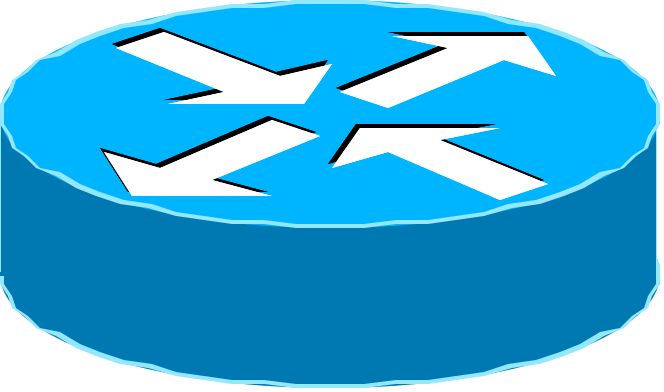
\includegraphics[width = 1cm]{switch.png}};
 \node[below] at (c1.south) {\huge $c_1$};
    \node (c2) at (8,2) {
\includegraphics[width = 1cm]{bbu.png}};
  \node[below] at (c2.south) {\huge $c_2$};
  


\path (s2) edge [->] node[anchor=south,inner sep = 0.2cm]{$3$} (c1);
\path (c1) edge [->] node[anchor=south,inner sep = 0.2cm]{$7$} (c2);
\path (c2) edge [->] node[anchor=south,inner sep = 0.2cm]{$4$} (t2);






\end{tikzpicture}
}

\caption{A route with two contention points and the weights of each arc. Vertex $c_2$ represents the BBU where messages may be buffered.}
\label{fig:routeexample}
\end{figure} 
 

    The {\bf weight of a vertex} $u_i$ in a route $r=(u_0,\dots,u_l)$ is defined by $\lambda(r,u_i)= \sum\limits_{0 \leq j <i} \omega(r,u_j)$. It is the time needed by a message to go from the first vertex of the route to $u_i$. The \textbf{length} of the route $r$ is defined by $\lambda(r)= \lambda(r,u_l)$. 

  	On each route, we choose to buffer the message only in the BBU. Since the BBU does not correspond to a contention point, we identify the BBU with the next contention point in the route. The set of these contention points with possible buffering is denoted by ${\cal B}$. Hence, in this article, each route has exactly one vertex in $\cal{B}$. We can now define the \textbf{routed network} which models the telecommunication network topology in this article, see Figure~\ref{fig:graphmodel.pdf} for an example. 


  	\begin{definition}
    A \textbf{routed network} is a triple $(\cal{R},\,\cal{B},\,\omega)$ where $\cal{R}$ is a set of routes, $\cal{B}$ a set of vertices and $\omega$ a weight function on the routes of $\cal{R}$. 
    \end{definition}
     


\begin{figure}
\centering

	
	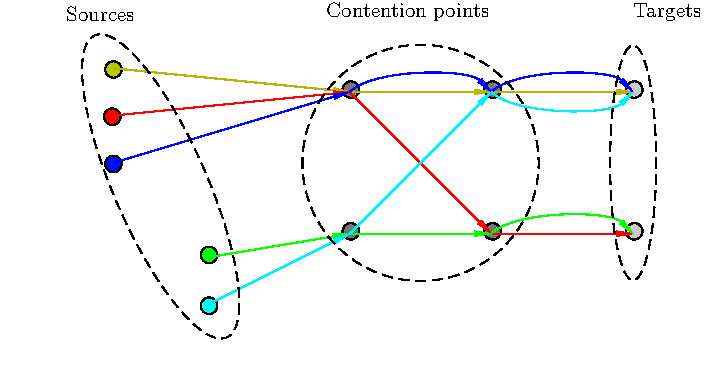
\includegraphics[scale=0.7]{graphmodel.pdf}\\

\caption{A routed network, each route is represented by a colored path. The BBUs are located in $c_2$ and $c_4$. Weights on the arcs are ommited.}
\label{fig:graphmodel}
\end{figure} 
 

	 
	 
 	\subsection{Dynamic of Datagrams Transmissions}
	    
 		In this article, we consider a discretized time. The unit of time is called a {\bf tic}. This is the time needed to send an atomic data in a link of the network. We assume that the speed of the links is the same over all the network. We are developing a prototype of this work based on Ethernet base-X~\cite{ieee_8023}, using standard values for the parameters of the network: the size of an atomic data is $64$ Bytes, the speed of the links is $10$Gbps, hence the duration of a tic is about $5.1$ nanoseconds. 

        In the process we study, a message, called a {\bf datagram}, is sent on each route from each source node of a route. The \textbf{size} of a datagram is an integer, denoted by $\tau$, it is the number of tics needed by a node to emit the full datagram in a link. In this paper, we assume that $\tau$ is the same for all routes. It is justified by our application to C-RAN, where all source nodes are RRHs sending the same type of datagram. There is no fragmentation: Once a datagram has been emitted, it cannot be fragmented during its travel in the network. 

        In order to avoid contention, it is possible to choose the emission time of the datagrams and also to buffer datagrams in contention points in $\cal{B}$.
        These choices are represented by an \textbf{assignment}, defined as follows.

         \begin{definition}
         An assignment $A$ of a routed network $(\cal{R},\,\cal{B},\,\omega)$ is a function which associates to each route $r \in \cal{R}$, the pair of integers $A(r) = (o_r,w_r)$.
         \end{definition}
        The value $o_r$ is the \textbf{offset} of the route $r$ in the assignment $A$, the time at which the datagram is sent from the first vertex of $r$.
         The value $w_r$ is the \textbf{waiting time} of the route $r$ in the assignment $A$: the datagram is buffered for $w_r$ tics in $u_j \in {\cal B} \cap r$, the vertex representing the BBU.
 		The \textbf{arrival time} of a datagram in the vertex $u_i$ of $r$, is the first time at which the datagram sent on $r$ reaches $u_i$, and is defined by $t(r,u_i) = \lambda(r,u_i) + o_r $ if 
 		$i \leq j$ and $t(r,u_i) = \lambda(r,u_i) + o_r + w_r$ otherwise.

        \begin{examplee}
        Consider the route $r$ of Figure~\ref{fig:routeexample} and an assignment such that $o_r=2$ and $w_r = 6$. The arrival times of a datagram are the following: $t(r,c_1) =  \lambda(r,c_1) + o_r =  3 + 2 = 5$, $t(r,c_2) = \lambda(r,c_2) + o_r = 12$ and  $t(r,t) = \lambda(r,t) + o_r + w_r  = 22$.
        \end{examplee}

 		 Let $u_l$ be the last vertex of the route $r$, the \textbf{transmission time} of the datagram on 
  		$r$ is denoted by $TR(r,A)$ and is equal to $\lambda(r) + w_r$ (also $t(r,u_l) - o_r$). This is the total time taken by the process we study: the sending of the datagram from the RRH to the BBU and the return of the answer back to the RRH. We can decompose this time into $\lambda(r)$, the \emph{physical latency} of the process and $w_r$, the \emph{logical latency}. 
  		We define the \textbf{transmission time} of an assignment $A$ as the worst transmission time of a route: $TR(A) = \displaystyle \max\limits_{r \in {\cal R}} TR(r,A)$. 
        Figure~\ref{fig:datagramtimeline} represents the different events happening during the lifetime  of a datagram  sent on a route $r$.
  		\begin{figure}
  		 \begin{center}
      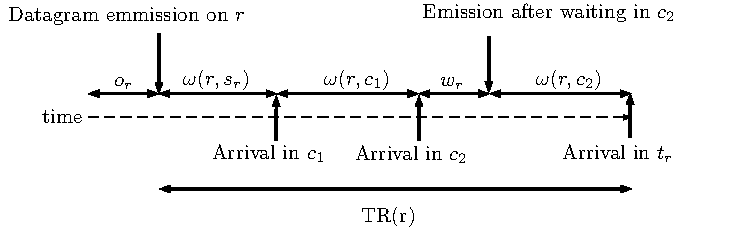
\includegraphics[width=\textwidth]{time.pdf}
      \end{center}
      \caption{Timeline of a datagram during its travel on a route $r = (s_r,c_1,c_2,t_r)$, with $c_2 \in \cal{B}$ and $A(r) = (o_r,w_r)$}
      \label{fig:datagramtimeline}
  		\end{figure}




 	\subsection{Periodic Emission of Datagrams}

	In the previous section, we have explained how \emph{one} datagram follows its route.
	However, the sources of datagrams we model in this article are \emph{periodic}: for each period of $P$ tics, a datagram is sent, from each source node in the network, at its offset. The process is assumed to be infinite, since it must work for an arbitrary number of periods. In this article, for a given route, we use the same offset and waiting time in all periods. This choice makes our problem more tractable from a theoretical perspective and allow for a much simpler implementation in real networks. As a consequence, at the same time of two different periods, all datagrams are at the same position in the network: the assignments built are themselves periodic of period $P$. Thus, we only need to consider the behavior of the datagrams on each node of the network during a single period, and to apply the same pattern to every subsequent period. 
 	Using a different offset for each route corresponds to sending their datagram at a different time in the period. This matches our hypothesis that the emissions of the RRHs need not being synchronized, but they share a common global clock, useful for coordination of their emissions.

 	Let $A$ be an assignment of a routed network $(\cal{R},\,\cal{B},\,\omega)$.
    Let us denote by $[r,u]_{P,\tau}$, the set of tics used by a datagram on the route $r$ at vertex $u$ in a period $P$, that is $[r,u]_{P,\tau} = \{t(r,u) + i \mod P \mid 0 \leq i < \tau \}$. This set of tics depends on $A$, but $A$ is omitted in the notation, since it is always clear from the context. We can now define the constraints that an assignment must respect to represent a \textbf{valid}
    sending process, for a given period $P$ and size $\tau$.


    \begin{definition}
    Let $r_1$ and $r_2$ be two routes of a routed network $N$, $A$ an assignment of $N$. The routes $r_1$ and $r_2$ have a collision at the contention point $u$ for the assignment $A$, if and only if $[r_1,u]_{P,\tau} \cap [r_2,u]_{P,\tau} \neq \emptyset$.
    \end{definition}
    
\begin{examplee}
Consider $P=6$, $\tau = 3$, and two routes $r_1$ and $r_2$ with a common contention point $c$. Take $o_1 = o_2 = 0$, $\lambda(r_1,c) = 5$ and $\lambda(r_2,c) = 1$ (this example is ilustrated by Figure~\ref{fig:cols}). Let the tics of a period be numbered from $0$ to $P-1$. Thus, we can compute $[r_1,c]_{P,\tau} =\{5,0,1\}$ and $[r_2,c]_{P,\tau} = \{1,2,3\}$. There is a collision because $[r_1,c]_{P,\tau}\cap[r_2,c]_{P,\tau}=\{1\} $. This collision can be avoided by taking $o_2=1$ in order to obtain $[r_2,c]_{P,\tau} = \{2,3,4\} $.
\end{examplee}
\begin{figure}
 
 \begin{center}
\scalebox{0.6}{

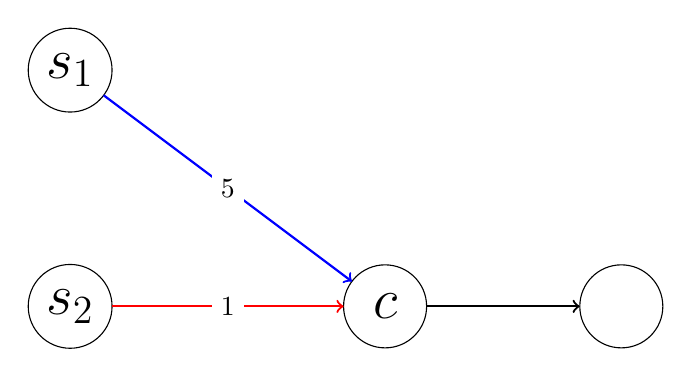
\begin{tikzpicture}
  \SetGraphUnit{5}
    \tikzset{
  EdgeStyle/.append style = {->} }
   \tikzstyle{VertexStyle}=[shape = circle, draw, minimum size = 30pt]
   \renewcommand{\VertexLightFillColor}{orange}
  \Vertex[x=0,y=3, L = {\huge $s_2$}]{a3};

  \Vertex[x=0,y=6, L = {\huge $s_1$}]{a1}


  \Vertex[x=4,y=3, L = {\huge $c$}]{c}

 \SetVertexNoLabel
\Vertex[x=7,y=3]{d}

      \Edge(c)(d)
  \tikzset{
  EdgeStyle/.append style = {blue} }
  \Edge[label = 5](a1)(c)   
 
  
    \tikzset{
  EdgeStyle/.append style = {red} }
    \Edge[label = 1](a3)(c)
  


\end{tikzpicture}


}\\

\vspace{0.5cm}
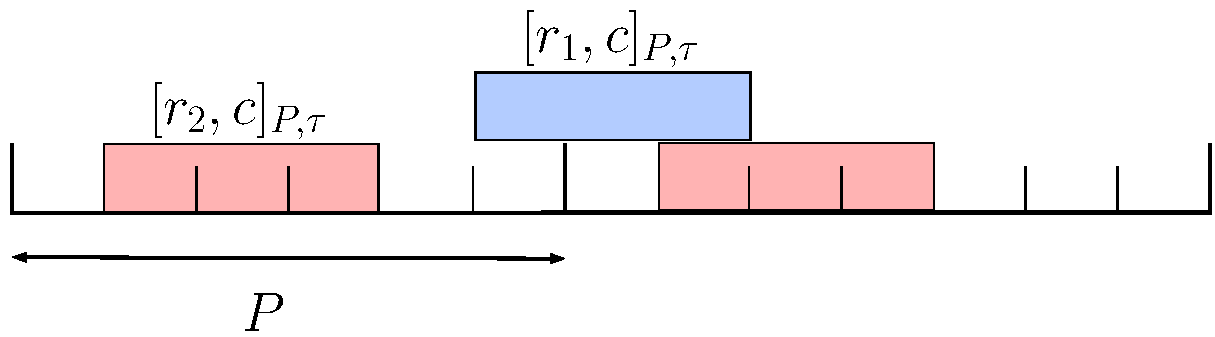
\includegraphics[width=0.6\textwidth]{cols}
\caption{A collision between two message due to the periodicity when $P=6$,$\tau=3$ and $o_1 = o_2 = 0$.}
\label{fig:cols}
\end{center}

\end{figure}

    \begin{definition}
    An assignment $A$ is valid if, for all contention points $u$ and routes $r_1$ and $r_2$ containing $u$, $r_1$ and $r_2$ have no collision at $u$ for $A$. 
    \end{definition}

    The validity of an assignment depends on $P$ the period and $\tau$ the size of the datagrams, thus if we need to mention these parameters, we say that $A$ is a \textbf{valid $(P,\tau)$-assignment}. When $P$ and $\tau$ are clear from the context, we denote $[r,u]_{P,\tau}$ by $[r,u]$ and say that $A$ is a valid assignment. 

\begin{examplee}

    Figure~\ref{fig:example} illustrates two valid assignments for different values of $P$ and $\tau$, but the same network. The three routes are depicted by three different colors. If we let $P = 2$ and $\tau = 1$, then there is a $(2,1)$-periodic valid assignment with waiting times zero by taking $0$ as offset for each route. However, for the same routed network but $P=5$ and $\tau = 2$, there is no solution to the problem with all waiting times zero. If we allow $1$ tic of waiting time for one route, we can build the valid assignment $A'(r_1) = (0,0)$, $A'(r_2) = (2,1)$, $A'(r_3)= (0,0)$.

\end{examplee}
  
\begin{figure}[ht]
    \begin{center}
        \scalebox{0.7}{
		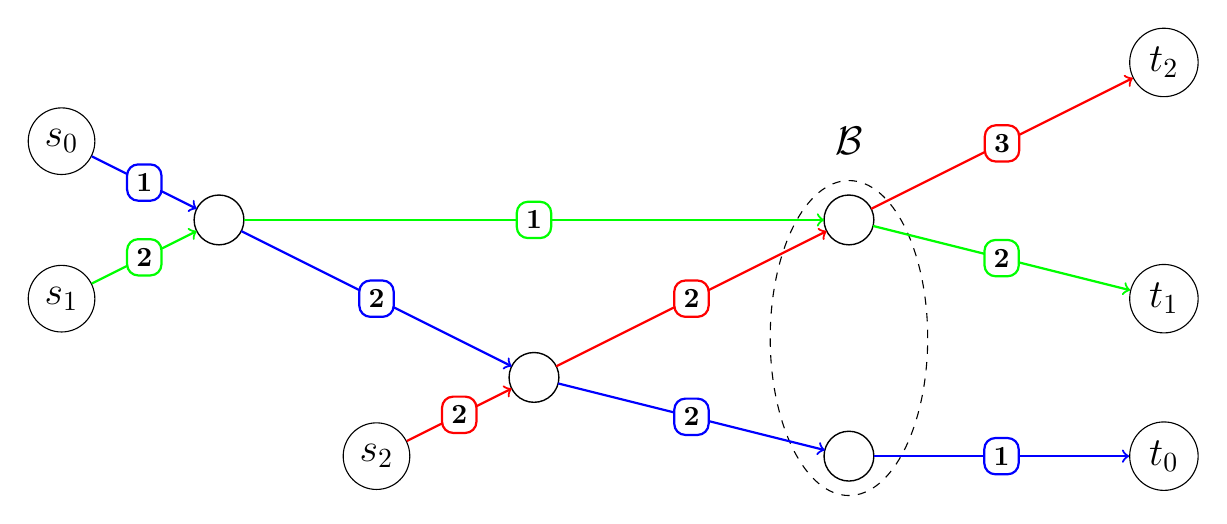
\begin{tikzpicture}
\tikzset{
  LabelStyle/.style = { rectangle, rounded corners, draw,
                       font = \bfseries },
  EdgeStyle/.append style = {->} }
  \SetGraphUnit{5}
  \node[draw,circle] (s3) at (4, 2) {\Large $s_2$}; 
  \node[draw,circle] (s2) at (0, 4) {\Large $s_1$}; 
  \node[draw,circle] (s1) at (0, 6) {\Large $s_0$}; 

  \node[draw,circle] (t3) at (14, 7) {\Large $t_2$}; 
  \node[draw,circle] (t2) at (14, 4) {\Large $t_1$}; 
  \node[draw,circle] (t1) at (14, 2) {\Large $t_0$}; 

   \node[circle] (buf) at (10, 6) {\Large $\cal{B}$};
  \SetVertexNoLabel
  \Vertex[x=2,y=5]{A}
    \Vertex[x=10,y=2]{B}
  \Vertex[x=10,y=5]{C}

  \Vertex[x=6,y=3]{E}
     \draw[dashed] (10,3.5) ellipse  (1cm and 2cm);
  \tikzset{
  EdgeStyle/.append style = {green} }
  \Edge[label = 2](s2)(A)

  \Edge[label = 1](A)(C)
 
  \Edge[label = 2](C)(t2)

  
   \tikzset{
  EdgeStyle/.append style = {red} }
  \Edge[label = 2](s3)(E)
  \Edge[label = 2](E)(C)
  \Edge[label = 3](C)(t3) 

     \tikzset{
  EdgeStyle/.append style = {blue} }
  \Edge[label = 1](s1)(A)
  \Edge[label = 2](A)(E)
  \Edge[label = 2](E)(B)
 \Edge[label = 1](B)(t1)

\end{tikzpicture}

}
  	\end{center}
    \caption{A routed network with $A(\textcolor{blue}{r_1})= \textcolor{blue}{(0,0)}$,
    $A(\textcolor{green}{r_2}) = \textcolor{green}{(0,0)}$, $A(\textcolor{red}{r_3}) = \textcolor{red}{(0,0)}$ as a $(2,1)$-periodic valid assignment and $A'(\textcolor{blue}{r_1})= \textcolor{blue}{(0,0)}$,
    $A'(\textcolor{green}{r_2}) = \textcolor{green}{(2,1)}$, $A'(\textcolor{red}{r_3}) = \textcolor{red}{(0,0)}$ as a $(5,2)$-periodic valid assignment}
    \label{fig:example}
\end{figure}



	\subsection{Valid Assignment with Low Latency}

      The period $P$, as well as the size of a datagram $\tau$ are fixed in our C-RAN settings, but not the buffering policy. Hence, the aim of this article is to find a valid assignment which minimizes the worst latency of the transmissions over the network, that is $TR(A)$. We formally introduce the problem we want to solve in this article. 

      \bigskip

      \noindent \textbf{ Minimal Transmission Time }(\mintra)

      \noindent {\bf Input:} A routed network $N$, integers $P$ and $\tau$.
      
      \noindent {\bf Question:} Find the minimum value $TR(A)$ for all $A$ valid $(P,\tau)$ assignments of $N$. 
      \bigskip

      For simpler hardness proofs and easier reductions, we rather study the decision version of \mintra, that we call \pall for \textbf{P}eriodic \textbf{A}ssignment for \textbf{L}ow \textbf{L}atency. Each route must respect a time limit called a \emph{deadline}. These limits are encoded in a deadline function $d$, which maps to each route $r$ an integer such that $TR(r,A)$ must be less than $d(r)$.
      

      \bigskip

      \noindent {\bf Periodic Assignment with Low Latency} (\pall)

      \noindent {\bf Input:}  A routed network $N$, integers $P$ and $\tau$ and a deadline function $d$.
      
      \noindent {\bf Question:} Does there exist a valid $(P,\tau)$ assignment $A$ of $N$ such that for all $r \in {\cal R}$, $TR(r,A) \leq d(r)$?
      \bigskip

	  In the next subsection, this problem is proved to be $\NP$-hard. In Section~\ref{sec:PALL}, we propose heuristics solving the search version of \pall (computing a valid assignment), also denoted by \pall for simplicity. In the definition of \pall, we have chosen to bound the transmission time of each route, in particular we control the worst case latency. It is justified by our C-RAN application with hard constraints on the latency. 

	 We say that an assignment is \textbf{bufferless} when the waiting time of all routes are zero.
	 The assignment can then be seen as a function from the routes to the integers (the value of the offset, the waiting time is omitted). We consider a restricted version of \pall, requiring to find a bufferless assignment. This is equivalent to using the deadline function $d(r) = \lambda(r)$ (the transmission time must be equal to the size of the route), which implies $w_r = 0$ for all $r \in \cal{R}$. This problem is called \textbf{P}eriodic \textbf{A}ssignment for \textbf{Z}ero \textbf{L}atency and is denoted by \pazl. 

     \bigskip

      \noindent {\bf Periodic Assignment with Zero Latency }(\pazl)

      \noindent {\bf Input:}  A routed network $N$, integers $P$ and $\tau$.
      
      \noindent {\bf Question:} Does there exist a valid bufferless $(P,\tau)$ assignment of $N$?
      \bigskip


     Studying \pazl is simpler: in an instance, there is no need to precise $\cal{B}$ in the routed network nor the deadline function and a solution is just an offset for each route.  Moreover, a solution to \pazl is more efficient when implemented in real telecommunication networks, since we do not need contention buffer at all. A switch taking full advantage of the absence of buffer is presented in~\cite{Marc2201:Experimental}. 
      An unusual property of assignments is that given a routed network and a deadline, we may have a $(P,\tau)$ assignment but no $(P',\tau)$ assignment with $P' > P$: the existence of an assignment is not monotone with regard to $P$.

	\begin{proposition} \label{prop:monotonic}
	 For any odd $P$, there is a routed network with a $(2,1)$-periodic bufferless assignment but no $(P,1)$-periodic bufferless assignment.
	\end{proposition}

	\begin{proof}
      Let us build $N$, a generalization of the routed network given in Figure~\ref{fig:example}. 
      Let $n$ be an integer, the vertices of the routes are $v_{i,j}$, $v_i^1$ and $v_i^2$, with $0 \leq i < j <n$. 
      There are $n$ routes denoted by $r_i$, for $i \in [n]$. The route $r_i$ is equal to $(v_i^1,v_{i,1},\dots,v_{i,n-1},v_i^2)$. The weights of the arcs are set so that $\lambda(r_i, v_{i,j}) - \lambda(r_j,v_{i,j})= P$, where $P$ is an odd number smaller than $n$. It is always possible by choosing appropriate values for $\omega(r_i,v_{i,j-1})$ and $\omega(r_j,v_{i-1,j})$. In such a graph, there is no bufferless $(P,\tau)$ assignment, since the problem reduces to finding a $P$-coloring in a complete graph with $n > P$ vertices, the colors being the offsets of the routes.


      If we consider a period of $2$, for all $i \neq j$, $\lambda(r_i, v_{i,j}) - \lambda(r_j, v_{i,j}) \mod 2 = 1$, hence two datagrams of same offset and size $1$ do not have a collision at $v_{i,j}$. Therefore, the bufferless assignment defined by $A(r_i) = 0$ for all $i \in [n]$ is a valid $(2,1)$ assignment of $N$.      
\end{proof}



      The table of Figure~\ref{tab:summary} summarizes the main notations used in the paper.
    \begin{figure}
      \begin{center}
    \begin{tabularx}{\textwidth}{|c|X|}
    \hline
     $N = (\cal{R},\,\cal{B},\,\omega)$ & Routed network \\
     \hline
     $n = |\cal{R}|$ & Number of routes\\
     \hline
     $P$ & Period\\
     \hline
     $\tau$ & Size of a datagram\\
     \hline
     $\omega(r,u)$ & Weight of the arc $(u,v)$ of $r$ \\
     \hline
     $\lambda(r,u)$ & Length of the route $r$ up to vertex $u$\\
     \hline
     $\lambda(r)$ & Length of the route $r$\\
     \hline 
     $A$ & Assignment\\
     \hline 
     $A(r) = (o_r,w_r)$ & Offset and waiting time of the route $r$ given by $A$ \\
     \hline 
     $TR(A,r)$& Transmission time of the route $r$ for the assignment $A$\\
     \hline 
     $TR(A)$& Transmission time of the assignment $A$\\
     \hline
     $d(r)$ & Deadline of the route $r$\\
     \hline
	 $t(r,u)$ & Transmission time on the route $r$, up to the vertex $u$\\
     \hline
     $ [r,u]$ & Tics used in the period by the route $r$ at vertex $u$\\
     \hline
      \end{tabularx}
      \end{center}
      \caption{Summary of the notations of the article.}\label{tab:summary}
    \end{figure}
  	
  	Let us introduce a few parameters quantifying the complexity of a routed network.
	The \textbf{contention depth} of a routed network is the size of the longest route (number of arcs) of the network minus one. It is the number of contention points on the route, since the first and the last vertex are private to the route. The \textbf{width} of a vertex is the number of routes which contains it, equivalently its indegree or its outdegree. By definition, 
	the first and last vertex of a route are of width one, while all other vertices are of width at least two (otherwise they are removed).
	The \textbf{contention width} of a routed network is the maximal width of its vertices. 
	A valid $(P,\tau)$ assignment of a routed network must satisfy that $P/\tau$ is larger or equal to the contention width. Now, let us fix $P$ and $\tau$, for a given vertex of contention width $c$, we define its \textbf{load} as $c\tau/P$. It represents the proportion of the period used by datagrams at this contention point. The load of the routed network is the maximum of the loads of its vertices. A routed network must have a load less or equal to one to admit a valid assignment.



    \subsection{The Star Routed Network} \label{sec:star_routed_network}
  
	In this section, we define a family of simple routed networks modeling a Multipoint-to-Multipoint fronthaul (see figure~\ref{fig:star}), which has been designed for C-RAN \cite{tayq2017real}. Let $N = (\cal{R},\,\cal{B},\,\omega)$ be a routed network, we say it is a \textbf{star routed network} if and only if ${\cal R} =\{r_0,\dots,r_{n-1}\}$ where for $0 \leq i<n$, $r_i = (s_i,c_1,c_2,t_i)$ and ${\cal B} = \{ c_2 \}$ (datagrams can wait in $c_2$). Star routed networks have contention depth two but a maximal contention width of $n$. The load on each of the two contention points is thus $n\tau / P$.

	The fronthaul network we model with star routed network has a single shared link, which connects all RRHs at one end and all BBUs at the other end. The links are all \emph{full-duplex}, meaning that the datagrams going from RRHs to BBUs do not interact with those going in the other direction. 
	 This property does not need to be enforced in our theoretical modeling, but it matches real fronthaul network, and we will use such examples for our experiments. 
	 
	The two contention points $c_1$ and $c_2$ model the beginning of the shared link (used to go from the RRHs to the BBUs) and the other end of the shared link (used in the other direction). 
	The computation in the BBU of an answer to a datagram on the route $r$ takes some time.
	In the star routed network, this time is encoded in the weight of the arc between $c_1$ and $c_2$ in $r$. The weight $\omega(r,c_1)$ is the time needed to go through the shared link, then to arrive at the BBU, plus the computation time and the time to return to the shared link, see Figure~\ref{fig:star}.

	Star routed networks are simple, but every network in which all routes share an arc and satisfy a coherent routing condition can be modeled by a star routed network.
	Fronthaul networks where all the BBUs are located in the same data center are star routed networks. In such a situation, we can consider the weights of the arcs $(c_1,c_2)$ to be either all equals (in that case \pazl is trivial, see Section~\ref{sec:PALL}) or different due to the structure of the network inside the data center and the various hardwares used for the BBUs, computing with different speeds. 

      
     
  % \begin{minipage}{0.40\linewidth}
    %	\includegraphics[scale=0.5]{starfronthaul}\\
    	


 %  \end{minipage}\hfill
%\begin{minipage}{0.55\linewidth}   

\begin{figure}
\begin{center}
\scalebox{0.4}{

\begin{tikzpicture}
  \SetGraphUnit{5}
    \tikzset{
  EdgeStyle/.append style = {->} }
   \tikzstyle{VertexStyle}=[shape = circle, draw, minimum size = 30pt]
 

  \node (s1) at (0,4) {
\includegraphics[width = 1cm]{rrh.png}};
  \node[below] at (s1.south) {\huge $r_1$};
  \node (s2) at (0,2) {
\includegraphics[width = 1cm]{rrh.png}};
  \node[below] at (s2.south) {\huge $r_2$};
  \node (s3) at (0,0) {
\includegraphics[width = 1cm]{rrh.png}};
  \node[below] at (s3.south) {\huge $r_3$};
  
   \node (t1) at (12,4) {
\includegraphics[width = 1cm]{bbu.png}};
  \node[below] at (t1.south) {\huge $b_1$};
  \node at (t1.north west) {\textcolor{red}{3}};
  \node (t2) at (12,2) {
\includegraphics[width = 1cm]{bbu.png}};
  \node[below] at (t2.south) {\huge $b_2$};
   \node at (t2.north west) {\textcolor{red}{2}};
  \node (t3) at (12,0) {
\includegraphics[width = 1cm]{bbu.png}};
  \node[below] at (t3.south) {\huge $b_3$};
   \node at (t3.north west) {\textcolor{red}{3}};
    \node (c1) at (4,2) {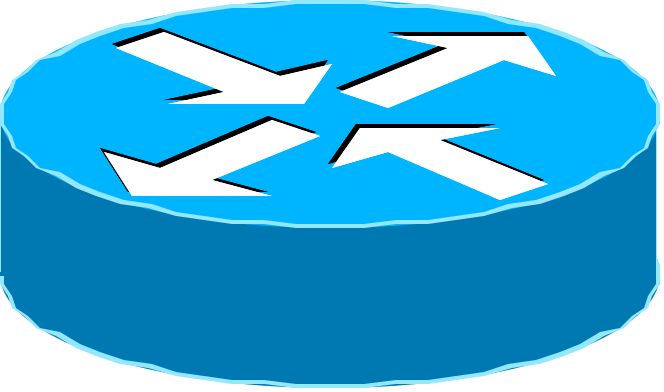
\includegraphics[width = 1cm]{switch.png}};
  
    \node (c2) at (8,2) {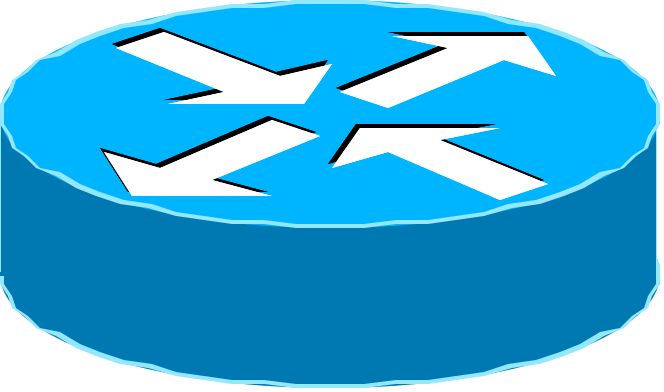
\includegraphics[width = 1cm]{switch.png}};
  
  
 %\SetVertexNoLabel
  %\Vertex[x=4,y=2]{n1}

  %\Edge[label = $5$](s1)(c1)
  %\Edge[label = $7 + 4+4$](c1)(c2)
  %\Edge[label = $3$](s2)(c1)
   %\Edge[label = $7$](s3)(c1)
  %  \Edge[label = $7+3$](c2)(s2p)
 %  \Edge[label = $7+7$](c2)(s3p)
%\Edge[label = $7 + 5$](c2)(s1p)
\path (s1) edge [<->] node[anchor=south,inner sep = 0.2cm]{$5$} (c1);

\path (s2) edge [<->] node[anchor=south,inner sep = 0.2cm]{$3$} (c1);
\path (s3) edge [<->] node[anchor=south,inner sep = 0.2cm]{$7$} (c1);
\path (c2) edge [<->] node[anchor=south,inner sep = 0.2cm]{$4$} (t2);
\path (c2) edge [<->] node[anchor=south,inner sep = 0.2cm]{$1$} (t3);

\path (c2) edge [<->] node[anchor=south,inner sep = 0.2cm]{$2$} (t1);

%\path (c2) edge [<-,double] node[anchor=south,inner sep = 0.2cm]{$7$} (c1);
%\path (c2) edge [->,bend left=1] node[anchor=south,inner sep = 0.2cm]{$7$} (c1);
%\node[below] at (5,1.8) {\huge $c_1$};
%\node[below] at (6,1.8) {7};
%\node[above] at (7,2.2) {\huge $c_2$};
\node[above] at (6,1.75) {7};
% \draw[->] (4.5,1.85) -- (7.5,1.85)   ;
% \draw[<-] (4.5,2.15) -- (7.5,2.15)   ;
 \path (c1) edge [<-,bend left=15] node[anchor=south,inner sep = 0.2cm]{\huge $c_2$} (c2);
\path (c1) edge [->,bend right=15] node[anchor=north,inner sep = 0.2cm]{\huge $c_1$} (c2);

  \Vertex[x=14,y=4, L = {\huge $s_1$}]{s1};
  \Vertex[x=14,y=2, L = {\huge $s_2$}]{s2};
\Vertex[x=14,y=0, L = {\huge $s_3$}]{s3};
\Vertex[x=26,y=4, L = {\huge $t_1$}]{s1p};
\Vertex[x=26,y=2, L = {\huge $t_2$}]{s2p};
\Vertex[x=26,y=0, L = {\huge $t_3$}]{s3p};
\Vertex[x=22,y=2, L = {\huge $c_2$}]{c2};

  \Vertex[x=18,y=2, L = {\huge $c_1$}]{c1}
  
 %\SetVertexNoLabel
  %\Vertex[x=4,y=2]{n1}

  %\Edge[label = $5$](s1)(c1)
  %\Edge[label = $7 + 4+4$](c1)(c2)
  %\Edge[label = $3$](s2)(c1)
   %\Edge[label = $7$](s3)(c1)
  %  \Edge[label = $7+3$](c2)(s2p)
 %  \Edge[label = $7+7$](c2)(s3p)
%\Edge[label = $7 + 5$](c2)(s1p)
\path (s1) edge [->] node[anchor=south,inner sep = 0.2cm]{$5$} (c1);

\path (s2) edge [->] node[anchor=south,inner sep = 0.2cm]{$3$} (c1);
\path (s3) edge [->] node[anchor=south,inner sep = 0.2cm]{$7$} (c1);
\path (c2) edge [->] node[anchor=south,inner sep = 0.2cm]{$7+3$} (s2p);
\path (c2) edge [->] node[anchor=south,inner sep = 0.2cm]{$7+7$} (s3p);

\path (c2) edge [->] node[anchor=south,inner sep = 0.2cm]{$7+5$} (s1p);

\path (c1) edge [->] node[anchor=south,inner sep = 0.2cm]{$7+4+\textcolor{red}{2}+4$} (c2);

\path (c1) edge [->,bend left=30] node[anchor=south,inner sep = 0.2cm]{$7+2+\textcolor{red}{3}+2$} (c2);
\path (c1) edge [->,bend right=30] node[anchor=north,inner sep = 0.2cm]{$7+1+\textcolor{red}{3}+1$} (c2);
   \node[circle] (buf) at (22, 0.5) {$\cal{B}$};
   \draw[dashed] (22,2) ellipse  (0.6cm and 1cm);
  %\draw[->,line width=0.5pt] (5,2.51) parabola bend (7.5,3.5) (10,2.51);
 %\draw[->,line width=0.5pt] (5,1.49) parabola bend (7.5,0.5) (10,1.49);
 

\end{tikzpicture}
}



%\end{minipage}

             \caption{Left, a physical fronthaul network and right, the star routed network modeling a round trip in the fronthaul network. The computation time in the BBU is given in red.}

	         \label{fig:star}
            \end{center}
	         \end{figure}
	         
  When solving \pall or \pazl on a star routed network, a period, a datagram size and a deadline function are also given. When the period is fixed, we modify the deadline function to do several simplifying assumptions on the parameters of the star routed network without loss of generality. We say that a star routed network is \textbf{canonical}, for a period $P$, if the weights of the arcs between $c_1$ and $c_2$ are in $[P]$ and the others are equal to zero. Hence, $\lambda(r_i)$, the length of a route is equal to the length of its arc $(c_1,c_2)$. Moreover, $\lambda(r_0) = 0$. See Figure~\ref{fig:canonical} for an example of the canonical star routed network of Figure~\ref{fig:star}.  
  
\begin{figure}
\begin{center}




 \scalebox{0.5}{

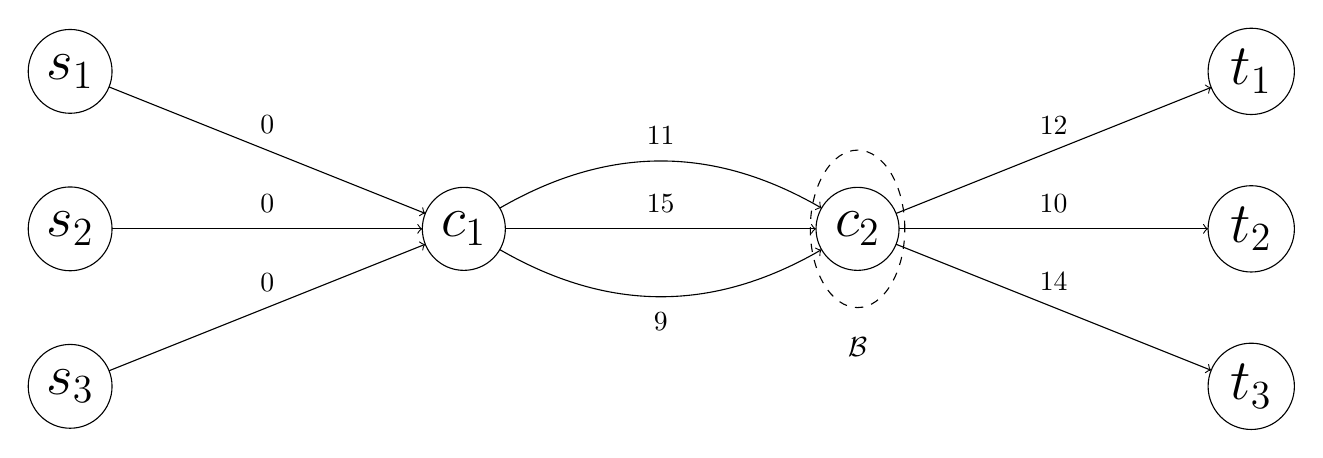
\begin{tikzpicture}
  \SetGraphUnit{5}
    \tikzset{
  EdgeStyle/.append style = {->} }
   \tikzstyle{VertexStyle}=[shape = circle, draw, minimum size = 30pt]
   \renewcommand{\VertexLightFillColor}{orange}
  \Vertex[x=0,y=4, L = {\huge $s_1$}]{s1};
  \Vertex[x=0,y=2, L = {\huge $s_2$}]{s2};
\Vertex[x=0,y=0, L = {\huge $s_3$}]{s3};
\Vertex[x=15,y=4, L = {\huge $t_1$}]{s1p};
\Vertex[x=15,y=2, L = {\huge $t_2$}]{s2p};
\Vertex[x=15,y=0, L = {\huge $t_3$}]{s3p};
\Vertex[x=10,y=2, L = {\huge $c_2$}]{c2};

  \Vertex[x=5,y=2, L = {\huge $c_1$}]{c1}
  
 %\SetVertexNoLabel
  %\Vertex[x=4,y=2]{n1}

  %\Edge[label = $5$](s1)(c1)
  %\Edge[label = $7 + 4+4$](c1)(c2)
  %\Edge[label = $3$](s2)(c1)
   %\Edge[label = $7$](s3)(c1)
  %  \Edge[label = $7+3$](c2)(s2p)
 %  \Edge[label = $7+7$](c2)(s3p)
%\Edge[label = $7 + 5$](c2)(s1p)
\path (s1) edge [->] node[anchor=south,inner sep = 0.2cm]{$0$} (c1);

\path (s2) edge [->] node[anchor=south,inner sep = 0.2cm]{$0$} (c1);
\path (s3) edge [->] node[anchor=south,inner sep = 0.2cm]{$0$} (c1);
\path (c2) edge [->] node[anchor=south,inner sep = 0.2cm]{$10$} (s2p);
\path (c2) edge [->] node[anchor=south,inner sep = 0.2cm]{$14$} (s3p);

\path (c2) edge [->] node[anchor=south,inner sep = 0.2cm]{$12$} (s1p);

\path (c1) edge [->] node[anchor=south,inner sep = 0.2cm]{$15$} (c2);

\path (c1) edge [->,bend left=30] node[anchor=south,inner sep = 0.2cm]{$11$} (c2);
\path (c1) edge [->,bend right=30] node[anchor=north,inner sep = 0.2cm]{$9$} (c2);
   \node[circle] (buf) at (10, 0.5) {$\cal{B}$};
   \draw[dashed] (10,2) ellipse  (0.6cm and 1cm);
  %\draw[->,line width=0.5pt] (5,2.51) parabola bend (7.5,3.5) (10,2.51);
 %\draw[->,line width=0.5pt] (5,1.49) parabola bend (7.5,0.5) (10,1.49);
 

\end{tikzpicture}
}

 $d_1 = 25$, $d_2 = 31$, $d_3 = 25$

$\downarrow$


 \scalebox{0.5}{

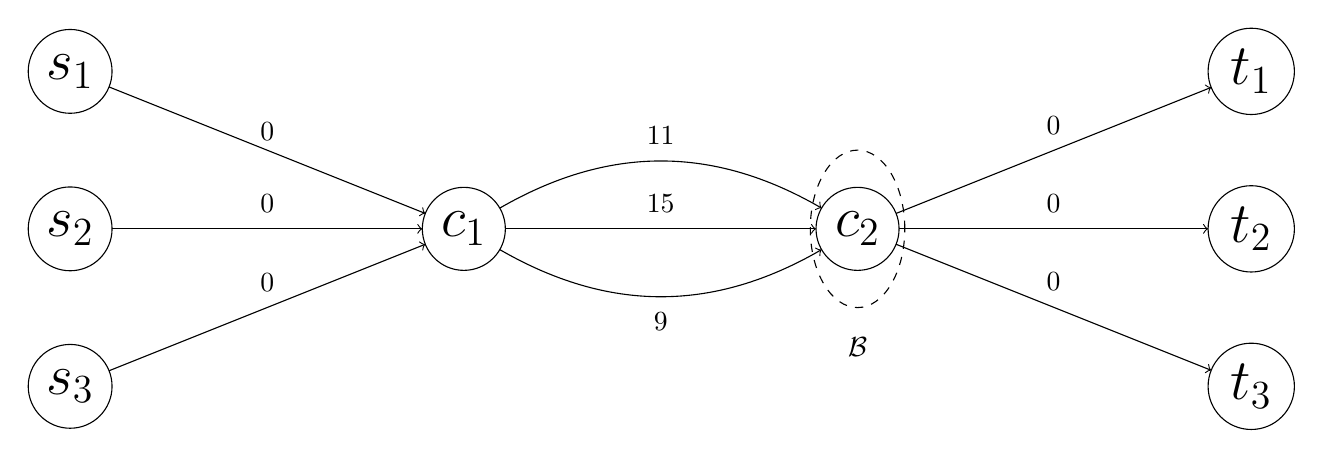
\begin{tikzpicture}
  \SetGraphUnit{5}
    \tikzset{
  EdgeStyle/.append style = {->} }
   \tikzstyle{VertexStyle}=[shape = circle, draw, minimum size = 30pt]
   \renewcommand{\VertexLightFillColor}{orange}
  \Vertex[x=0,y=4, L = {\huge $s_1$}]{s1};
  \Vertex[x=0,y=2, L = {\huge $s_2$}]{s2};
\Vertex[x=0,y=0, L = {\huge $s_3$}]{s3};
\Vertex[x=15,y=4, L = {\huge $t_1$}]{s1p};
\Vertex[x=15,y=2, L = {\huge $t_2$}]{s2p};
\Vertex[x=15,y=0, L = {\huge $t_3$}]{s3p};
\Vertex[x=10,y=2, L = {\huge $c_2$}]{c2};

  \Vertex[x=5,y=2, L = {\huge $c_1$}]{c1}
  
 %\SetVertexNoLabel
  %\Vertex[x=4,y=2]{n1}

  %\Edge[label = $5$](s1)(c1)
  %\Edge[label = $7 + 4+4$](c1)(c2)
  %\Edge[label = $3$](s2)(c1)
   %\Edge[label = $7$](s3)(c1)
  %  \Edge[label = $7+3$](c2)(s2p)
 %  \Edge[label = $7+7$](c2)(s3p)
%\Edge[label = $7 + 5$](c2)(s1p)
\path (s1) edge [->] node[anchor=south]{$0$} (c1);

\path (s2) edge [->] node[anchor=south,inner sep = 0.2cm]{$0$} (c1);
\path (s3) edge [->] node[anchor=south,inner sep = 0.2cm]{$0$} (c1);
\path (c2) edge [->] node[anchor=south,inner sep = 0.2cm]{$0$} (s2p);
\path (c2) edge [->] node[anchor=south,inner sep = 0.2cm]{$0$} (s3p);

\path (c2) edge [->] node[anchor=south,inner sep = 0.2cm]{$0$} (s1p);

\path (c1) edge [->] node[anchor=south,inner sep = 0.2cm]{$15$} (c2);

\path (c1) edge [->,bend left=30] node[anchor=south,inner sep = 0.2cm]{$11$} (c2);
\path (c1) edge [->,bend right=30] node[anchor=north,inner sep = 0.2cm]{$9$} (c2);
   \node[circle] (buf) at (10, 0.5) {$\cal{B}$};
   \draw[dashed] (10,2) ellipse  (0.6cm and 1cm);
  %\draw[->,line width=0.5pt] (5,2.51) parabola bend (7.5,3.5) (10,2.51);
 %\draw[->,line width=0.5pt] (5,1.49) parabola bend (7.5,0.5) (10,1.49);
 

\end{tikzpicture}
}

 $d_1 = 14$, $d_2 = 21$, $d_3 = 11$

$\downarrow$


 \scalebox{0.5}{

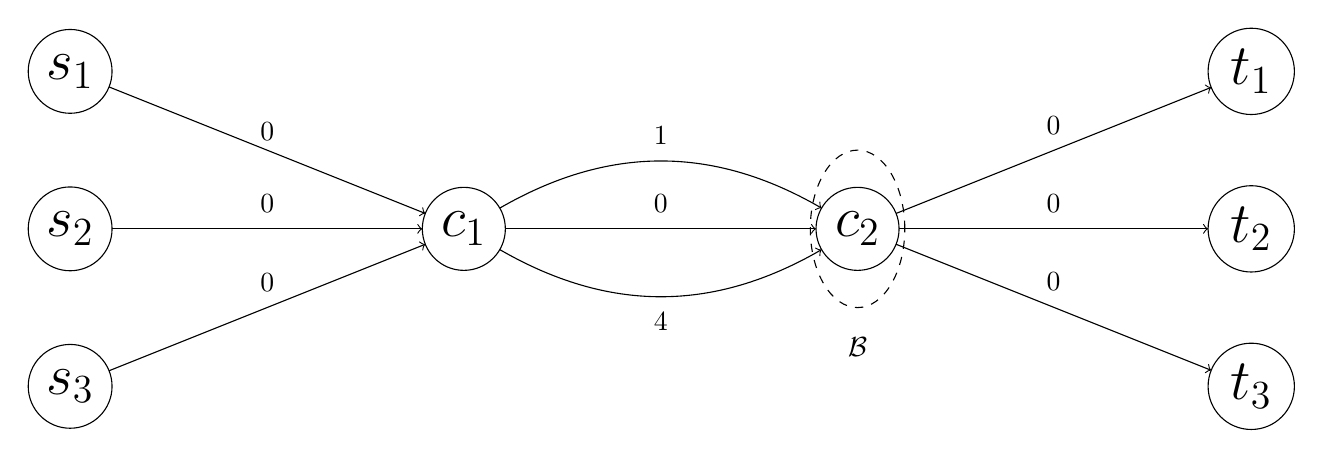
\begin{tikzpicture}
  \SetGraphUnit{5}
    \tikzset{
  EdgeStyle/.append style = {->} }
   \tikzstyle{VertexStyle}=[shape = circle, draw, minimum size = 30pt]
   \renewcommand{\VertexLightFillColor}{orange}
  \Vertex[x=0,y=4, L = {\huge $s_1$}]{s1};
  \Vertex[x=0,y=2, L = {\huge $s_2$}]{s2};
\Vertex[x=0,y=0, L = {\huge $s_3$}]{s3};
\Vertex[x=15,y=4, L = {\huge $t_1$}]{s1p};
\Vertex[x=15,y=2, L = {\huge $t_2$}]{s2p};
\Vertex[x=15,y=0, L = {\huge $t_3$}]{s3p};
\Vertex[x=10,y=2, L = {\huge $c_2$}]{c2};

  \Vertex[x=5,y=2, L = {\huge $c_1$}]{c1}
  
 %\SetVertexNoLabel
  %\Vertex[x=4,y=2]{n1}

  %\Edge[label = $5$](s1)(c1)
  %\Edge[label = $7 + 4+4$](c1)(c2)
  %\Edge[label = $3$](s2)(c1)
   %\Edge[label = $7$](s3)(c1)
  %  \Edge[label = $7+3$](c2)(s2p)
 %  \Edge[label = $7+7$](c2)(s3p)
%\Edge[label = $7 + 5$](c2)(s1p)
\path (s1) edge [->] node[anchor=south]{$0$} (c1);

\path (s2) edge [->] node[anchor=south,inner sep = 0.2cm]{$0$} (c1);
\path (s3) edge [->] node[anchor=south,inner sep = 0.2cm]{$0$} (c1);
\path (c2) edge [->] node[anchor=south,inner sep = 0.2cm]{$0$} (s2p);
\path (c2) edge [->] node[anchor=south,inner sep = 0.2cm]{$0$} (s3p);

\path (c2) edge [->] node[anchor=south,inner sep = 0.2cm]{$0$} (s1p);

\path (c1) edge [->] node[anchor=south,inner sep = 0.2cm]{$0$} (c2);

\path (c1) edge [->,bend left=30] node[anchor=south,inner sep = 0.2cm]{$1$} (c2);
\path (c1) edge [->,bend right=30] node[anchor=north,inner sep = 0.2cm]{$4$} (c2);
   \node[circle] (buf) at (10, 0.5) {$\cal{B}$};
   \draw[dashed] (10,2) ellipse  (0.6cm and 1cm);
  %\draw[->,line width=0.5pt] (5,2.51) parabola bend (7.5,3.5) (10,2.51);
 %\draw[->,line width=0.5pt] (5,1.49) parabola bend (7.5,0.5) (10,1.49);
 

\end{tikzpicture}
}

 $d_1 = 4$, $d_2 = 6$, $d_3 = 6$
 
\end{center}

\caption{Transformation of the star routed network of Figure~\ref{fig:star} into its canonical form, using the method of Proposition~\ref{prop:canonical}. Initially $\tau = 1$, $P=5$, $d_1 = 30$, $d_2 = 34$, $d_3 = 32$.}
\label{fig:canonical}
\end{figure}

  \begin{proposition}\label{prop:canonical}
   Let $I = (N, P, \tau , d)$, with $N = (\cal{R},\,\cal{B},\,\omega)$ a star routed network, then there is 
   $I' = (N', P, \tau , d')$, with  $N' = (\cal{R},\,\cal{B},\,\omega')$ a canonical star routed network, such that:
     $$I \in \pall \Leftrightarrow I' \in \pall \text{ and } I \in \pazl \Leftrightarrow I' \in \pazl$$
  \end{proposition}

  \begin{proof}
  We define $\omega'$ and $d'$ from $\omega$ and $d$ in such a way that there is a bijection 
  between valid assignments of $I$ and $I'$, which proves the proposition. In this bijection,
  the offsets $o_i$ for an assignment of $I$ will be mapped to $o'_i$, while the waiting times remain the same.
  
  The routed network $N'$ is equal to $N$ except for the weight function $\omega'$.
  We set the weights of the arcs $(s_i,c_1)$ to zero in $N'$. We obtain the bijection between valid assignments of $I$ and $I'$ by setting $o_i' + \omega(r_i,s_i) = o_i $ and $d'(r_i) = d(i) - \omega(r_i,s_i)$. The weights $\omega'(r_i,c_2)$ are also set to $0$, it does not change the possible collisions
  for an assignment but it changes the transmission time, hence we set $d'(r_i) = d'(r_i) - \omega(r_i,c_2)$
  to preserve the bijection between valid assignments of $I$ and $I'$. 

  We let $\omega'(r_i,c_1) = \omega(r_i,c_1) \mod P$. Again, it does not change collisions, since computing a possible collision is done modulo $P$. However, we must change $d'$ to be $d'(r_i) = d'(r_i) - \omega(r_i,c_1) + \omega'(r_i,c_1)$ to keep the same constraints on the transmission times of valid assignments.

  Finally, we assume w.l.o.g. that $\omega'(r_0,c_1)$ is the smallest weight among the weights of the arcs
  $(c_1,c_2)$. We let $\omega'(r_i,c_1) = \omega'(r_i,c_1) - \omega'(r_0,c_1)$, which implies that $\omega'(r_0,c_1) = 0$.  All weights of arcs $(c_1,c_2)$ are changed by the same value, hence collisions are not modified. We change $d'(r_i)$ to  $d'(r_i) - \omega'(r_0,c_1)$ for all $i$ so that the constraints on the deadlines stay the same.
  \end{proof}

   From now on, we may assume that a star routed network is canonical, using Proposition~\ref{prop:canonical}. To give an instance of \pall where the routed network is a canonical star routed network, it is enough to give the weights of the arcs $(c_1,c_2)$ for all routes, the period, the datagram size, and $d$ the deadline function. For an instance of \pazl we can also omit $d$.


\section{Hardness of \texttt{PALL} and \texttt{PAZL}}
  \label{sec:complexity}


	We show in this section that \pall is $\NP$-hard by proving $\NP$-hardness for a restricted version: \pazl with $\tau = 1$. We give two proofs that \pazl is $\NP$-complete.
	The first proof works even for contention depth two, but not for star routed networks.
	 For contention depth one, the problem is trivial: either the load is less than one and there is a valid bufferless assignment, or there is no valid assignment. 
	 The second proof works for graphs with contention width $2$: the conflicts are locally very simple, but the problem is complex globally nonetheless. Solving \pall is trivial on trees because they can be reduced to one vertex of contention depth one. Thus, it may be interesting to study its complexity on bounded treewidth (or dagwidth) networks, a common property of real networks~\cite{de2011treewidth}
 

 \begin{theorem}
\pazl is $\NP$-complete on the class of routed networks with contention depth 2.
\end{theorem}
 \begin{proof}
 \pazl is in $\NP$ since given an offset for each route in an assignment, it is easy to check whether there are collisions, in linear time in the routed network's size.
 
  Let $H=(V,E)$ be an undirected graph and let $P$ be its maximum degree. We consider the problem to determine whether $H$ is arc-colorable with $P$ or $P+1$ colors. The arc coloring problem is $\NP$-hard~\cite{holyer1981np} and we reduce it to \pazl to prove its $\NP$-hardness. To do that, we define from $H$ a routed network $N = ({\cal R},\, \omega)$ as follows. 

  Let us choose an arbitrary total order $<$ on $V$.
  For each edge $(u,v) \in E$, if $u<v$, there is a route $s_{u,v},u,v,t_{u,v}$ in ${\cal R}$. 
  All these arcs are of weight $0$. The routed network $N$ is of contention depth $2$, as required by the theorem statement. 

  The existence of a $P$-coloring of $H$ is equivalent to the existence of a $(P,1)$-periodic bufferless assignment of $N$. Indeed, a $P$-coloring of $H$ can be seen as a labeling of its edges by the integers in $[P]$. It induces a bijection between $P$-colorings of $H$ and offsets of the routes of ${\cal R}$, which represent the edges of $H$. Having no collision on some vertex $v$ implies that all offsets of routes going through $v$ are different, since all arcs are of weight $0$. Hence, edges of $H$ incident to $v$, colored by the offsets of a valid assignment, are all of distinct colors. Therefore, we have reduced arc coloring to \pazl by a polynomial time transformation which concludes the proof. 
 \end{proof}
 
 We have used weights of zero for all arcs in the proof. It is a further restriction to the 
 class of graphs for which \pazl is $\NP$-hard. We could ask the weights to be strictly positive, another possible restriction which makes more sense in our model, since weights represent the delay of physical links. Then, we can prove $\NP$-completeness using the same proof, by setting all weights to the period $P$.

We now give a hardness proof for routed networks with contention width two but large contention depth. Note that a vertex of contention depth one does not induce a collision and can be removed from the routed network without loss of generality. The presented reduction can be used to prove an inapproximability result. Let \minpazl be the following problem: given a routed network and $\tau$, find the minimal period $P$ such that there is a $(P,\tau)$-periodic bufferless assignment (a positive instance of \pazl). 


\begin{theorem}\label{th:inapprox}
If $\P \neq \NP$, the problem \minpazl on the classe of routed networks of contention width two cannot be approximated in polynomial time within a factor $n^{1-o(1)}$ where $n$ is the number of routes.
\end{theorem}

\begin{proof}
 We reduce the problem of finding the minimal vertex coloring of a graph to \minpazl. Let $H = (U,E)$ be a graph, an instance of the problem of finding a minimal vertex coloring.  Let us now define the routed network $N$ from $H$.
 
 Let $<$ be an arbitrary total order on $U$. 
 The vertices of $N$ are in the set $\{v_{u,w} \mid (u,w) \in E\} \cup \{u^1, u^2 \mid u \in U\}$. 
 For each vertex $u$ in $H$, there is a route $r_u$ in ${\cal R}$, whose first and last vertices
 are $u^1$ and $u^2$. In between, the route contains all vertices $v_{u,w}$, following the order $<$ on the $w$. The weights of all arcs is zero. By construction, a contention vertex corresponds to an edge and belongs to exactly two routes representing the vertices of the edge, thus $N$ is of contention width $2$. This reduction is illustrated in Figure~\ref{fig:reductionminpazl}.

  The existence of a $P$-coloring of $H$ is equivalent to the existence of a $(P,1)$ assignment of $N$ without waiting time: the offset of a route can be identified with the color of the corresponding vertex. Indeed, since all weights are zero, the absence of collision at contention point $v_{u,w}$ is equivalent to the fact that the offsets of $r_u$ and $r_w$ are different and reciprocally.

   Therefore, if we can approximate the minimum value of $P$ within some factor such that there is a $(P,1)$ assignment, we could approximate the minimal number of colors needed to color a graph within the same factor. The proof follows from the hardness of approximability of finding a minimal vertex coloring~\cite{zuckerman2006linear}.
\end{proof}
    \begin{figure}[ht]
    \centering
    \scalebox{0.6}{
    \begin{tikzpicture}
    \tikzset{
      LabelStyle/.style = { rectangle, rounded corners, draw,
        font = \bfseries },
    EdgeStyle/.append style = {->} }
      \SetGraphUnit{5}


      \node[draw,circle] (s3) at (4, 2) {\Large $w^1$}; 
      \node[draw,circle] (s2) at (0, 4) {\Large $v^1$}; 
      \node[draw,circle] (s1) at (0, 6) {\Large $u^1$}; 

      \node[draw,circle] (t3) at (12, 3) {\Large $w^2$}; 
      \node[draw,circle] (t2) at (10, 5) {\Large $v^2$}; 
      \node[draw,circle] (t1) at (10, 2) {\Large $u^2$}; 


      \tikzstyle{VertexStyle}=[shape = circle, draw, minimum size = 20pt]
  \tikzset{
   VertexStyle/.append style = {blue} }
  \Vertex[x=-8,y=3, L = {\huge $u$}]{u};
        \tikzset{
      VertexStyle/.append style = {green} }
    \Vertex[x=-7,y=5, L = {\huge $v$}]{v}

      \tikzset{
      VertexStyle/.append style = {red} }
    \Vertex[x=-6,y=4, L = {\huge $w$}]{w}
    \tikzset{
      VertexStyle/.append style = {black} }


       \SetVertexNoLabel
       \Vertex[x=2,y=5]{A}


       \Vertex[x=6,y=3]{E}

       \tikzset{
       EdgeStyle/.append style = {green} }
       \Edge(s2)(A)

      \Edge(A)(t2)


       \tikzset{
      EdgeStyle/.append style = {red} }
       \Edge(s3)(E)
       \Edge(E)(t3) 
  \tikzset{
       EdgeStyle/.append style = {blue} }
       \Edge(s1)(A)

       \Edge(A)(E)

       \Edge(E)(t1)

  \tikzset{
       EdgeStyle/.append style = {black,-} }

       \Edge(u)(v)
       \Edge(u)(w)
     \node (1) at (-3,4){\Huge $\rightarrow$};

     \node (2) at (-7,0){\Huge $H$};
      \node (3) at (10,0){\Huge $N$};
     \end{tikzpicture}
     }
     \caption{Reduction from  vertex coloring to \minpazl}
     \label{fig:reductionminpazl}
     \end{figure}

The previous theorem implies that \pazl is $\NP$-complete on the class of routed networks with contention width two. This also underlines the fact that, for general graphs, the best $P$ such that there is a $(P,\tau)$ assignment may correspond to a very small load. We can build on the reduction of the previous theorem to prove that \mintra, the problem of minimizing $TR(A)$, is hard to approximate too.

\begin{theorem}
If $\P \neq \NP$, the problem \mintra, on graphs of contention width two, cannot be approximated in polynomial time within a factor $n^{1-o(1)}$ where $n$ is the number of routes.
\end{theorem}

\begin{proof}
We reduce the problem of finding the minimal vertex coloring of a graph to \mintra.
 Let $H = (U,E)$ be a graph, instance of the problem of finding a minimal vertex coloring. 
 We define the routed network $N$ in two steps. 

 Let the elements of $U$ be $u_0,\dots, u_{n-1}$. There are $n$ routes in $N$, denoted by $r_i$ for $i \in [n]$. In their first part, they go from $u_i^0$ to $u_i^1$, through some vertices in $\{v_{i,j,k}\}_{i,j,k \in [n]}$ that we later define. Moreover, $u_i^1 \in \cal{B}$, hence the waiting time is added at $u_i^1$. Assume that $r_i$ has offset $o_i$ and $r_j$ has offset $o_j$ and let us fix the datagram size to $1$ and the period to $n$. If $r_i$ and $r_i$ go through some vertex $v_{i,j,k}$, and  $\lambda(r_i,v_{i,j,k}) = \lambda(r_j,v_{i,j,k}) + k$, then to avoid a collision, the equation $o_i \neq o_j + k \mod n$ must be satisfied. If $r_i$ and $r_j$ go through $v_{i,j,k}$ satisfying the previous constraints for all $k \neq l$, it implies $o_i = o_j + l \mod n$. 
 It is easy to choose the weights of the two arcs going to $v_{i,j,k}$ to realize the previous condition, whatever the choice of weights of the previous arcs of the routes $r_i$ and $r_j$.

We ensure, using the vertices $v_{i,j,k}$ for $k \neq i-j$,
that $o_{i} = o_{j} + i - j \mod n$. It implies that there is some $o$, such that 
$ o = o_{i} - i \mod n$ for all $i \in [n]$. Now, for each route $r_i$, we set the weight of the
arc going to $v_i^1$, from the last vertex of the form $v_{i,j,k}$ in $r_i$, to be $n-i$.
With this construction, we have ensured, that the datagram of $r_i$ arrives at 
$v_i^1$ at time $o$ modulo $n$, for all $i \in [n]$. 

The second part of the routes, from $v_i^1$ to $v_i^2$ is built exactly as in the proof of Theorem~\ref{th:inapprox}. Hence, the waiting time in the vertices $v_i^1$ plays the exact same role as the offset in the graph of Theorem~\ref{th:inapprox}: the valid $(n,1)$-assignments are in bijection with colorings of $H$, the waiting times corresponding to the colors.

Finally, set the weights of the last arc going to $v_i^2$, for all $i \in [n]$, such that, for all $i,j \in [n]^2$, $\lambda(r_i) = \lambda(r_j)$.  Since all routes are of the same size, $TR(A)$ is equal to the maximal waiting time of $A$. Hence, the maximum waiting time is equal to the number of different waiting times required to have a valid assignment. A valid $(n,1)$-assignment which minimizes $TR(A)$ is in bijection with a minimal proper coloring of $H$, which proves the theorem.
\end{proof}
    %\begin{figure}[ht]
   % \centering
   % \scalebox{0.37}{
    %\begin{tikzpicture}
   % \tikzset{
    %  LabelStyle/.style = { rectangle, rounded corners, draw,
	%		  font = \bfseries },
    %  EdgeStyle/.append style = {->} }
    %  \SetGraphUnit{5}
      
      
    %  \node[draw,circle] (s3) at (4, 2) {$s_2$}; 
     % \node[draw,circle] (s2) at (0, 4) {$s_1$}; 
      %\node[draw,circle] (s1) at (0, 6) {$s_0$}; 

      %\node[draw,circle] (t3) at (12, 3) {$t_2$}; 
      %\node[draw,circle] (t2) at (14, 4) {$t_1$}; 
      %\node[draw,circle] (t1) at (10, 2) {$t_0$}; 
      

      %\tikzstyle{VertexStyle}=[shape = circle, draw, minimum size = 20pt]
	%\tikzset{
     % VertexStyle/.append style = {blue} }
	%\Vertex[x=-8,y=3]{1}
	 %     \tikzset{
      %VertexStyle/.append style = {green} }
	  %\Vertex[x=-7,y=5]{2}

	   % \tikzset{
     % VertexStyle/.append style = {red} }
	  %\Vertex[x=-6,y=4]{3}
		%\tikzset{
      %VertexStyle/.append style = {black} }
      
%       
%       \SetVertexNoLabel
%       \Vertex[x=2,y=5]{A}
%       \Vertex[x=4,y=5]{B}
%       \Vertex[x=10,y=5]{C}
%       \Vertex[x=12,y=5]{D}
%       \Vertex[x=6,y=3]{E}
%       \Vertex[x=8,y=3]{F}
%       \tikzset{
%       EdgeStyle/.append style = {green} }
%       \Edge(s2)(A)
%       \Edge ([yshift=-0.5ex]A.east)([yshift=-0.5ex]B.west)
%       \Edge(B)(C)
%       \Edge(C)(D)
%       \Edge(D)(t2)
% 
%       
%       \tikzset{
%       EdgeStyle/.append style = {red} }
%        \Edge ([yshift=-0.5ex]E.east)([yshift=-0.5ex]F.west)
%       \Edge(s3)(E)
%       \Edge(F)(t3) 
% 	\tikzset{
%       EdgeStyle/.append style = {blue} }
%       \Edge(s1)(A)
%      \Edge ([yshift=0.5ex]A.east)([yshift=0.5ex]B.west)
%       \Edge(B)(E)
%              \Edge ([yshift=0.5ex]E.east)([yshift=0.5ex]F.west)
%       \Edge(F)(t1)
%       
% 	\tikzset{
%       EdgeStyle/.append style = {black,-} }
% 
%       \Edge(1)(2)
%       \Edge(1)(3)
%     \node (1) at (-3,4){\Huge $\rightarrow$};
% %     
% %     \node (2) at (-7,0){\Huge H};
% %     \node (3) at (10,0){\Huge G};
%     \end{tikzpicture}
%     }
%     \caption{Reduction from k-coloring to \minpazl}
%     \label{fig:reduction}
%     \end{figure}

	We would like to prove hardness for even more restricted networks, in particular star routed networks.
   The problem \pazl on star routed networks is similar to the minimization of makespan in a two flow-shop with delays (see Section~\ref{sec:wtaheuristic}), a problem known to be $\NP$-complete~\cite{yu2004minimizing}. It suggests that \pazl is $\NP$-complete on star routed network, however we have not been able to prove it yet,  because the makespan cannot easily be encoded in \pazl. If we relax the definition of routed network by allowing loops,  we can model a network with a single half-duplex shared link, that is collisions can happen between datagrams going in both directions. This variant can be shown to be $\NP$-complete by a reduction from the subset sum problem, as it is done for a similar problem of scheduling pairs of tasks~\cite{orman1997complexity}.
  

\section{Finding Bufferless Assignments} \label{sec:PAZL}
  
  In this subsection, we deal with the problem \pazl on a star routed network: 
  we give several simple heuristics and an exact fixed parameter tractable algorithm, in time exponential in the number of routes only. We show in the experiments of Section~\ref{sec:exp_PAZL}, that \pazl can be very often solved positively, in particular for short routes and when the load is moderate. The dependency of \pazl to the load has been studied in details in a follow-up work~\cite{guiraud2020scheduling}, in which \pazl is solved for higher loads using more involved polynomial time algorithms. 
  
	\subsection{Shortest-Longest Policy}
    

    We first present a simple policy, which works when the period is large, with regard to the lengths of the routes. More generally, it works as soon as the length of the routes modulo the period are close. The algorithm is called \shortestlongest: it sends datagrams on the shared link from the route with the shortest arc $(c_1,c_2)$ to the longest. There is no idle time in the contention point $c_1$, i.e. a datagram goes through $c_1$ right after the previous one has left $c_1$.
      
      \begin{proposition} Let $N$ be a canonical star routed network, with $r$ the longest route. If $n\tau + \lambda(r) \leq P$ then \shortestlongest produces a $(P,\tau)$-periodic bufferless assignment of $N$ in time $O(n\log(n))$.\label{prop:SL}
      \end{proposition}
      \begin{proof}
       By hypothesis, $N$ is in canonical form, hence $\lambda(r,s_i) = 0$ for all $i \in [n]$. Moreover, $\lambda(r_0) = 0$ and we assume the routes are sorted so that, for all $i$, $\lambda(r_i) \leq \lambda(r_{i+1})$ (equivalently $\omega(r_i,c_1) \leq \omega(r_{i+1},c_1))$. We fix $P$ and $\tau$. The algorithm \shortestlongest set $o_{r_i} = i\tau$ for all $i \in [n]$. Then, $[r_{i},c_1] = \{i\tau,\dots, (i+1)\tau -1\}$ and since $n\tau < P$, there is no collision on $c_1$. 

       By definition, we have  $[r_{i},c_2] = \{\lambda(r_{i}) + i\tau \mod P, \dots, \lambda(r_{i}) + (i+1)\tau -1 \mod P\}$. By hypothesis, $n\tau + \lambda(r_{n-1}) \leq P$, hence $[c_2,r_{i}] = \{\lambda(r_{i}) + i\tau, \dots, \lambda(r_{i}) + (i+1)\tau -1\}$. Since  $\lambda(r_i) \leq \lambda(r_{i-1})$, we have proven that $[c_2,r_{i}] \cap [c_2,r_{j}]$ for $i \neq j$. Hence, there is no collision on $c_2$ and the $(P,\tau)$ assignment built by \shortestlongest is valid.

 		The complexity of the algorithm is dominated by the sorting of the routes in $O(n\log(n))$. 
      \end{proof}

      If the period is slightly smaller than the bound of Proposition~\ref{prop:SL}, there is a collision of the last route with $r_0$ on $c_1$. Hence, this policy is not useful as a heuristic for longer routes, as confirmed by the experimental results of Section~\ref{sec:exp_PAZL}. 

   
    \subsection{Greedy Algorithm}
    

     We propose a greedy algorithm which tries to build a valid assignment, and always succeeds when the load is less than $1/3$. Therefore, in the rest of the article, we are only concerned with load larger than $1/3$. In fact, in a follow-up work~\cite{guiraud2020scheduling}, we prove that there is always an assignment for load smaller than $0.4$ and with high probability for load less than $0.5$. In this article, we present only the simplest greedy method to solve \pazl and focus on its comparison to the previous method and to an exact algorithm we present in the next section.   

     The idea is to restrict the possible offsets which can be chosen for the routes. It seems counter-intuitive, since it decreases artificially the number of available offsets to schedule new datagrams. However, it allows reducing the number of forbidden offsets for unscheduled datagrams. A \textbf{meta-offset} is an offset of value $i\tau$, with $i$ an integer from $0$ to $P / \tau$. We call \metaoffset the greedy algorithm which works as follows: for each datagram, in the order they are given, it tries all meta-offsets from $0$ to $P/\tau$ as offset for the assignment until one does not create a collision with the current partial assignment. 
      %To simplify, we assume that $P$ is a multiple of $\tau$, there is a reduction to this case presented in~\cite{guiraud2020scheduling}.


    \begin{theorem}
    \metaoffset solves \pazl positively on star routed network and load less than $1/3$. 
    The assignment is found in time $O(n^2)$.
    \end{theorem}
    \begin{proof}
    Let us prove that \metaoffset always schedules the $n$ routes when the load is less than $1/3$. Let us assume it has built an assignment for the routes $r_0$,$r_1$, $r_{k-1}$, using only meta-offsets. The number of meta-offsets is $P/\tau$ and already $k$ of them are used, hence to avoid collision in $c_1$, we have $P/\tau - k$ choices. We choose an offset among those for the route $r_k$ so that there is no collision in $c_2$. Exactly two consecutive meta-offsets can create a collision between $r_k$ and some route $r_i$ with $i < k$ in $c_2$, since the datagrams are all of size $\tau$, see Figure~\ref{fig:metaoffset}. Hence, there are at most $2k$ meta-offsets forbidden by collisions in $c_2$. In conclusion, there are at least $P/\tau - k - 2k$ possible meta-offsets so that its choice for $r_k$ does not create a collision in $c_1$ or $c_2$.  \metaoffset terminates and provides a valid bufferless assignment as soon as $P/\tau - 3(n-1) > 0$, which can be rewritten $(n-1)\tau /P > 1/3$: the load is larger than $1/3$.

     This algorithm works in time $O(n^2)$, since for the $k$th route we have to try at most $3k$ meta-offsets before finding a correct one. We can test whether these $3k$ offsets cause a collision in $c_2$ in time $O(k)$ by maintaining an ordered list of the intervals of tics in the period used by already scheduled routes in $c_2$.
     \end{proof}
         
     \begin{figure}
      \begin{center}
      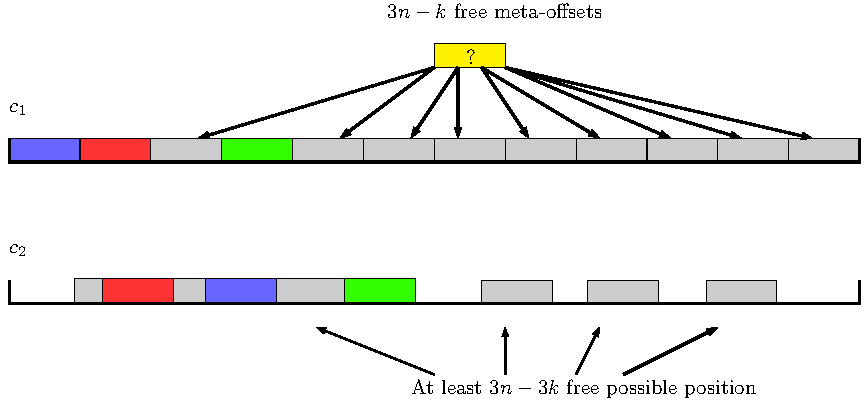
\includegraphics[width=0.9\textwidth]{ex3nt.pdf}
      \end{center}
      \caption{Times used in the period in $c_1$ and $c_2$, when scheduling the $4$th route in \metaoffset, with a period $P = 3n\tau$}
      \label{fig:metaoffset}
      \end{figure}


% 	\begin{algorithm}[H]
% 	\caption{Greedy assignment}
% 	\begin{algorithmic}
% 	\REQUIRE ${\cal R}_{\cal C}$, period $P$
% 	\ENSURE A P-periodic assignment in p $\leq P$, or FAILURE
% 	\STATE $T$ a table of the macro slots of size $\tau$ in the forward period.
% 	\STATE $L$ a list of free intervals in the backward period%$P2[P]$ slots backward period.
% 	\FORALL{source $s$ in S}
% 
% 	\FORALL{free intervals $[a,b]$ in $L$}
% 	\FORALL{ $a/\tau - \lambda(s) <j< b/\tau - \lambda(s)$ }
% 	\IF{ $T[j] == FREE$}
% 	\STATE $m_{s} \leftarrow j.\tau$
% 	\STATE $T[j] = USED$
% 	\STATE update $[a,b]$ in $L$
% 	\STATE BREAK
% 	\ENDIF
% 	\ENDFOR
% 	\ENDFOR
% % 	
% % 	\IF{No intervals are found for $s_i$}
% % 	\STATE return FAILURE
% % 	\ENDIF
% % 	\ENDFOR
% 
% 	\ENDFOR
% 
% 	\end{algorithmic}
% 	\end{algorithm}
	
This algorithm, contrarily to the previous one, may work well, even for loads higher than $1/3$.
In fact, experimental data in Section~\ref{sec:exp_PAZL} suggest that the algorithm finds a solution when the load is less than $1/2$.


\subsection{Compact Assignment}

In this section, we show how every bufferless assignment can be put into a canonical form.
We use that form to design an algorithm solving \pazl in fixed parameter tractable time ($\FPT$), with parameter $n$ the number of routes (for more on parametrized complexity see~\cite{downey2012parameterized}). This is justified since $n$ is small in practice, from $10$ to $20$ in our settings, and the other parameters such as $P$, $\tau$ or the weights are large.

Let $({\cal R},\omega)$ be a star routed network and let $A$ be a bufferless $(P,\tau)$ assignment.
We say that $A$ is \textbf{compact} if there is a route $r_0 \in \cal{R}$ such that the following holds: for all subsets $S\subset \cal{R}$ with $r_0 \notin S$, the bufferless assignment $A'$, defined by $A'(r) = A(r) - 1 \mod P$ if $r \in S$ and $A(r)$ otherwise, is not valid. In other words, an assignment is compact if for all routes $r$ but one, $A(r)$ cannot be reduced by one, that is either in $c_1$ or in $c_2$, there is a route $r'$ using the tics just before $r$. See Figure~\ref{fig:compact} for an example of a compact assignment, obtained by the procedure of the next proposition. 
  \begin{figure}
      \begin{center} 
      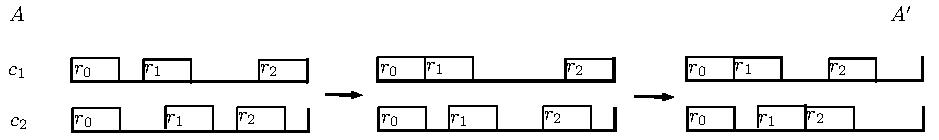
\includegraphics[width=\textwidth]{compacttoassignment.pdf}
      \end{center}
      \caption{Transformation of a bufferless assignment $A$ into a compact assignment $A'$, following the process of Proposition~\ref{prop:compactification}}
      \label{fig:compact}
      \end{figure}
\begin{proposition}\label{prop:compactification}
Let $N = ({\cal R}, \omega)$ be a star routed network. If there is a $(P,\tau)$-periodic bufferless assignment of $N$, then there is a compact $(P,\tau)$ assignment of $N$.
\end{proposition}
\begin{proof}
Consider $A$, a $(P,\tau)$-periodic bufferless assignment of $N$.
We describe an algorithm which builds a sequence $COMP_i$ of sets of routes and a sequence  
$A_i$ of valid bufferless assignments. For all $i \leq n$, the set $COMP_i$ has cardinal $i$ and satisfies  $COMP_{i-1} \subset COMP_i$

Let $r$ be an arbitrary route of ${\cal R}$ and $A_0 = A$, we set $COMP_0 = \emptyset$.
 For $i = 1$ to $n$, we choose a route $r$, denoted by $r_i$, as follows.
Let $A_{i} = A_{i-1}$. While there is no collision, for all routes $r \in {\cal R} \setminus COMP_{i-1}$, let $A_i(r) = A_i(r) - 1$. Then choose any route $r$ in ${\cal R} \setminus COMP_{i-1}$ such that setting $A_i(r) = A_i(r)-1$ creates a collision and let $r_i = r$. By construction, $A_i$ is a valid bufferless assignment, since it is modified only when no collision is created. We let $COMP_i = COMP_{i-1} \cup \{r_i\}$.

We prove by induction on $i$, that $A_i$ is compact when restricted to $COMP_{i}$.
We have $|COMP_1| = 1$, hence $A_1$ is compact over $COMP_1$. Let us consider $A_i$,
by induction hypothesis, since the offsets of routes in $COMP_{i-1}$ are not modified at step $i$ of the algorithm, $A$ is compact when restricted to $COMP_{i-1}$. 

 Consider $S \subseteq COMP_i$ which does not contain $r_0$. If $S$ contains
an element of $COMP_{i-1}$, then $S \setminus \{r_i\}$ is not empty and by compacity we cannot decrement all offsets of $S\setminus \{r_i\}$ without creating a collision. The same property is true for $S$. If $S = \{r_i\}$, then by construction of $r_i$ by the algorithm, removing one from $A_i(r_i)$ creates a collision. Hence, $A_i$ is compact restricted to $COMP_{i}$, which proves the induction and the proposition.
\end{proof}

We now present an algorithm to find a $(P,\tau)$ assignment by trying all compact assignments.

\begin{theorem}\label{th:FPT}
$\pazl \in \FPT$ over star routed networks when parametrized by the number of routes.
\end{theorem}
\begin{proof}
Let $N = ({\cal R},\omega)$ be a canonical star routed network and let $P$ be the period and $\tau$ the size of a datagram. For a given assignment and a route $r$ with offset $o_r$, by removing $o_r$ to all offsets, we can always assume that $o_r = 0$. By this remark and Proposition~\ref{prop:compactification}, we need only to consider all \emph{compact assignments} with an \emph{offset $0$} for the route $r_0$. We now evaluate the number of compact assignments and prove that it only depends on $n$ the number of routes to prove the theorem.

 We describe a way to build any compact assignment $A$ by determining its offsets one after the other, which gives a bound on their number and an algorithm to generate them all. We fix an arbitrary total order on ${\cal R}$. Let $r_0$ be the first route in this order, its offset is set to zero, and we let $S = \{r_0\}$,
 $S_1 = \{r_0\}$ and $S_2 = \{r_0\}$. $S$ represent the routes whose offsets are fixed, 
 offsets of unscheduled routes are chosen so that they follow a route of $S_1$ in $c_1$ or a route of $S_2$ in $c_2$.

 At each step, we add an element to $S$: let $r$ be the smallest element of $S_1$, if it is non-empty. Then, select any route $r' \in {\cal R} \setminus S$ 
 such that $o_{r'} = o_{r} + \tau$ does not create a collision (by construction $o_{r'} = o_{r} + \tau - 1$ does create a collision in $c_1$). Then, we update the sets as follows:
 $S = S \cup \{r'\}$, $S_1 = S_1 \setminus \{r\} \cup \{r'\}$ and $S_2 = S_2 \cup \{r'\}$. If 
 $S_1$ is empty, $r$ is the smallest element of $S_2$, and we set $o_{r'} = o_{r} + \tau + \omega(r,c_2) - \omega(r',c_2)$.
 We can also remove $r$ from $S_1$ (or from $S_2$ if $S_1$ is empty) without adding any element to $S$. The value of the offset of the route added to $S$ is entirely determined by the values of the offsets of the routes in $S$.

 Any compact assignment can be built by the previous procedure, if the proper choice of element to add is made at each step. Hence, this process generates all compact assignments. We now bound the number of compact assignments it can produce. When $|S| = i$, we can add any of the $n-i$ routes in ${\cal R} \setminus S$ to $S$. Hence, the number of sequences of choices of routes to add is $n!$ (but some of these sequences can fail to produce a valid assignment). We have not yet taken into account the steps at which an element is removed from either $S_1$ or $S_2$, without adding something to $S$. At each step of the algorithm, we can remove an element or not, there are at most $2n$ steps in the algorithm, hence there are at most $4^n$ sequences of such choices during the algorithm. As a conclusion, there are at most $4^nn!$ compact assignments.

The algorithm to solve \pazl builds every possible compact assignment in the incremental manner described here, and tests at each step whether, in the built partial assignment, there is a collision, which can be done in time linear in the size of $N$. Therefore, $\pazl \in \FPT$.
\end{proof}


We call the algorithm described in Theorem~\ref{th:FPT} \textbf{Exhaustive Search of Compact Assignments}
or \ESCA. The complexity of \ESCA is in $O(4^n n!)$. While a better analysis
of the number of compact assignments could improve this bound, the simple star routed networks with all arcs of weights $0$ has $(n-1)!$ compact assignments. Hence, to improve significantly on \ESCA, one should find an even more restricted notion of bufferless assignment than compact assignment.

To make \ESCA more efficient in practice, we make cuts in the search tree used to explore all compact assignments. Consider a set $S$ of $k$ routes whose offsets have been fixed at some point in the search tree. We consider the times used by these routes in $c_1$. It divides the period into $[(a_0,b_0), \dots, (a_{k-1},b_{k-1})]$ where the intervals $(a_i,b_i)$ are the times not used yet in $c_1$. Therefore, at most $\displaystyle{ \sum_{i=0}^{k-1} \lfloor(b_{i} -a_i)/\tau\rfloor}$ routes can still send a datagram through $c_1$. If this value is less than $n - k$, it is not possible to create a compact assignment by extending the current one on $S$, and we backtrack in the search tree. The same cut is also used for the contention point $c_2$. These cuts rely on the fact that the partial assignment is wasting bandwith by creating intervals which are not multiples of $\tau$. They significantly speed up \ESCA on instances of large load, which are also the longest to solve.



   \subsection{Experimental Evaluation}\label{sec:exp_PAZL}

   
  In this section, the experimental results of the three presented algorithms are compared.
   Notice that both \metaoffset and \shortestlongest are polynomial time algorithms but are not always able to find a solution, depending on the load or the size of the routes. On the other hand, \ESCA finds a solution if it exists, but works in exponential time in $n$. We compare the performance of the algorithms in two different regimes: routes are either short with regard to $\tau$, or unrestricted.

   \paragraph{Experimental Settings}


     The defaults parameters of all experiments in this article are derived from the C-RAN context~\cite{wang2017cloud} and summarized in the table of Figure~\ref{tab:params}: a tic corresponds to the sending time of $64$ Bytes of data on links of bandwidth $10$~Gbps. The datagrams are approximately of size $1.18$~Mbit, which corresponds to $2,500$ tics. 

     All experiments are done on synthetic networks generated randomly. We generate the physical fronthaul
     network, as represented in Figure~\ref{fig:star}, by drawing the size of each link according to some distribution which depends on the experiment. Then, the corresponding canonical star routed network is built from the generated fronthaul and the algorithms tested on it. 

     In the following experiments, we illustrate how well the algorithms work for different values of the load. To change the load, we choose to fix both parameters $\tau$ and $n$, and to modify the period $P$, which allows for a smooth control of the load and does not impact the execution time of the algorithms. In most experiments, we fix the number of routes to $n = 8$. In the case of fronthaul networks the period is one ms, that correspond to $20,000$ tics and thus a load of $0.95$ with eight routes.

     For all experiments of this paper, the code in C is available on the web page of one author\cite{webpage} under a copyleft license. The code has been run on a standard $2016$ laptop with a $2.2$~Ghz Intel Core i5 and the sources are compiled with gcc version 8.4.0. All experiments end in at most a few dozen seconds.

\begin{figure}
\begin{center}
\begin{tabular}{|c|c|c|}
\hline
Parameter& Value & Time in tics \\
\hline
Duration of a tic& $\simeq51$ns&1 tic\\
\hline
Datagram size ($\tau$)&  $1.18$~Mbit & $2500$ tics\\
\hline
Period ($P$)& $1$ms&$\simeq20,000$ tics\\
\hline
Bandwidth of links &  $10$~Gbps & -\\
\hline
Number of routes ($n$) & $8$ & -\\
\hline
\end{tabular}

\end{center}

\caption{Parameters of experiments on realistic network topologies}
\label{tab:params}
\end{figure}
    \paragraph{Short Routes}
      
    

 	 We first consider routes which are shorter than $\tau$: a datagram cannot be contained completely in a single arc which is common in our applications. We generate random star routed networks, by drawing uniformly at random the weights of the arcs of the fronthaul network in $[700]$, which corresponds to links of length less than $5$km between a BBU and an RRH.

     In the following experiment, we generate $10,000$ random instances of \pazl for a load of $1$ down to $0.4$. We represent, in Figure~\ref{fig:short}, the percentage of success of each algorithm as a function of the load. We make three experiments with $8$, $12$ and $16$ routes to understand the effect of the number of routes on the quality of our algorithms. A bound on the maximal success rate is given by the exhaustive search, which always finds a solution if there is one. 
       
      \begin{figure}[h]
      \begin{center}
	 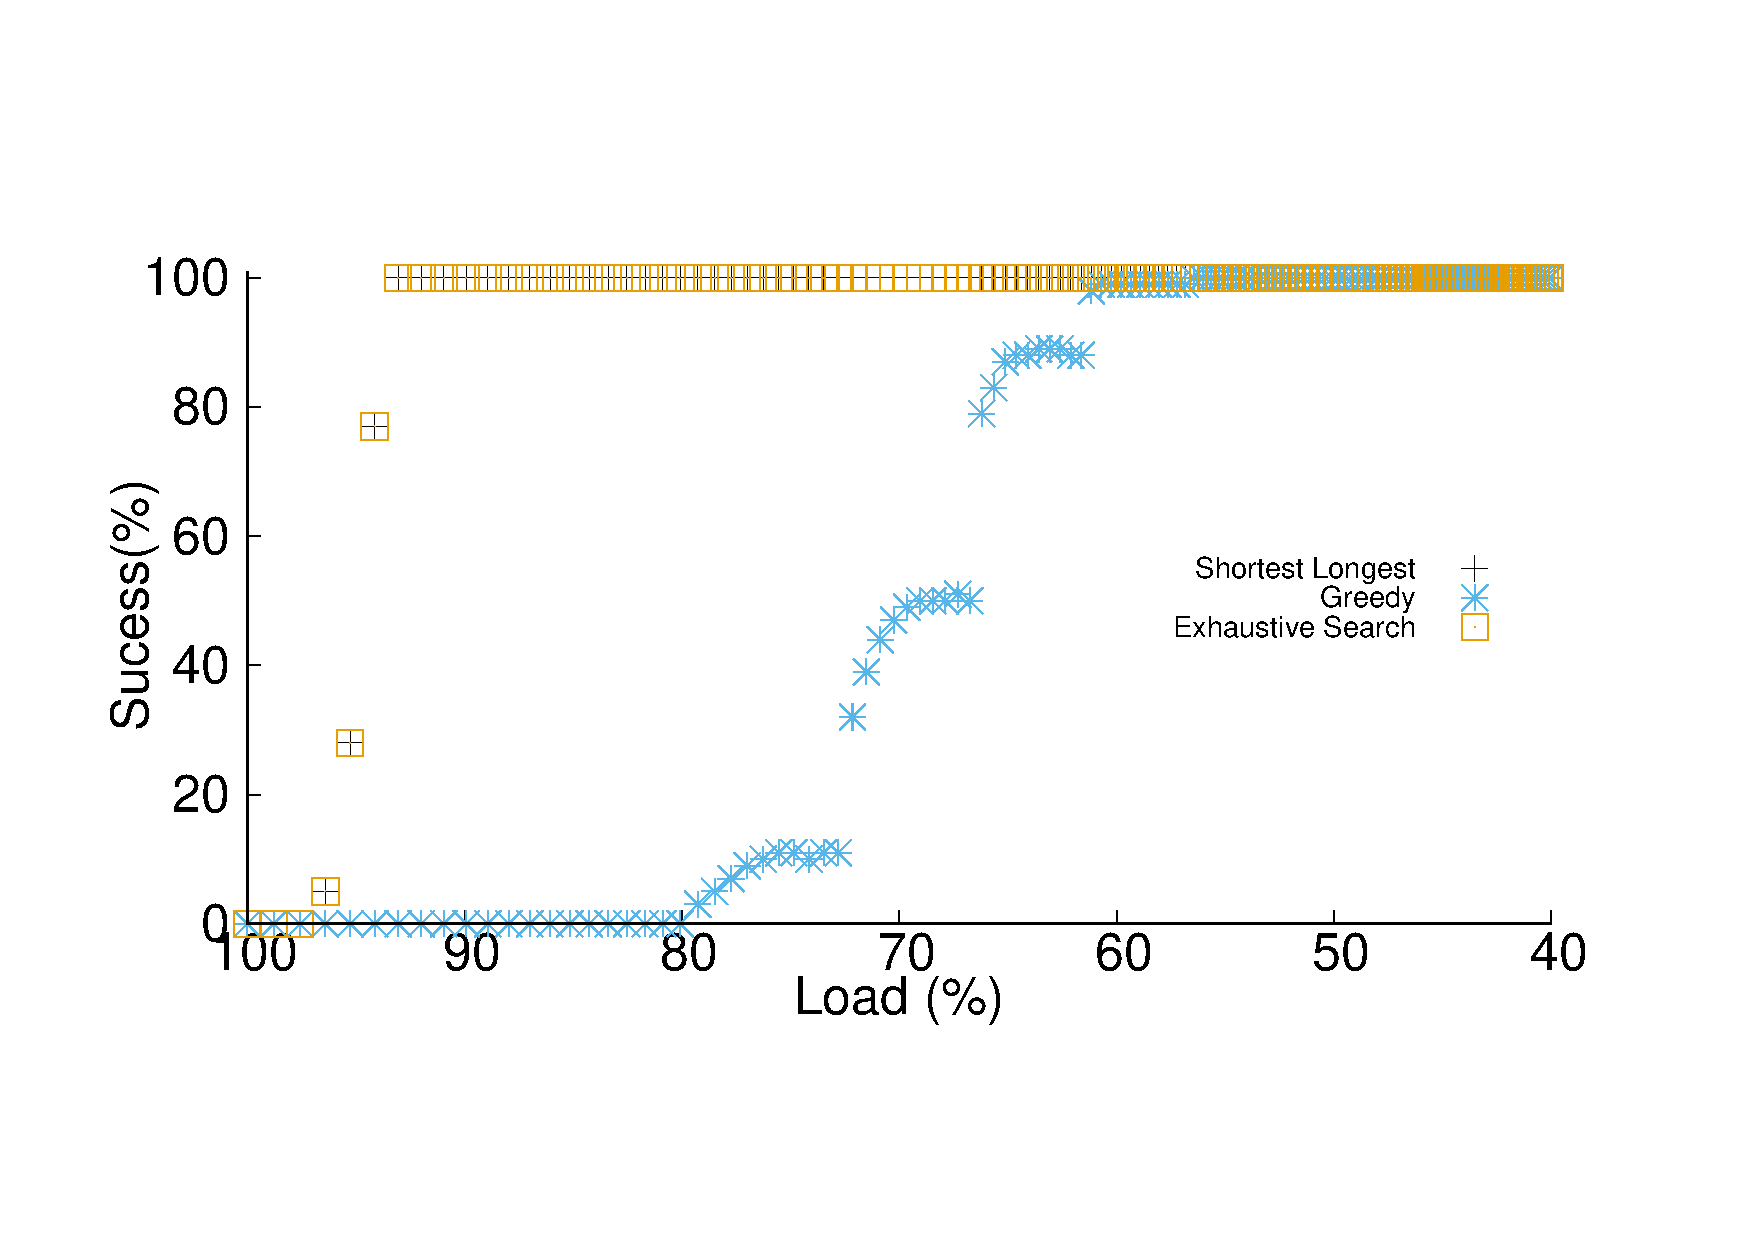
\includegraphics[width=0.9\textwidth]{pazlshort8.pdf}
\vspace{1cm}

	 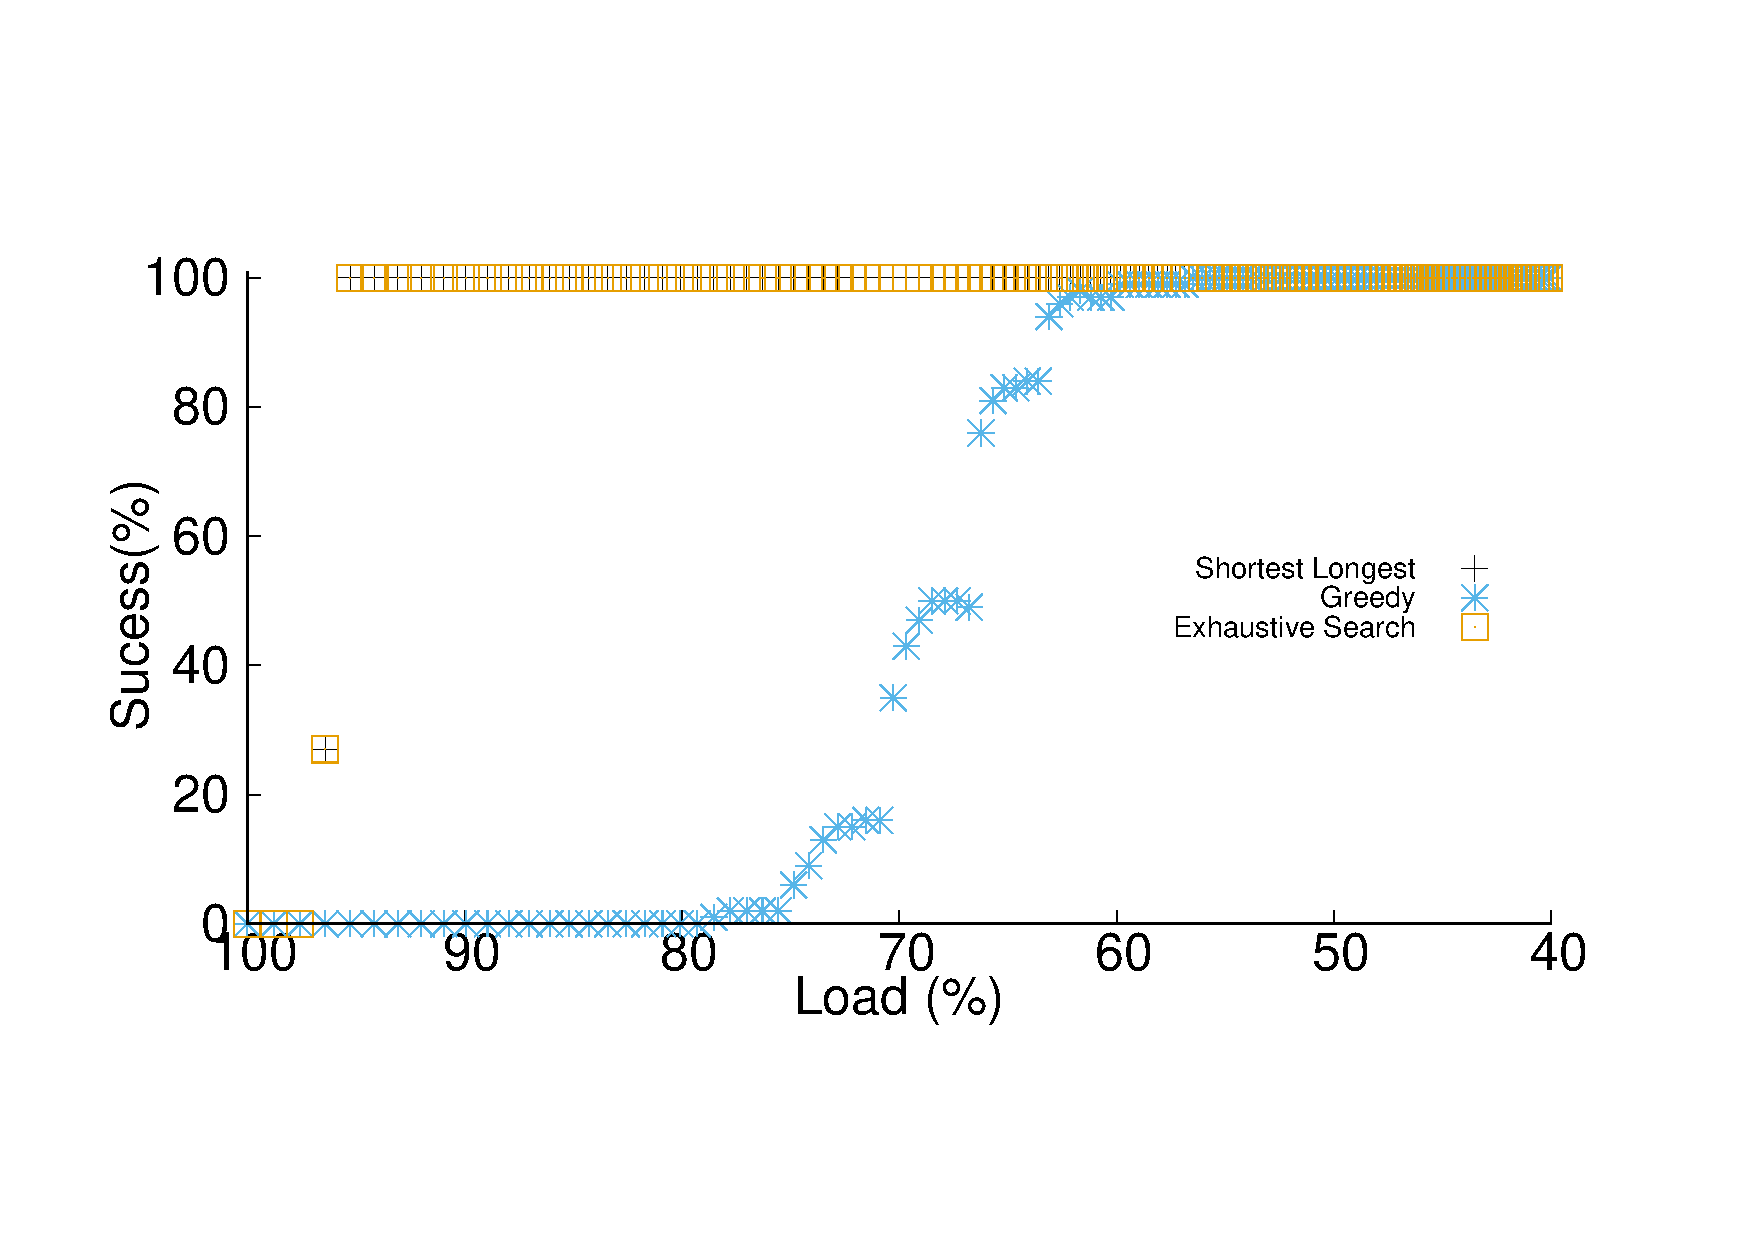
\includegraphics[width=0.45\textwidth]{pazlshort12.pdf}
	 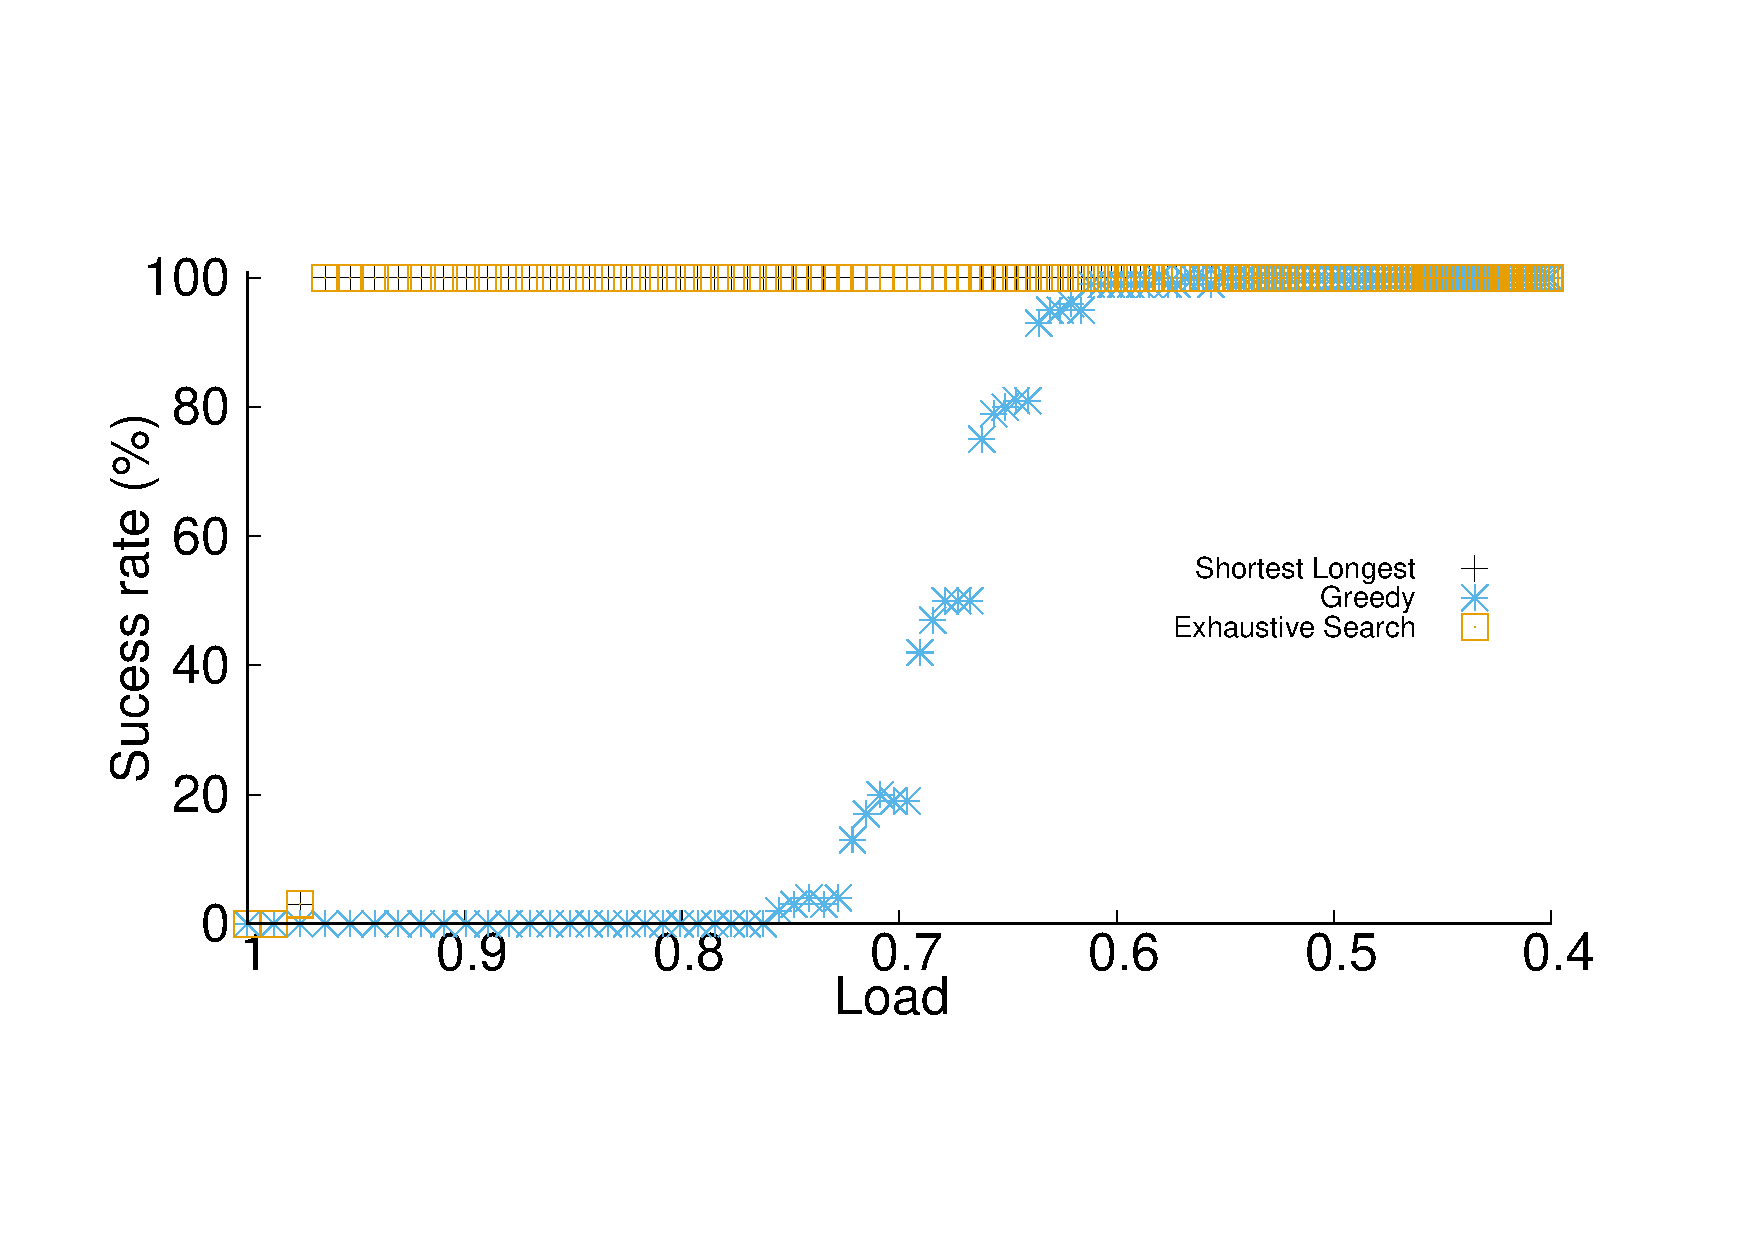
\includegraphics[width=0.45\textwidth]{pazlshort16.pdf}
      \end{center}
      \caption{Success rate of the three algorithms solving \pazl, for short routes and $8$ routes (top), $12$ routes (bottom left) and $16$ routes (bottom right)}\label{fig:short}
      \end{figure}

      First, \ESCA finds a solution even when the load is high. It justifies the idea to look for a bufferless assignment, in this short routes regime. 
      It seems that increasing the number of routes makes the exhaustive search even more efficient, meaning that the more the routes, the more instances have a bufferless assignment. 
      Second, \shortestlongest is as good as the exhaustive search. While it was expected to be good with short routes (see Proposition~\ref{prop:SL}), it turns out to be optimal for all the random star routed networks we have tried. Therefore, we should use it in practical applications with short routes, instead of the exhaustive search, which is much more computationally expensive. 

      Finally, the greedy algorithm seems to always work when the load is less than $1/2$ and has a good probability to work up to a load of $2/3$, which is twice better than the theoretical bound. The performance of \metaoffset seems to depend on the load only and not on the number of routes. There are discontinuities in the probability of success at several loads, which seem to smooth out when the number of routes increases. It can be explained by the fact that \metaoffset becomes better when decreasing the load makes the number of available meta-offsets larger. The number of meta-offsets increases when $\tau$ is added to the period, which is more frequent when there are more routes.
      
        \paragraph{Long routes}
      
      We now want to understand the performance of these algorithms when the length of the routes is unbounded. In this experiment we fix the number of routes to eight and the weights of the arcs of the fronthaul network are drawn following a uniform distribution in $[P]$. We represent in Figure~\ref{fig:long} the percentage of success of each algorithm computed from $10,000$ random instances, for load from $1$ down to $0.4$.
\begin{figure}[h]

       \begin{center}
      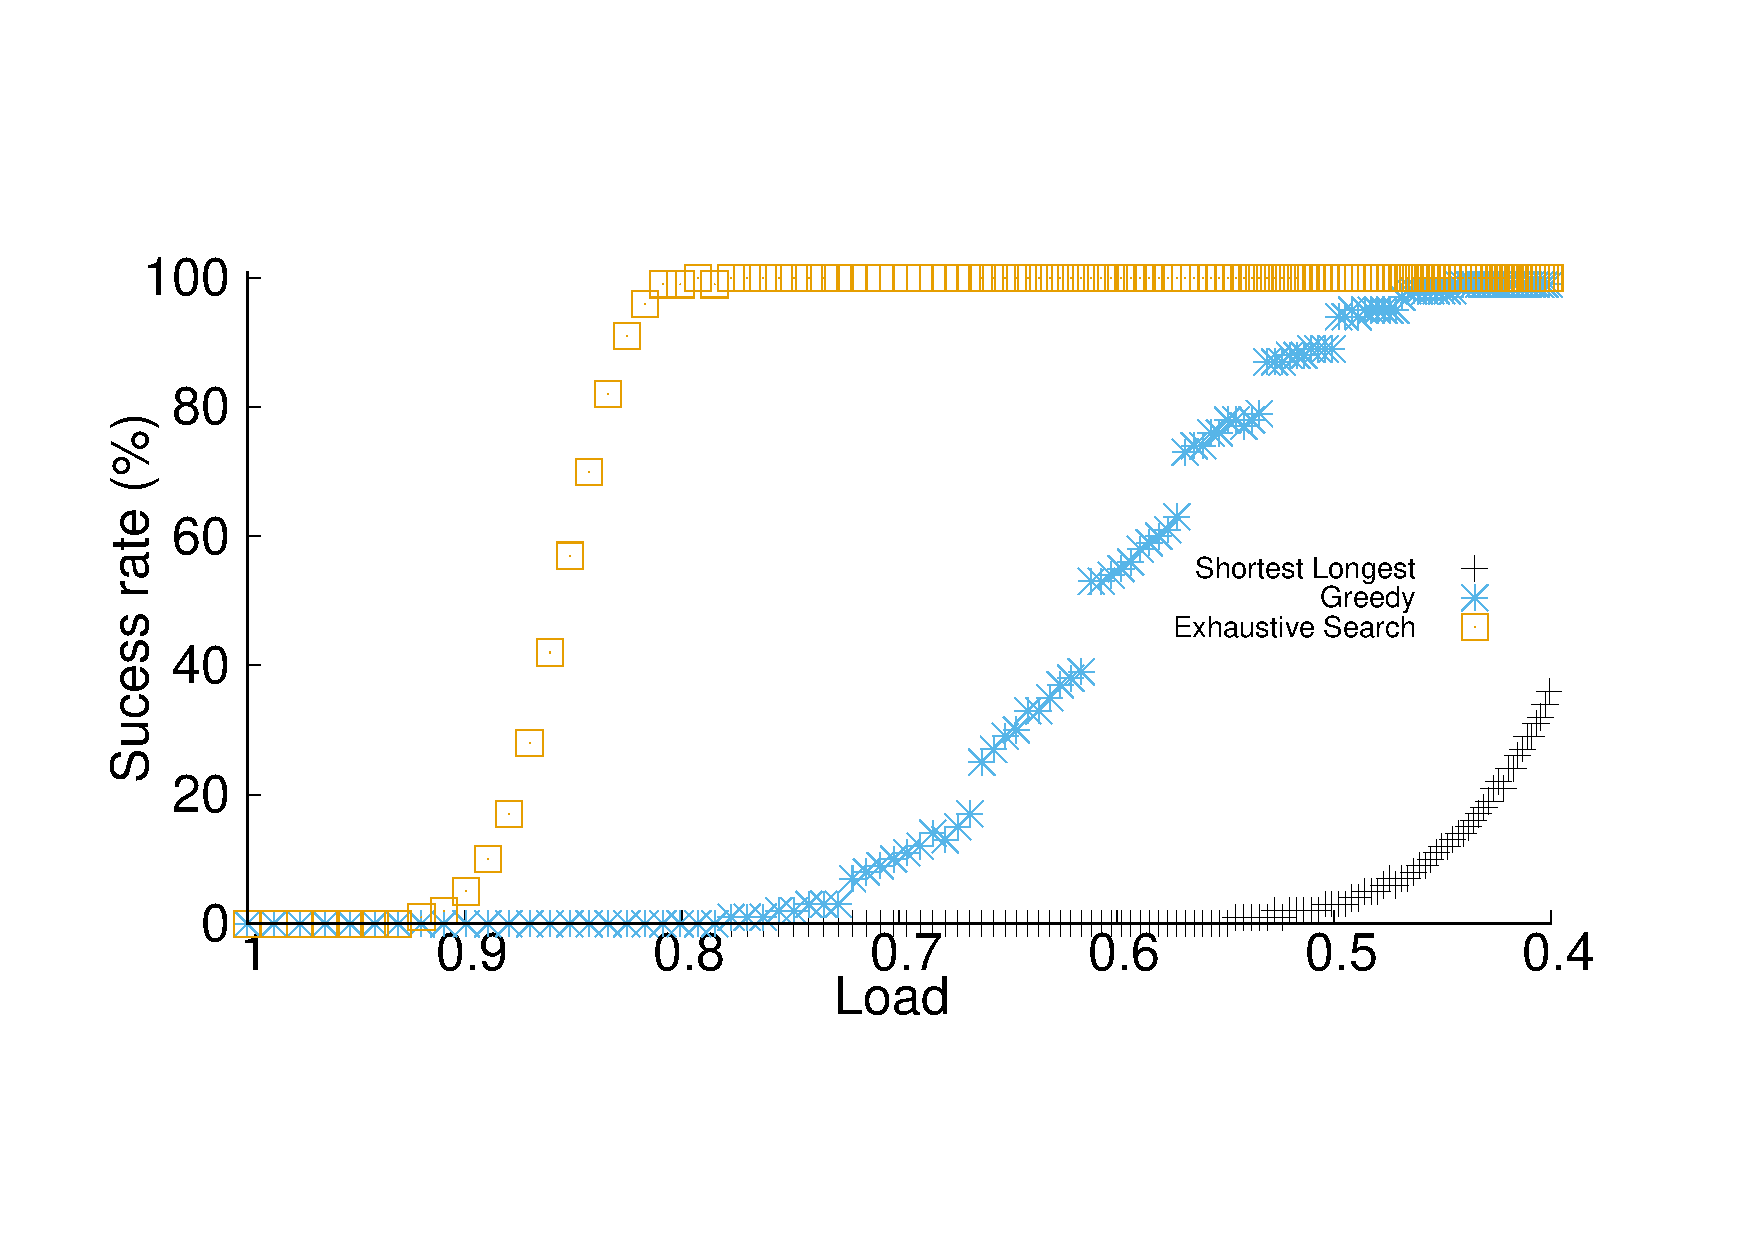
\includegraphics[width=0.9\textwidth]{echec_longues.pdf}
      \end{center}
        
      \caption{Success rate of the three algorithms solving \pazl, for $8$ routes of arbitrary length}\label{fig:long}
     \end{figure}
      
       In this regime, the performances of \shortestlongest are abysmal because it depends on the difference of size between the longest and the smallest route, which is large here.  Algorithm \metaoffset has a performance not far from the short routes regime, which is expected since it does not directly depend on the size of the route. 
      
       When the load is larger than $0.5$, the \ESCA finds more solutions than \metaoffset which justifies its use. However, for load larger than $0.8$ there are instances for which there are no solutions to \pazl. It means that with long routes and high load, looking for a bufferless assignment is far too restrictive. This justifies the design of algorithms for the general \pall problem, which we present in the next section. We will test them on $8$ long routes and a load between $1$ and $0.8$, parameters for which, as shown here, there are not always a bufferless assignment.
      
       The computation time of \ESCA is bounded by $O(4^nn!)$ as shown in Theorem~\ref{th:FPT}, but it can be much better in practice, either because it finds a solution quickly or because a large part of the tree of compact assignments is pruned during the algorithm. We study the evolution of the running time  of the algorithm when $n$ grows in the following experiment. The weights of the arcs are drawn following a uniform distribution in $[P]$ and the load is set to $0.95$.  The table of Figure~\ref{fig:table} shows the time before \ESCA ends, for $8$ to $16$ routes, averaged on $100$ random star routed networks. This shows that for less than $20$ routes, which corresponds to all current topologies, the algorithm is efficient enough, but we should improve it further to work on more routes.
       
             \begin{figure}[h]
         \begin{center}
         \begin{tabularx}{\textwidth}{|l|X|X|X|X|X|}
    \hline
   $n$ & $8$ & $10$& $12$&$14$& $16$\\
    \hline
   Time (s) & $6.10^{-5}$&$8.10^{-4}$&$2.10^{-2}$& $0.4$& $11$\\
    \hline
      \end{tabularx}
      \end{center}
      \caption{Running time of \ESCA, averaged over 100 random instances}
      \label{fig:table}
      \end{figure}
      
         \section{Solving \texttt{PALL} on Star Routed Networks}\label{sec:PALL}
    
    In this section, we consider the more general \pall problem on star routed networks. The datagrams are allowed to wait in the BBUs to yield more possible assignments. Hence, we allow the process time of a route to be greater than the length of the route, but it must be bounded by its deadline.


	\subsection{Simple Star Routed Networks}
		

	Often in real networks, the lengths of the routes are not arbitrary and we may exploit that to solve \pall easily. For instance, all the weights on the arcs $(c_1,c_2)$ are the same if all the BBUs are in the same data center and all datagrams require the same time to be processed in the BBUs.
    Finding an assignment in that case is trivial: send all datagrams so that they follow each other without gaps in $c_1$. In the corresponding canonical routed network, one can set $o_i = i\tau$.  Since all arcs $(c_1,c_2)$ are of weight zero in this case, the intervals of time used in $c_2$ are the same as for $c_1$ and there is no collision in $c_2$.

	Another possible assumption would be that all deadlines are larger than the longest route, which happens when all RRHs are at almost the same distance to the shared link.

	 \begin{proposition}\label{prop:asym}
	Let $N = ({\cal R}, \omega)$ be a canonical star routed network with $n$ routes, let $P \geq n\tau$ and let $d$ be a deadline function. Let $r_{n-1}$ be the longest route, and assume that for all $r\in {\cal R}$, $d(r) \geq \lambda(r_{n-1})$. Then, there is a $(P,\tau)$ assignment for $N$ and $d$ and it can be built in time $O(n)$.
	 \end{proposition}
      \begin{proof}
       The idea is to set the waiting times of all routes so their datagrams behave exactly as the datagram of $r_{n-1}$. The offset of the route $r_i$ is set to $i\tau$, which ensures that there is no collision in $c_1$ as soon as $P \geq n\tau$. The waiting time of the route $r_i$ is $w_i = \lambda(r_{n-1}) - \lambda(r_{i})$.
        
    The time at which the datagrams of $r_i$ arrives in $c_2$ is $t(r_i, c_2) = w_i + i\tau + \lambda(r_{i})$. Substituting $w_i$ by its value, we obtain $t(r_i, c_2) =  i\tau + \lambda(r_{n-1})$.
    Hence, there is no collision in $c_2$. We denote by $A$ the defined assignment. By definition of the transmission time, we have $TR(r_i,A) = w_i + \lambda(r_i) = \lambda(r_{n-1})$. By hypothesis, $d(r_i) \geq \lambda(r_{n-1})$, which proves that the assignment respect the deadlines.

	Finally, the complexity is in $O(n)$ since we have to find the maximum of the length of the $n$ routes, and the computation of each $w_i$ is done by a constant number of arithmetic operations.
     \end{proof}
     
    
     \subsection{Two Stages Approach}
     
      We may decompose an algorithm solving \pall on a star routed network in two parts: first set all the offsets of routes so that there is no collision in $c_1$ and then knowing this information find waiting times so that there is no collision in $c_2$ while respecting the deadlines. 
      
     First, we give several heuristics to choose the offsets, which are experimentally evaluated in Section~\ref{sec:resultsPALL}. 
     For the first two heuristics, we need to define the margin. The \textbf{margin} of a route $r$ in a routed network $N$, with a deadline function $d$, is $ d(r) - \lambda(r)$. The margin is a bound on the waiting time of a route in a valid assignment.

     For all presented algorithms, we assume that the star routed network is given in canonical form. 
      We send the datagrams through $c_1$ in a compact way (no gap between datagrams). It means that for $n$ routes, denoted by $r_0, \dots, r_{n-1}$, the offsets are $o_i = \sigma(i) \times \tau$, for some permutation $\sigma \in \Sigma_n$. We consider the following orders $\sigma$: 
	
	\begin{itemize}
	 \item Decreasing Margin (DM): Decreasing order on the margin of the routes.
	 \item Increasing Margin (IM): Increasing order on the margin of the routes. 
	 \item Decreasing Arc Weight (DA): Decreasing order on the weight of the arcs $(c_1,c_2)$.
	 \item Increasing Arc Weight (IA): Increasing order on the weight of the arcs $(c_1,c_2)$. This sending order yields a $(P,\tau)$ assignment in which the waiting times are zero, if the period is large enough (see Proposition \ref{prop:SL}).
	\end{itemize}

    Alternatively, we propose to fix the offsets of the routes according to some random order.
    If we pack the datagrams as previously, we call Random Order (RO), the heuristic of choosing an order
    uniformly at random. We may also allow some time between two consecutive datagrams in $c_1$. The order of the routes in $c_1$ is still random and we consider two variations. Either the time between two datagrams in $c_1$ is random and we call this heuristic Random Order and Random Spacing (RORS) or the time between two consecutive datagrams is always the same and we call this heuristic Random Order and Balanced Spacing (ROBS).
 	
 	We call \textbf{W}aiting \textbf{T}ime \textbf{A}ssignment or \wta the problem \pall where the offsets of the routes are also given as input. A solution to \wta
 	is a valid assignment such that the offsets coincide with those given in the instance. 


 \bigskip

      \noindent {\bf Waiting Time Assignment }(\wta)

      \noindent {\bf Input:}  A routed network $N=({\cal R},{\cal B},\omega)$, integers $P$ and $\tau$, a deadline function $d$ and an offset $o_r$ for each route $r \in {\cal R}$.
      
      \noindent {\bf Question:} Does there exist a valid $(P,\tau)$ assignment $A$ of $N$ such that for all $r \in {\cal R}$, $TR(r,A) \leq d(r)$ and $A(r) = (o_r,w_r)$?
      \bigskip


   In the rest of the section, we study different methods to solve \wta either by polynomial time heuristics or by an FPT algorithm. The methods to solve \wta are then combined with the heuristics we have described to fix the offsets of the routes, which yields an algorithm solving \pall.  
   
   \subsection{Greedy Scheduling of Waiting Times}

   We consider an instance of the problem \wta, constitued of a canonical routed network, a deadline function and an offset for each route. The \textbf{release time} of a route is defined as the first time its datagram can go through $c_2$: for a route $r$ with offset $o_r$, it is $\lambda(r,c_2) + o_r$, it is the same as the arrival time in $c_1$, $t(r,c_1)$, and it is fixed in an instance of \wta.

    The first algorithm we propose to solve \wta is a greedy algorithm that sets the waiting times, by prioritizing the routes with the earliest deadline to best satisfy the constraints on the process time. Since the network is in canonical form, $\omega(r,t_r) = 0$ for all routes $r$, thus choosing the earliest deadline is equivalent to choosing the route with the smallest margin.
    
    We call the algorithm \greedydeadline, and it works as follows. Set $t=0$ and $U = \cal{R}$. While there is a route in $U$, find $s \geq t$ the smallest time for which there is $r \in U$ with a release time lower or equal to $s$. If there are several routes in $U$ with a release time lower or equal to $s$, then $r$ with the smallest deadline is selected and we set $w_r = s - \lambda(r,c_2)$, $t = s + \tau$ and $ U = U \setminus \{r\}$.

    This algorithm does not take into account the periodicity, which may create an assignment that is not valid. Let $r_0$ be the first route selected by the algorithm, then $t_0 = t(r_0,c_2)$ is the first time at which a datagram go through $c_2$.
	Then, if all routes $r$ are such that $t(r, c_2) \leq t_0 + P - \tau$, 
	then by construction, there is no collision on the central arc.
      However, if a route $r$ has $t(r, c_2)$ larger than $t_0 + P - \tau$, since we consider everything modulo $P$ to determine collision, it may collide with another route. Therefore, we correct \greedydeadline by this simple modification: $s \geq t$ is the smallest time for which there is $r \in U$ with a release time lower or equal to $s$ \emph{such that there is no collision if a datagram goes through $c_2$ at time $s$}. This rule guarantees that if \greedydeadline succeeds to set all waiting times, it finds a solution to \wta, as illustrated in Figure~\ref{fig:greedydeadline}. However, it can fail to find the value $s$ at some point because the constraint on collisions cannot be satisfied. In that case \greedydeadline stops without finding a solution.
    
    \begin{figure}
          \begin{center}
   \begin{tabularx}{0.9\textwidth}{|c|X|X|X|X|X|X|}
    \hline
     Route& $0$ & $1$ & $2$& $3$ & $4$\\
    \hline
    Deadline & $10$ &$15$&$5$&$7$&$32$\\
    \hline
     Release time & $0$ &$2$&$3$&$16$&$17$\\
    \hline
    Waiting time & $0$ &$5$&$1$&$0$&$15$\\
    \hline
      \end{tabularx}
      
      \vspace{1cm}
      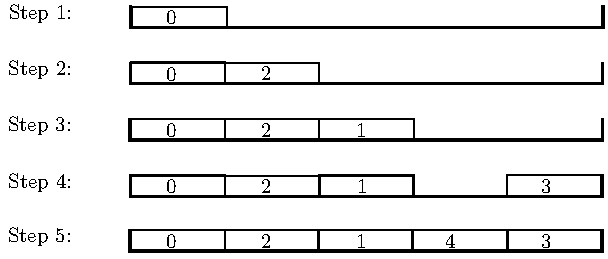
\includegraphics[width=0.9\textwidth]{examplegreedy.pdf}
      \caption{A run of \greedydeadline with $P = 20, \tau = 4$.}
           \label{fig:greedydeadline}
      \end{center}
      
    \end{figure}

    %Algorithm~\ref{alg:GD} is the formal description of the previous algorithm. 
    % The function  min\_non\_assigned(eligible\_time) returns the non assigned route with the smallest time eligible time. The function update(t,free\_intervals) removes an interval of size $\tau$ beginning at t, which correspond to the datagram,  from free\_intervals.
     
    %  \begin{algorithm}\label{alg:GD}
    % \caption{ Greedy deadline ({\bf GD}) }
    % \begin{algorithmic}
    % \REQUIRE A routed network $(G,{\cal R})$, a period $P$, packet size $\tau$, the deadlines $d_i$, the offsets $m_i$
    % \ENSURE $(P,\tau)$-periodic assignment of $(G,{\cal R})$, or failure
    %\STATE  ${\cal H} \leftarrow$ empty set //{\em set of eligible routes with their deadline}
     %   \STATE  free\_ intervals $\leftarrow$ [0,$P$] //{\em list of intervals of free slots}
   
    % \FORALL{route $r_{i}$}
%      \STATE  deadline[$r_i$]  $\leftarrow$  $m_{i} + T_{max} - \Omega(s_i,c_s)$
     %\STATE  eligible\_time[$r_i$] $\leftarrow$ $m_{i} +  \lambda(r_i) + \Omega(c_t,t_i)$
     %  \ENDFOR
       
     %  \WHILE{There is some non-assigned routes}
      % \IF{${\cal H}$ is empty}
     %  \STATE $r_i$ $\leftarrow $ min\_non\_assigned(eligible\_time)
     %  \STATE insert(${\cal H}$,$r_i$,$d_i$).
     %  \ENDIF
      
      % \STATE $r \leftarrow $ extract\_min(${\cal H}$)
      % \STATE t $\leftarrow$ next\_free\_interval(free\_intervals, t) //{\em if there is no more free interval of size $\tau$, the algorithm fails}
      % \STATE $w_i \leftarrow$ t - eligible\_time[$r_i$]
      % \STATE update(t,free\_ intervals)
      % \STATE t $\leftarrow$ t + $\tau$
      % \FORALL{routes $r_i$ with  eligible\_time[$r_i$] $\leq$ t}
 	 %	\STATE insert(${\cal H}$,$r_i$).
      % \ENDFOR
      % \ENDWHILE
     %\end{algorithmic}
     %\end{algorithm}

   


    The complexity of \greedydeadline is in $O(n\log(n))$, using the proper data structures. The set of routes $\cal{R}$ must be maintained in a binary heap to be able to find the one with the smallest deadline in time $O(\log(n))$. To deal with the possible collisions, one maintains a list of the intervals
    of time during which a datagram can go through $c_2$. When the waiting time of a route is fixed, an interval is split into at most two intervals in constant time. During the whole algorithm, each element of this list is used at most twice either when doing an insertion or when looking for the next free interval. Hence, the time needed to maintain the list is in $O(n)$. 
  
     \subsection{Earliest Deadline Scheduling}\label{sec:wtaheuristic}
     
     
     If we forget periodicity, the problem \wta is similar to the classical \emph{single processor scheduling} problem: Given a set of tasks with \emph{release times} and \emph{deadlines}, schedule all tasks on a single processor, that is choose the time at which they are executed, so that no two tasks are scheduled at the same time. A task is always scheduled after its release time and it must be dealt with before its deadline. This scheduling problem can be solved in polynomial time when \emph{jobs are unit-time}~\cite{simons1978fast}, that is when they are run for the same time.
     The problem is $\NP$-complete~\cite{lenstra1977complexity} when the running times of the jobs are different. Several algorithms solve this problem
     for all tasks with the same running time~\cite{simons1978fast,carlier1979probleme,garey1981scheduling} and the fastest one is in time $O(n\log(n))$, where $n$ is the number of jobs.
     Note that all algorithms also minimize the makespan, that is the time at which the last job is scheduled, a property useful for our work. 

     %They all build on 
     %a greedy routine similar to \greedydeadline. However, when it fails because a job finishes after its deadline, it changes the schedule of the last jobs to find a possible schedule for the problematic job. The change in the scheduling is so that the algorithm cannot fail on the same job a second time except if there is no solution, which proves that the algorithm is in polynomial time. 
     
     The problem \wta is the same as the single processor scheduling problem with unit-task but adding constraints arising from
     the periodicity: The tasks are the routes, the size of a datagram is the running time of a task, 
     the release time and the deadline are the same in both models, when we assume the star routed network to be canonical.
	 Let us call \textbf{M}inimal \textbf{L}atency \textbf{S}cheduling, denoted by \MLS, the algorithm which transforms an instance of \wta into an instance of the described scheduling problem to solve it in time $O(n\log(n))$ using the algorithm of~\cite{garey1981scheduling}.
     
     Recall that $t(r,c_2)$ is the time at which the datagram of $r$ goes through $c_2$. Let us denote by $t_{min}$ and $t_{max}$ the smallest and largest value of $t(r_i,c_2)$ for all $i \in[n]$. When \MLS finds an assignment $A$, it always satisfies $PT(r) \leq d(r)$ for all $r$. Moreover, by construction \MLS schedules the datagrams without collision if we forget about the periodicity (each route send only one datagram). Let us assume that $t_{max}- t_{min} \leq P -\tau $, then all datagrams go through $c_2$ during a interval of time less than $P$. Hence, when we compute potential collisions modulo $P$, all the relative positions of the datagrams stay the same which implies there is no collision. However, if $t_{max}- t_{min} > P -\tau $, then computing $t(r_i,c_2)$ modulo $P$ for all $i$ may reveal some collisions. Since the scheduling algorithm minimizes $t_{max}$, it tends to find  small values for $t_{max} - t_{min}$ and \PMLS may succeed in finding a valid assignment (as shown in Section~\ref{sec:resultsPALL}), but not for all instances. 
     
     We now present a variant of the previous algorithm, that we call
     \textbf{P}eriodic \textbf{M}inimal \textbf{L}atency \textbf{S}cheduling, denoted by \PMLS. The aim is to deal with the periodicity, by modifying the instance without changing the assignments, so that there is a better chance of finding a solution with $t_{max}- t_{min} \leq P -\tau $.  If an instance has a valid assignment, we can guarantee that one route has a waiting time zero in some valid assignment. 
     
      Recall that $t(r,c_1)$ is the release time of $r$. Algorithm \PMLS runs, for each route $r \in \cal{R}$, the algorithm \MLS on an instance defined as follows. Subtract $t(r,c_1)$ to all the release times and deadlines of the routes, to obtain an equivalent problem. Therefore, $t(r,c_1)$ is zero in the instance we build and the waiting time $w_r$ is set to zero. Hence, the datagram of $r$ goes through $c_2$ at time $0$ and $t_{min} = 0$.
     Then, as in Proposition~\ref{prop:canonical}, the instance is modified so that all release times are in $[P-\tau]$. Each release time $t(r_i,c_1)$ is replaced by $t(r_i,c_1) \mod P$ and $d(r_i) = d(r_i) - (t(r_i,c_1) - (t(r_i,c_1) \mod P))$. Furthermore, if the release time of a route $r$ is between $P-\tau$ and $P$, we set it to $0$ and $d(r) = d(r) - P$.  The deadline of each route is set to the minimum of its deadline and $P - \tau$. Hence, if \MLS finds a solution for such a modified instance, by construction of the instance, we have $t_{max} \leq P -\tau $. Since $t_{min} = 0$, the assignment is valid. Algorithm \PMLS returns the first assignment it finds when running \MLS for some $r \in \cal{R}$.

     The instance of \wta we have defined in this transformation is equivalent 
     to the original instance, except we have fixed the waiting time of 
     $r$ to be zero. If there is some valid assignment, then at least one route has waiting time zero. Hence, when \MLS finds an assignment, \PMLS also finds one. Algorithm \MLS is used at most $n$ times, thus the complexity of \PMLS is in $O(n^2\log(n))$. Note that \PMLS is a heuristic and may fail to find a solution even if it exists. It is the case when, for the $n$ modified instances, there is no solution with times $t(r_i,c_2)$ using an interval of time less than $P$ in $c_2$. 



%     \begin{algorithm}[H]
%     \caption{ Minimized Scheduling Periodic (MSP)}
%     \begin{algorithmic}
%     \REQUIRE A routed network $(G,{\cal R})$,a period $P$, packet size $\tau$, $ T_{max}$, the offsets $m_i$
%     \ENSURE $(P-\tau)-$periodic assignment of $(G,{\cal R})$, if it exists
%   
%     \FORALL{route $r_{t_i}$}
%     \STATE  $w_i \leftarrow 0$
%     \STATE period-end $\leftarrow m_{s_i} + \lambda(r_{s_i}) + t(c_t,r_{t_i}) + P$
%     \FORALL{route $r_{t_j}$}
%     \STATE deadline-route$ \leftarrow m_{s_j} + T_{max}-t(c_s,r_{s_j})$
%     \STATE $deadline \leftarrow$ min(deadline-route,period-end)
%     \ENDFOR
%     
%     \STATE Call (MS)
% 
%     
%     \ENDFOR
% 
%     \STATE return the best $(P,\tau)$-periodic assignment, or FAILURE
% 
%     \end{algorithmic}
%     \end{algorithm}

\subsection{FPT algorithms for \texttt{WTA} and \texttt{PALL}}

As a warm-up, we give a simple FPT algorithm for \wta which is practical,
and then we build on it to give a more complicated FPT algorithm for \pall. Unfortunately, the dependency on $n$ the number of routes in the second algorithm is yet too large to be useful in practice. 

\begin{theorem}\label{th:braFPT}
$\wta \in \FPT$ over star routed networks when parametrized by the number of routes.
\end{theorem}
\begin{proof}
 Consider an instance of \wta, which is given as a release time and a deadline for each route.
 We show that we can build a set of instances such that one of these instances has a valid assignment if and only if the original instance has a valid assignment.

  As for \PMLS, for each route $r$, we consider the instance where $r$ has release time and waiting time zero ($t(r,c_1) = w_r = 0$). The release times and deadlines of all routes are modified so that all release times are less than $P$ as in the transformation described for \PMLS. If there is an assignment such that $t_{max} < P-\tau$, then the periodicity does not come into play for this assignment and the algorithm \MLS will find the assignment as explained in Section~\ref{sec:wtaheuristic}.

 If there is a valid assignment for an instance with the previously stated properties,
 then there is a valid assignment satisfying for all $i$, $t(r_i,c_2) \leq 2P - \tau$.  
 Indeed, if there is a $i$ such that $t(r_i,c_2) \geq 2P$ in an assignment, then we have 
 $w_i = t(r_i,c_2) - \lambda(r_i,c_2) \geq P$. Hence, we can set $w_i = w_i -P \geq 0$ and we still have 
 a valid assignment. Moreover, for all $r_i \neq r$, it is not possible that $2P-\tau < \lambda(r_i,c_2) \leq 2P$, since it implies a collision between $r$ and $r_i$.
 

From an instance $I$, with the properties of the first paragraph, we define a new instance $I'$ whose valid assignments are a subset of the ones of $I$. Moreover, one of the valid assignments of $I'$ satisfies that, for all $i \in [n]$, $t(r_i,c_2) \leq P - \tau$ and is thus found by \MLS. 
Let us now consider $A$ a valid assignment of $I$, we can assume that, for all $i \in [n]$, $t(r_i,c_2) \leq 2P - \tau$. Let $S$ be the set of routes $r_i$ such that  $P - \tau < t(r_i,c_2) \leq 2P - \tau$. The instance $I'$ is defined by changing, for all route $r \in S$, $t(r,c_1)$ and $d(r)$ to $t(r,c_1) - P$ and $d(r) - P$. Then, by construction $A$ is also a valid assignment of $I'$. Assignment $A$ as a solution of $I'$, satisfies $t(r_i,c_2) \leq P - \tau$ for all $i\in [n]$. 

The FTP algorithm is the following: for each route $r$ build a modified instance as in $\PMLS$.
Then, for each subset $S$ of routes, remove $P$ to the release time and the deadline of each route in $S$ and run \MLS on the instance so modified. If there is a valid assignment, then we have proved that there is some $S$, such that the instance built from $S$ has a valid assignment with $t(r_i,c_2) \leq P - \tau$ for all $i\in [n]$. Hence, \MLS finds a valid assignment for this instance.
\end{proof}

The algorithm of Theorem~\ref{th:braFPT} has a complexity of $O(2^nn^2\log(n))$. If we consider some valid assignment, the routes $r$ with $t(r,c_2) > P$, must satisfy $t(r,c_2) > P + \tau$ to avoid collision with the first route. Hence, the deadline of these routes must be larger than $P + \tau$. These routes are exactly those that must be put in $S$, hence we can enumerate only the subsets of routes with a deadline larger than $P + \tau$. In practice, only $k$ routes have a deadline larger than $P + \tau$ with $k << n$, and we need only to consider $2^k$ subsets. Let us call this algorithm \textbf{A}ll \textbf{S}ubsets \PMLS, and let us denote it by \ASPMLS.


\begin{theorem}\label{th:pallFPT}
$\pall \in \FPT$ over star routed networks when parameterized by the number of routes.
\end{theorem}
\begin{proof}
 Consider an instance of \pall with a valid assignment. We characterize such a valid assignment by a set of necessary and sufficient linear equations and inequations it must satisfy.  These conditions are expressed on the values $t(r,c_1)$ and $t(r,c_2)$ and choosing these values is equivalent to choosing the offsets and the waiting times, that is choosing an assignment.

First, we assume the star routed network is canonical. Hence, there is a valid assignment $A$, such that for all routes $r \in \cal{R}$, $0 \leq t(r,c_1) < P -\tau$ and $0 \leq t(r,c_2) < 2P-\tau$. 
By definition $t(r,c_2) = t(r,c_1) + \omega(r,c_2) + w_r$. Since a waiting time is non-negative, we have $t(r,c_2) \leq t(r,c_1) + \omega(r,c_2)$. 
Now, let $S$ be the set defined as in Theorem~\ref{th:braFPT}, of the routes $r$ such that  $P - \tau < t(r,c_2) \leq 2P - \tau$. We want to guarantee that for $r \in \cal{R}$, $t(r,c_2) \in [P-\tau]$.
To do that, we replace the inequation $t(r,c_2) \leq t(r,c_1) + \omega(r,c_2)$ by $t(r,c_2) \leq t(r,c_1) + \omega(r,c_2) - P$ and $d(r)$ by $d(r) - P$ for all $r \in S$. The presented linear constraints now depend on $S$, which itself depends on $A$.

 Let $\sigma$ and $\sigma'$ be two permutations of $\Sigma_n$ such that $\sigma$ is the order 
 of the routes $r_0,\dots, r_{n-1}$ according to the value $t(r,c_1)$ and $\sigma'$ according to the value $t(r,c_2)$.  Since all $t(r,c_1)$ and $t(r,c_2)$ are in $[P-\tau]$, we have $t(r,c_1) = t(r,c_1) \mod P $ and $t(r,c_2) = t(r,c_2) \mod P $. Hence, we can express the constraints on the absence of collision between routes by adding the following equations to the ones of the previous paragraph:
 
 \begin{itemize}
 	\item for all $i < n-1$, $t(r_{\sigma_{i}},c_1) \leq r_{\sigma_{i+1}},c_1 + \tau)$ (no collision in $c_1$)
 	\item for all $i < n-1$, $t(r_{\sigma'_{i}},c_2) \leq r_{\sigma'_{i+1}},c_2 + \tau)$ (no collision in $c_2$)
 	\item for all $i < n$,  $t(r_{i},c_2) < d(r_i)$ (deadline respected)
 \end{itemize}

Consider now the system of inequations $E_{S,\sigma,\sigma'}$ we have built from $A$.
The values $t(r,c_1)$ and $t(r,c_2)$ given by $A$ satisfy the system by construction. 
Moreover, any solution to these equations yields a valid assignment, because the equations guarantee 
that there is no collision, that the offsets and the waiting times are non-negative and that all routes meet their deadlines. However, a solution of $E_{S,\sigma,\sigma'}$ may be rational, while offsets and waiting times must be integers. We use the following simple fact: $x + e_1 \leq y + e_2$ implies $\lceil x \rceil + e_1 < \lceil y \rceil + e_2$ when $e_1$ and $e_2$ are integers. Since all equations of $E_{S,\sigma,\sigma'}$ have this form, if we take the upper floor of the components of a solution, it is still a solution of $E_{S,\sigma,\sigma'}$ with \emph{integer} values. As a consequence, any solution to $E_{S,\sigma,\sigma'}$ yields a valid assignment of the original instance of \pall.

The algorithm to solve $\pall$ is the following. Build $E_{S,\sigma,\sigma'}$ for all triples $(S,\sigma,\sigma')$. Then, solve each linear system, and if it admits a solution, convert it back into a
valid assignment of the instance of \pall by rounding. There are $2^n$ sets $S$ and $n!$ orders $\sigma$. Thus, $2^n(n!)^2$ systems with $2n$ variables and a bitsize of the same order as the original instance are solved at most. Since solving each system can be done in polynomial time in the size of the instance, it proves that the algorithm is $\FPT$ in $n$. Moreover, it always finds a valid assignment if there is one, since we have shown that from a valid assignment, we can find $(S,\sigma,\sigma')$ for which the values associated with $A$ satisfy $E_{S,\sigma,\sigma'}$.
\end{proof}


    \subsection{Experimental Evaluation}
    \label{sec:resultsPALL}

    In this section, we set the number of routes to $8$ to make comparisons with the results of Section~\ref{sec:exp_PAZL} easier (the datagram size and the bandwidth of the links also remain the same). In order to not overload the section, we choose to draw the weights of the arcs of the fronthaul network uniformly in $[P]$ because it is harder than considering small routes and this highlights the performance differences of the algorithms we propose. At the end of this section, we explore even harder distributions of weights, which correspond to the realistic cases of RRHs connected to one or two data centers. 
    % Indeed, choosing $[P]$ as value covers all kind of instances, and particulary the instance with shorts weights of the arcs which correspond to realistic fronthaul networks.

    We use \emph{the same deadline} for all routes, which is the most common constraint, when modeling a C-RAN problem: all RRHs have the same latency constraint. We define the {\bf margin} of an instance as the margin of the longest route of the routed network. Since all routes have the same deadline, it is the difference between the length of the longest route and the deadline. Note that the margin is defined before making the network canonical, since this operation makes the deadlines all different, and thus breaks the semantic of the margin.

	The margin represents the \emph{logical latency} that can be used by the communication process we try to find, abstracting away the physical length of the network. For a given star routed network, it is equivalent to set a margin or to set all the deadlines to the length of the longest route plus the margin. However, to compare different star routed networks with different lengths of routes, the margin is more relevant than the deadline. Hence, in all following experiments, we give the success rates of different algorithms, for margin from $0$ to $3,000$ tics to characterize 
    how much logical latency is needed in the assignments we find. We look at two different regimes, a medium load of $0.8$ and a high load of $0.95$. Considering smaller load is not relevant since we can solve the problem using bufferless assignments, as shown in Section~\ref{sec:exp_PAZL}. 


    \paragraph{Finding the best first stage heuristic}
    
   
   	We first try to understand what is the best choice of heuristics for the first stage of the algorithm. The first stage is followed in this experiment by \greedydeadline, the simplest algorithm to solve \wta. In Figure~\ref{fig:success1random}, the success rate of all possible first stage heuristics to solve \pall is given, function of the margin of the instances. The success rate is an average computed over $10,000$ random star routed networks. 
   

 
\begin{figure}[h] 
\begin{center} 
  \begin{minipage}[b]{0.45\linewidth}

  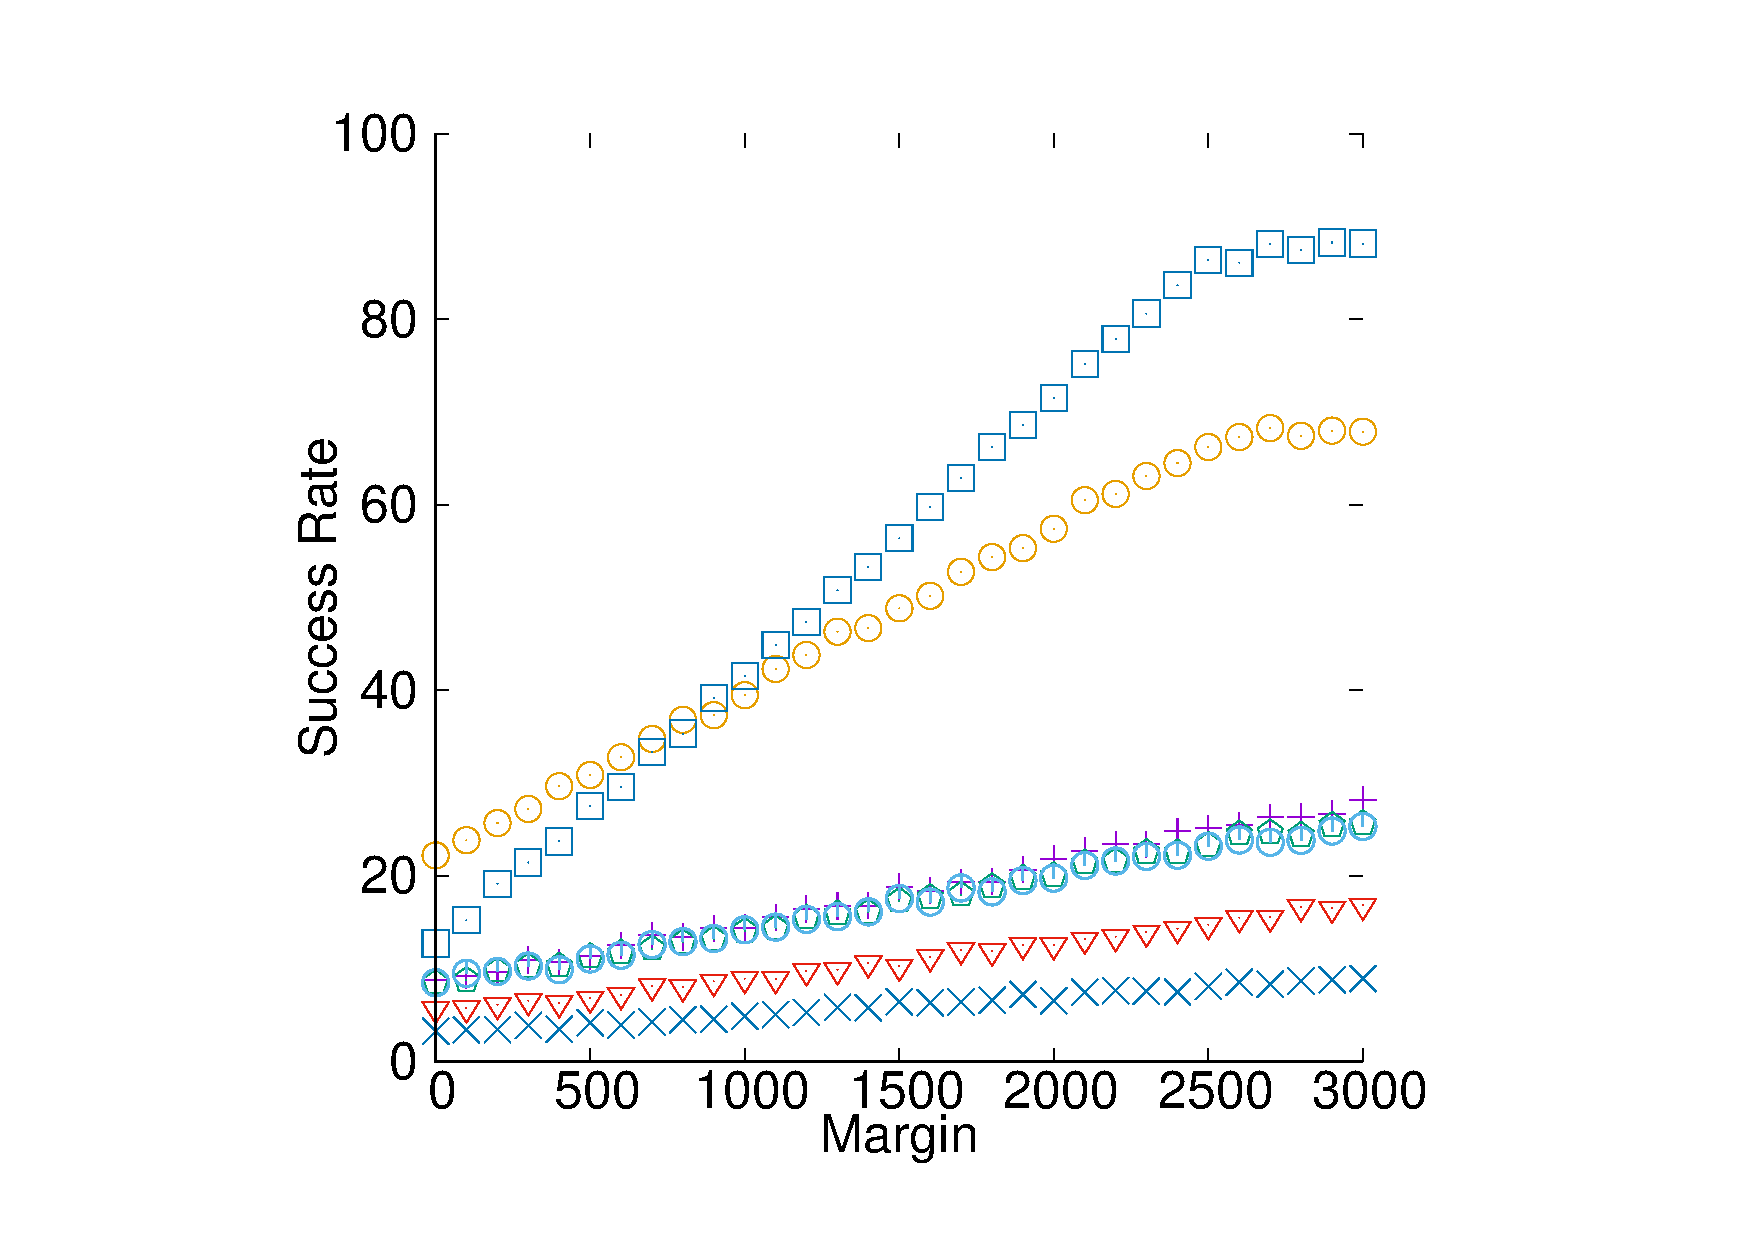
\includegraphics[height=5cm]{departs_gp_250001.pdf}
  \end{minipage}
  \begin{minipage}[b]{0.54\linewidth}
  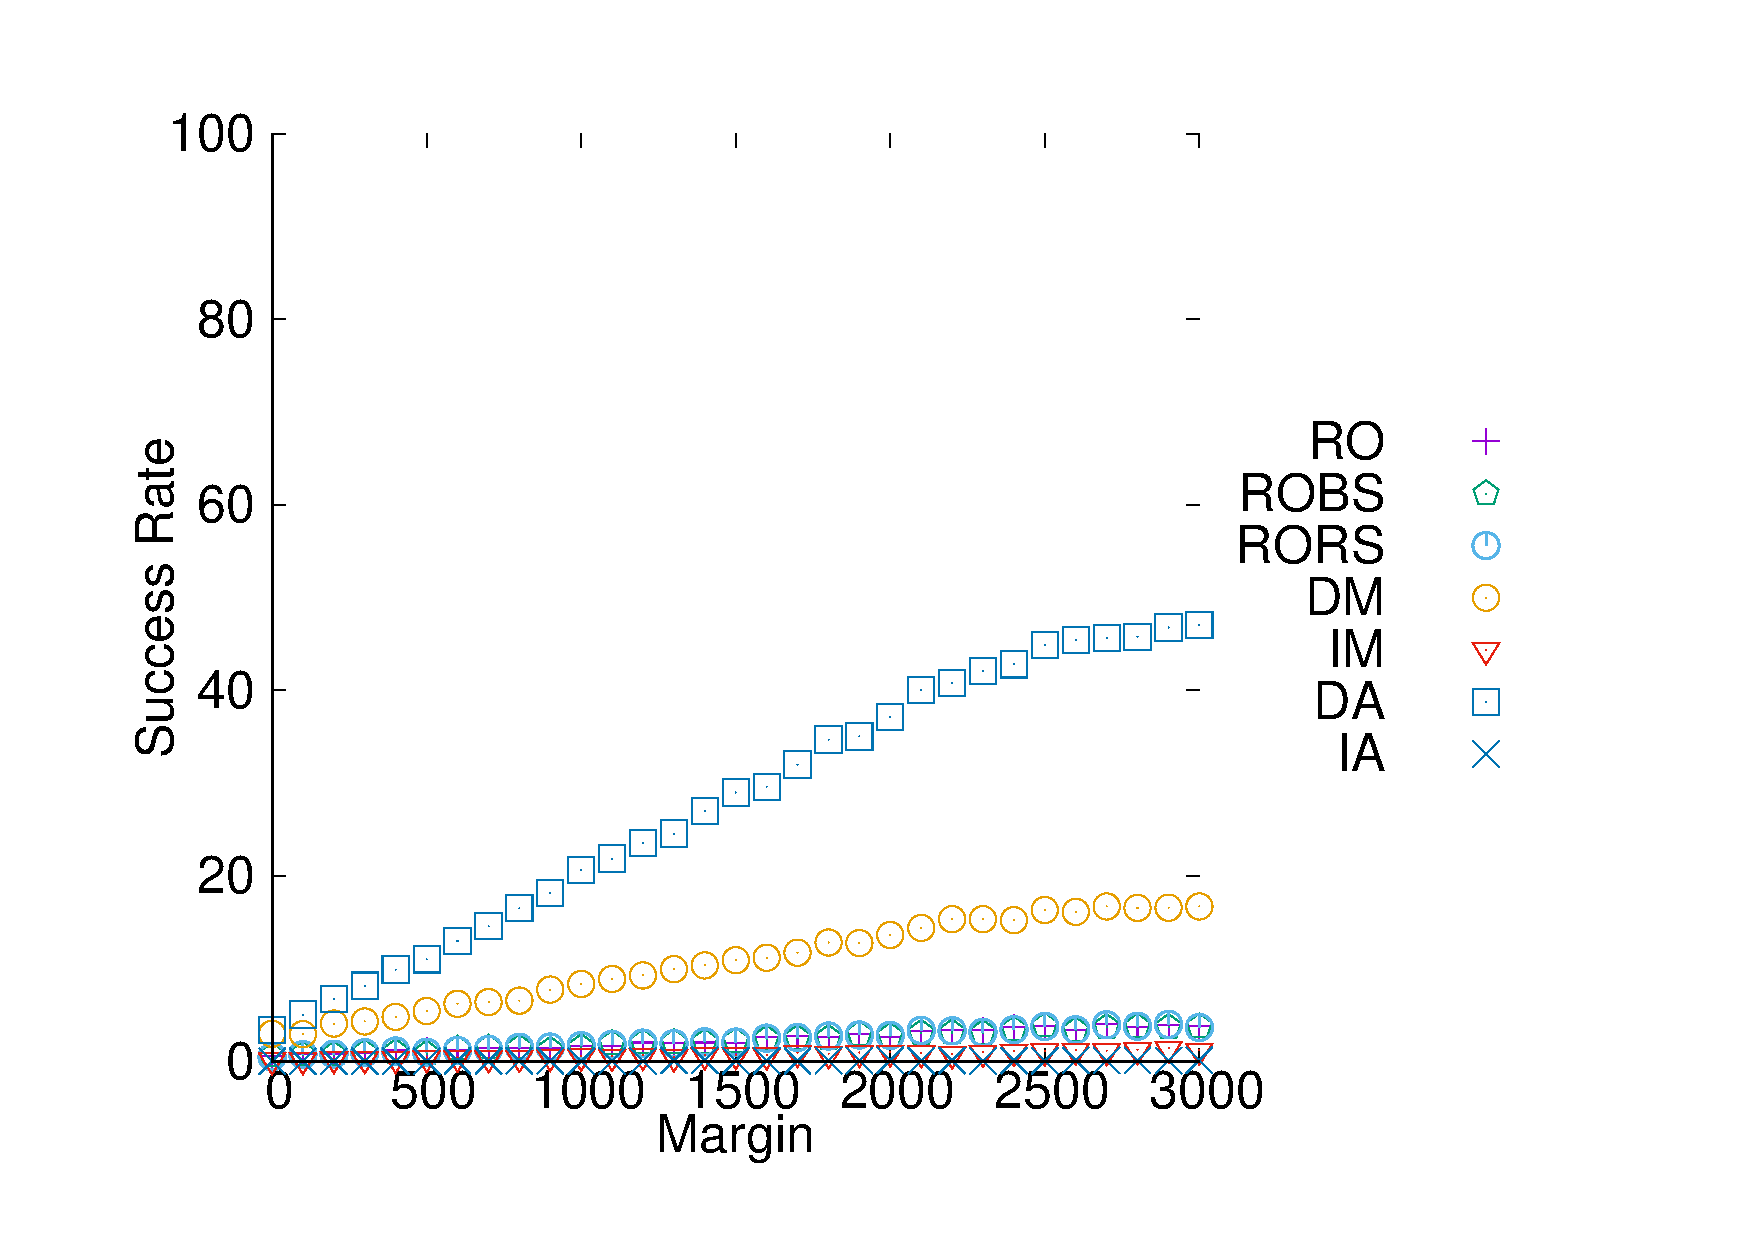
\includegraphics[height=5cm]{departs_gp_210001.pdf}

\end{minipage}
      \caption{Success rate of different sending orders, left $0.8$ load, right $0.95$ load.}
           \label{fig:success1random}
           \end{center}

     \end{figure}

          
     According to our experiments, policy IA, that is sending the datagrams on increasing order on the length of the arcs $(c_1,c_2)$, does not work well. It corresponds to the policy of Proposition~\ref{prop:SL} which we already know to be bad for \pazl when the routes are long as in this experiment. Sending in decreasing order on the margin of the routes (DM) or on the length of the arcs $(c_1,c_2)$ (DA) work better and it seems that DA is better than DM, especially in a loaded network. 
     
     Sending the datagrams using a random order does not perform well,
     but is still better than IM and IA, which shows that the latters are a poor choice for the first stage of our algorithm. The interest of using a random order is that we can draw many of them. In Figure~\ref{fig:success1000random}, the same experiment is made for the three random heuristics, but we now draw $1,000$ different random orders and solve each induced instance of \wta using \greedydeadline. The algorithm is considered to succeed as soon as a valid assignment is found for one order. Each random order drawn is used for RO, RORS and ROBS to make the comparison fairer.

\begin{figure}[h] 
  \centering
  \begin{minipage}[b]{0.45\linewidth}

  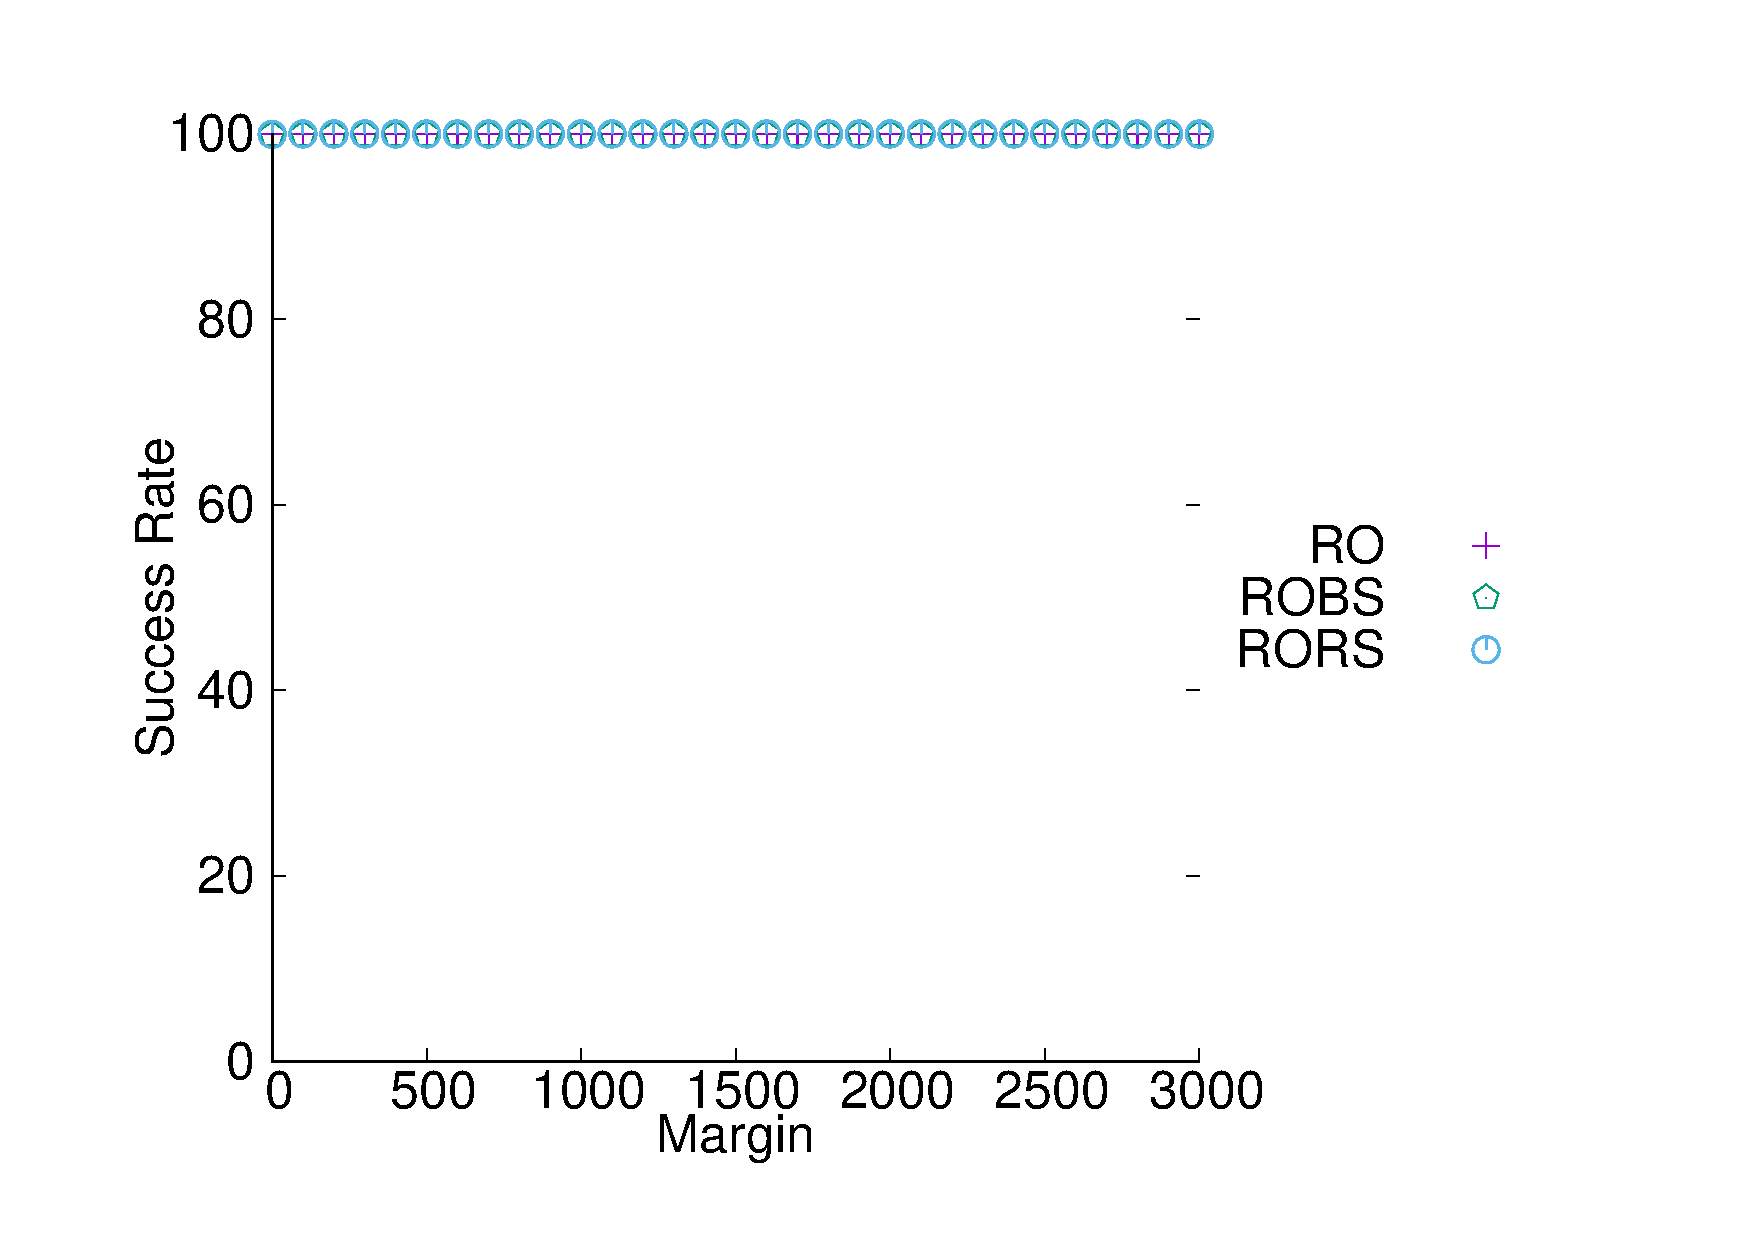
\includegraphics[height=5cm]{departs_gp_25000.pdf}
  \end{minipage}
  \begin{minipage}[b]{0.54\linewidth}
  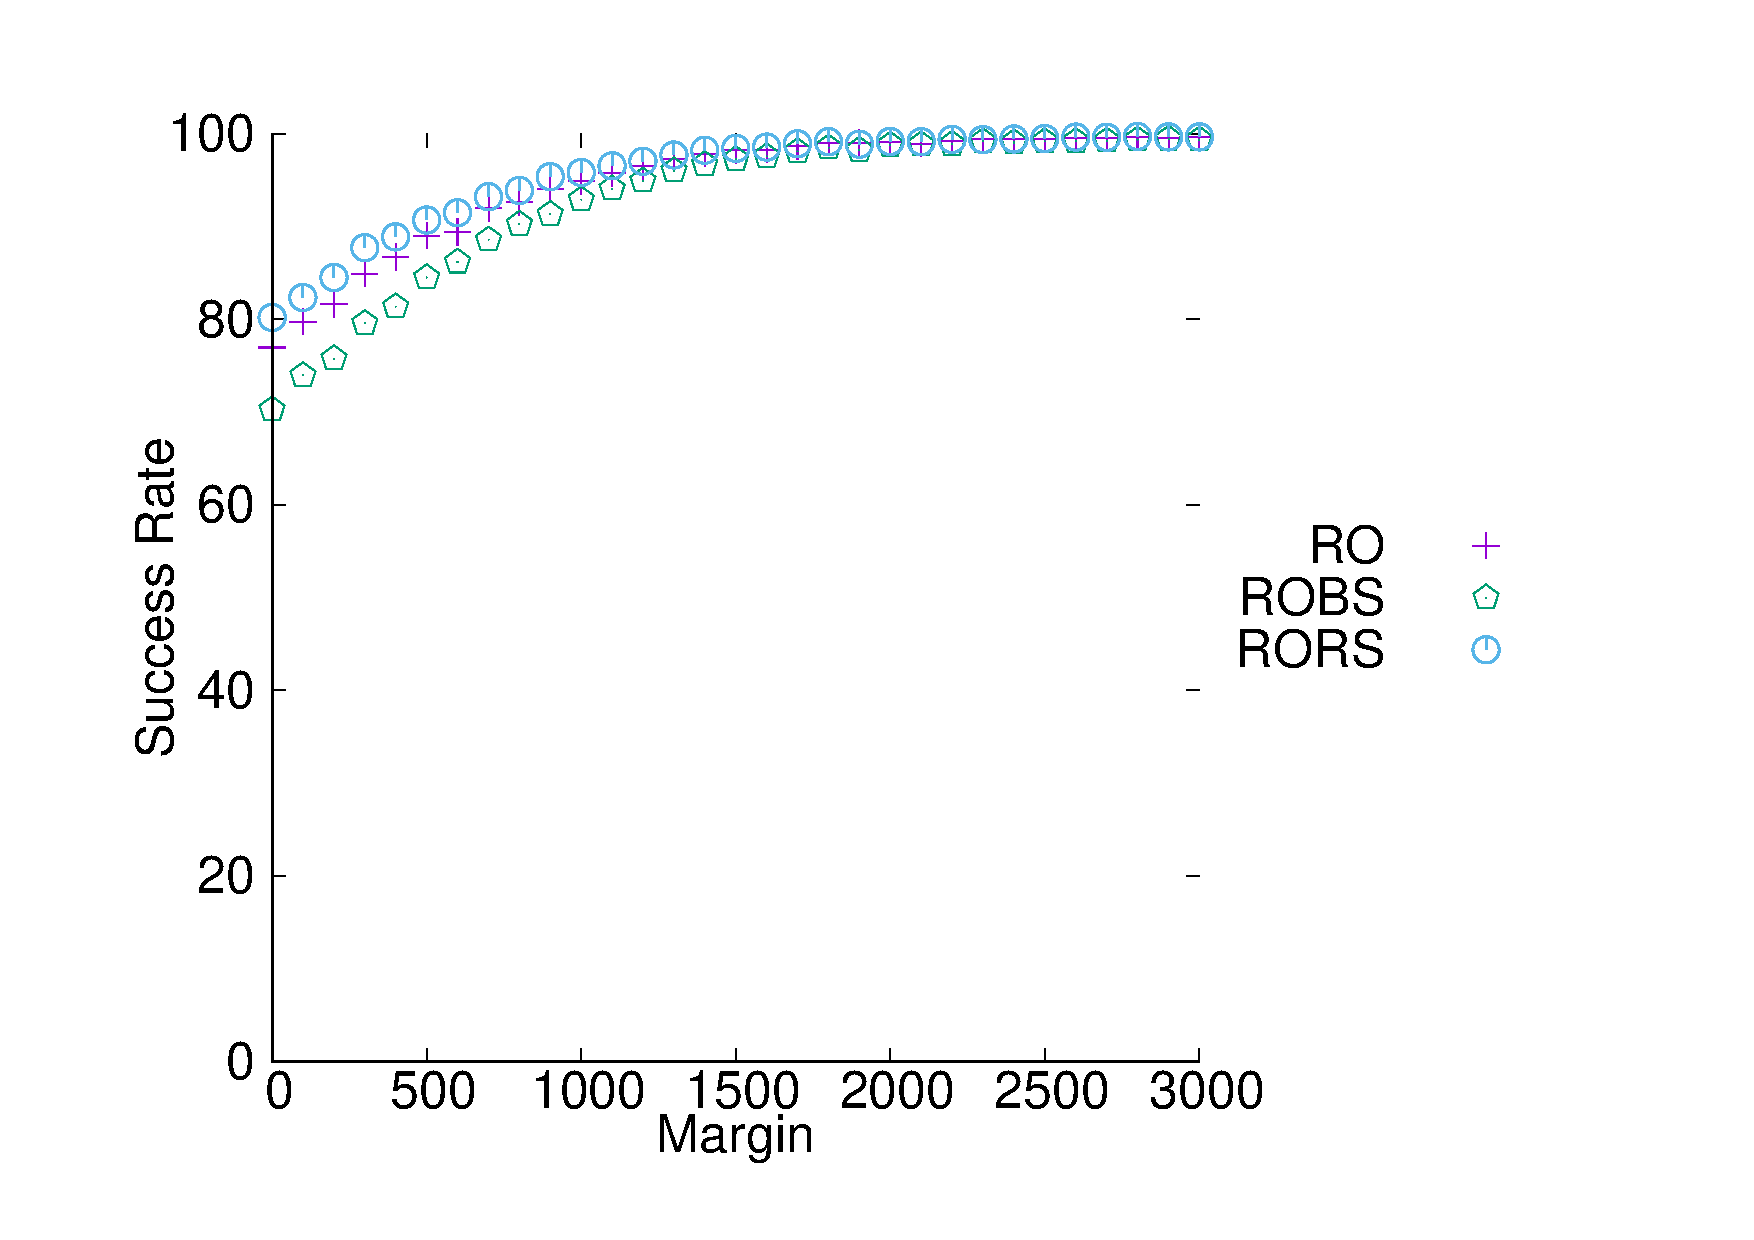
\includegraphics[height=5cm]{departs_gp_21000.pdf}

\end{minipage}
       \caption{Success rate of different sending orders with the random orders generated $1000$ times, left $0.8$ load, right $0.95$ load.}
      \label{fig:success1000random}
          \end{figure}

     Our algorithms find assignments with margin $0$ for many instances with $0.95$ of load and long routes which is not possible when only looking for bufferless assignments (see Section~\ref{sec:exp_PAZL}). It justifies the interest of studying \pall and not only \pazl.
  
     Using many random orders is much better than DA, the best policy using one specific order. 
     With a load of $0.95$, a solution is found with margin $0$ most of the time. The three random order policies have similar performances, but RORS has slightly better success rate than the two others ones, under high load and small margin. Hence, in the following experiments, we always draw $1,000$ random orders using the policy RORS to set the offsets of the assignments.
     

    \paragraph{Comparison of the algorithms solving \texttt{WTA}}

     We now compare the performances of the four different algorithms used in the second stage to set the waiting times. Since \greedydeadline already finds assignments with margin $0$ under a mild load of $0.8$, it is more interesting to focus on the behavior of the algorithms under a high load of $0.95$. In Figure~\ref{fig:success21000}, we represent the success rate of the four algorithms with regards to the margin, computed over $10,000$ random star routed networks generated with the same parameters as previously. 
     
    \begin{figure} [h] 
       \begin{center}
      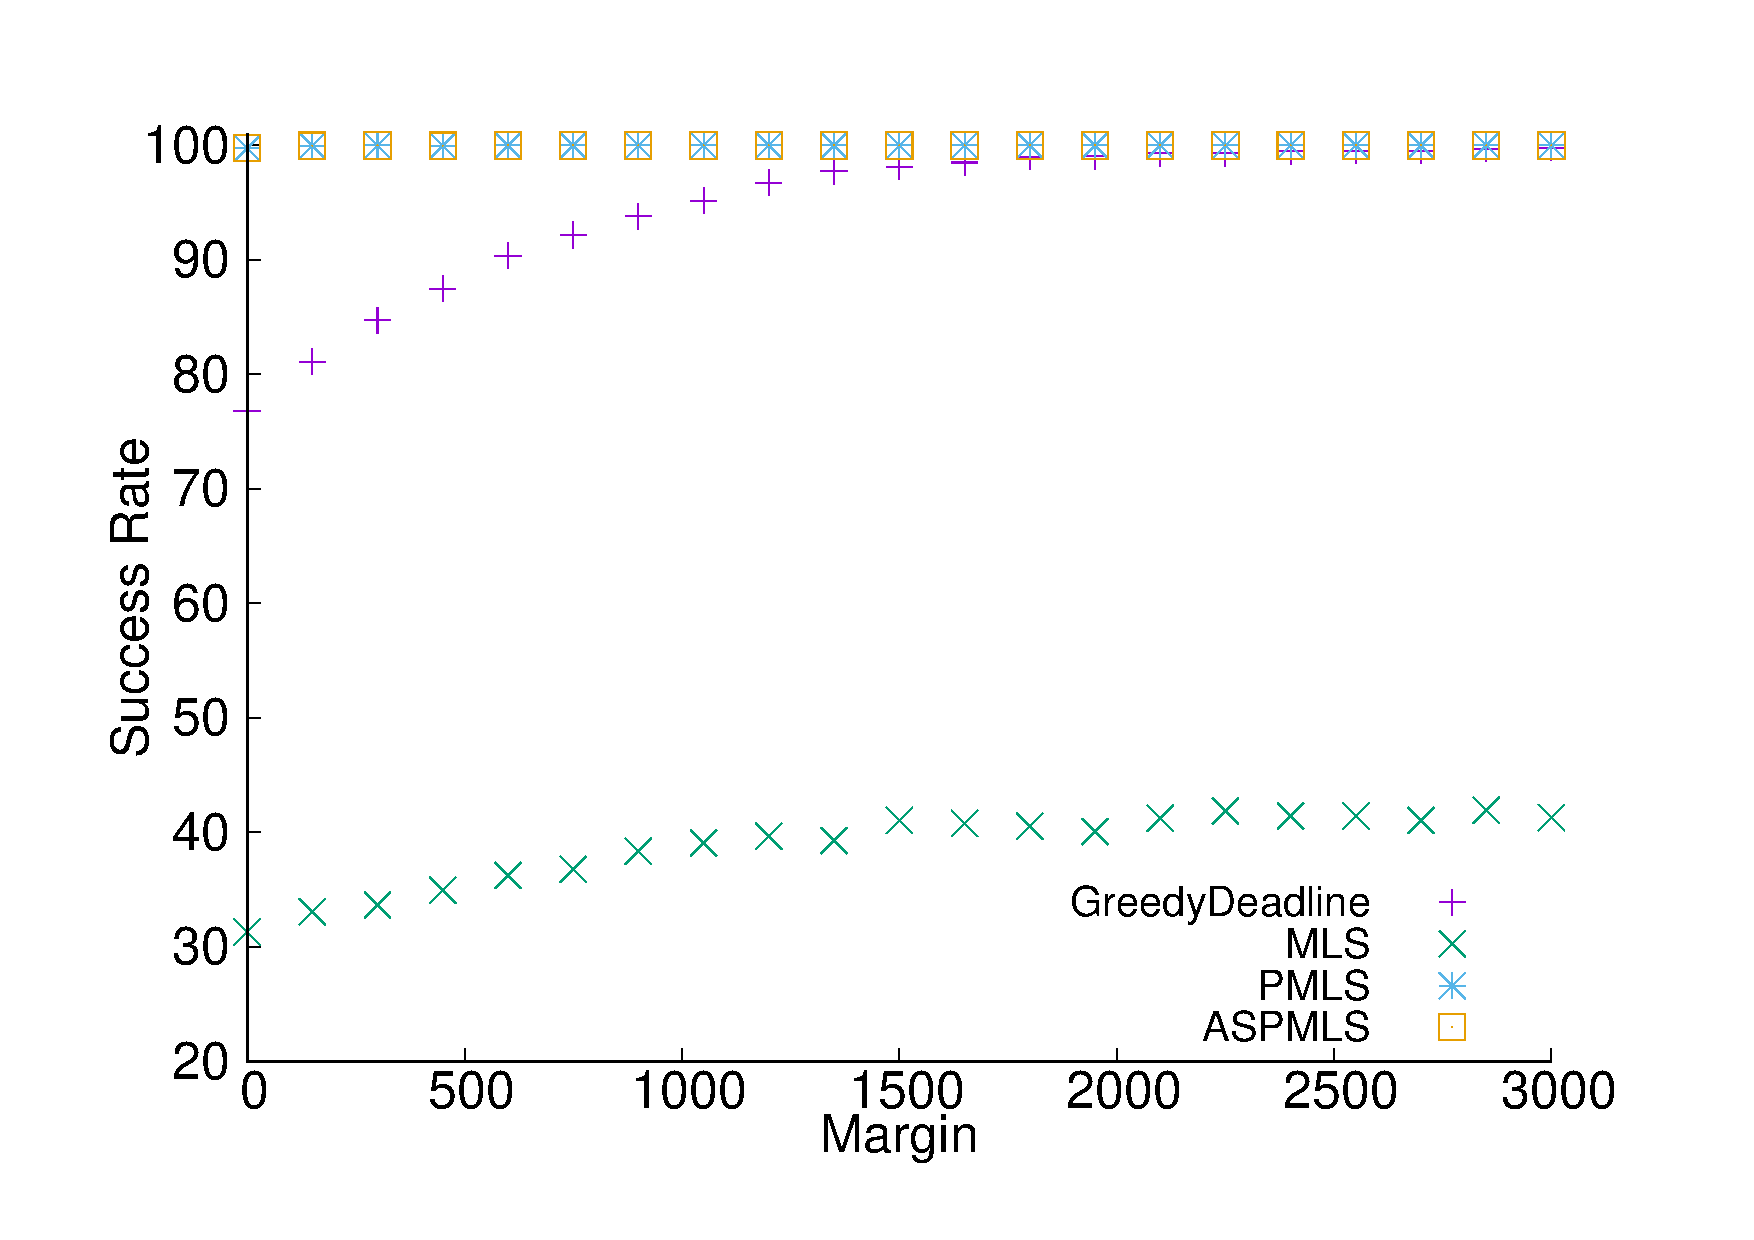
\includegraphics[width=0.8\textwidth]{retour_21000.pdf}
      \end{center}
      \caption{Success rate of four algorithms solving \pall, $0.95$ load}
     \label{fig:success21000}
     \end{figure}
     
      As explained in section~\ref{sec:wtaheuristic}, the \MLS algorithm does not consider periodicity while computing the waiting times, unlike the others algorithms for \wta. This explains why \MLS performs poorly, worst than \greedydeadline, \PMLS and \ASPMLS, and shows that \emph{taking into account the periodicity} is fundamental.
      \greedydeadline is close to $100\%$ success rate for margins larger than $1,500$ while  \PMLS and \ASPMLS algorithms find a solution for more than $99\%$ of the random instances, even \emph{with a margin $0$}. In other words, for very high load and no margin, there are very few instances for which we do not find an assignment. With a margin of $300$, which corresponds to about $15\mu$s of additional delay with the chosen parameters, we always find a solution. 
     
     It turns out that the performances of \PMLS and \ASPMLS are almost identical. Even with a load of $1$ and a margin of $0$, we have to draw $100,000$ random instances before finding one which can be solved by \ASPMLS and not by \PMLS. Since \ASPMLS is of exponential complexity in $n$, it may not be relevant to use it within the parameters of this experiment. To verify that, we present the computing time of \PMLS and \ASPMLS for different instance sizes. To stress the algorithms, we set the margin to $0$ and the load to $0.95$. The table of Figure~\ref{fig:tps_fpt} shows the computation times of \PMLS and \ASPMLS, averaged on $1,000$ instances. Recall that both \PMLS and \ASPMLS use the same first stage which produces $1000$ instances of \wta, using the policy RORS.

     
          \begin{figure}[h] 
       \begin{center}
   \begin{tabularx}{0.8\textwidth}{|c|X|X|X|X|X|X|}
    \hline
    \# routes& $8$ & $12$ & $16$& $20$ & $24$\\
    \hline
    \ASPMLS (ms) & $1.88$ &$5.98$&$47.75$&$209.2$&$1815$\\
    \hline
     \PMLS (ms) & $0.07$ &$0.08$&$0.09$&$0.10$&$0.12$\\
    \hline
    Ratio & $27$ &$78$&$523$&$2122$&$14882$\\
    \hline
      \end{tabularx}
      \end{center}
   \caption{Computation time for \PMLS and \ASPMLS function of the number of routes}
        \label{fig:tps_fpt}
     \end{figure}
    

  The complexity of both algorithms depends on the number of routes. As shown in Figure~\ref{fig:tps_fpt}, the time complexity of \PMLS seems linear on \emph{average}, while its theoretical worst case complexity is roughly quadratic. \ASPMLS scales exponentially with the number of routes as expected. Both algorithms are fast enough for instances of less than $20$ routes, but for $40$ routes or more \ASPMLS becomes too slow. Since \ASPMLS almost never finds a solution when \PMLS does not and is much slower, one should prefer to use \PMLS. 

    When evaluating the computing time of our method, we should take into account how many random orders are drawn. In previous experiments, we have drawn $1,000$ random orders which may be $1,000$ time slower than using a single fixed order. There is a trade-off between the number of random orders and the success rate. We investigate the success rate of our algorithms with regards to the number of random orders drawn, a load of $0.95$ and a margin $0$. The table of Figure~\ref{fig:randomdrawing} presents the success rate for different numbers of sending orders, averaged over $10,000$ instances, for \greedydeadline, \PMLS and \ASPMLS.


         \begin{figure}[h] 
       \begin{center}
   \begin{tabularx}{0.8\textwidth}{|c|X|X|X|X|X|X|}
    \hline
    \# orders& $1$ & $10$ & $100$& $1,000$& $10^{4}$&$10^{5}$\\
    \hline
    \greedydeadline & $0.55$ &$6.05$&$35.44$&$77.43$&$90.1$&$92.4$\\
    \hline
    \PMLS & $82.04$ &$98.84$&$99.71$&$99.80$&$99.83$&$99.83$\\
    \hline
    \ASPMLS & $91.33$&$99.17$&$99.72$&$99.80$ &$99.83$&$99.83$\\
    \hline
      \end{tabularx}
      \end{center}
   \caption{Success rates function of the number of random orders drawn in the first stage of the three algorithms}
        \label{fig:randomdrawing}
     \end{figure}

	First, observe that the better the algorithm to solve $\wta$ is, the fewer random orders it needs in stage one to achieve its best success rate. In particular, \ASPMLS has better results than \PMLS for less than $1,000$ random orders, but not beyond. This further justifies our choice to draw $1,000$ random orders, to obtain the best success rate within the smallest time.

	The number of different orders is $7!= 5,040$ since we have $8$ routes and the solutions are invariant up to a circular permutation of the order. Hence, for $8$ routes it is possible to test every possible order. However, the computation time of this exhaustive method scales badly with $n$. The fact that \PMLS and \ASPMLS have already high success rates for $10$ random orders hints that even for a larger number of routes, drawing $1000$ random orders is sufficient to obtain good assignments.


     \paragraph{Harder Topologies}
     
    Previous experiments use instances with weights of arcs uniformly drawn in a large interval. However, it is quite natural to consider that most routes are of roughly the same length or can be arranged in two groups of similar length, when the fronthaul network involves one or two data centers.
    
		  By Proposition~\ref{prop:asym}, there is an assignment with margin equal to the maximum difference
    between the sizes of the routes. Hence, if all routes have almost the same size, the needed margin is small. If the routes are drawn uniformly in a large interval, then the expected difference between the longest route and the second longest route is large. This difference can be seen as a free waiting time for most routes, hence we expect to need little margin in this regime too. As a consequence, the harder instances should be for routes with length drawn in an interval of moderate size compared to the period.

  	Figure \ref{fig:2grp} shows the probability of success of \PMLS  over $10,000$ instances as a function of the margin. In the left experiment, the weights of the arcs are drawn in $[0,I]$, where $I$ goes from $0$ to $6400$. As expected the success rate decreases when the size of the interval increases, until $I = 1600$, and then increases again.  In the most difficult settings, only $78\%$ of the instances can be solved with margin $0$, and we need a margin of $1,900$ to ensure that \PMLS always finds a solution. Results for \ASPMLS are not shown, since they are the same as for \PMLS, even on these hard instances.

 	 We do the same experiment at the right of the figure, except that the weights of arcs of half of the routes are drawn in $[I]$ and the weights of the other half are drawn in $[P/2,P/2 + I[$. The situation is the same as for the previous experiment but with better success rates, hence the case of two data centers seems simpler to deal with.
  
           \begin{figure}
        %   \begin{minipage}{0.49\linewidth}
    
       \begin{center}
      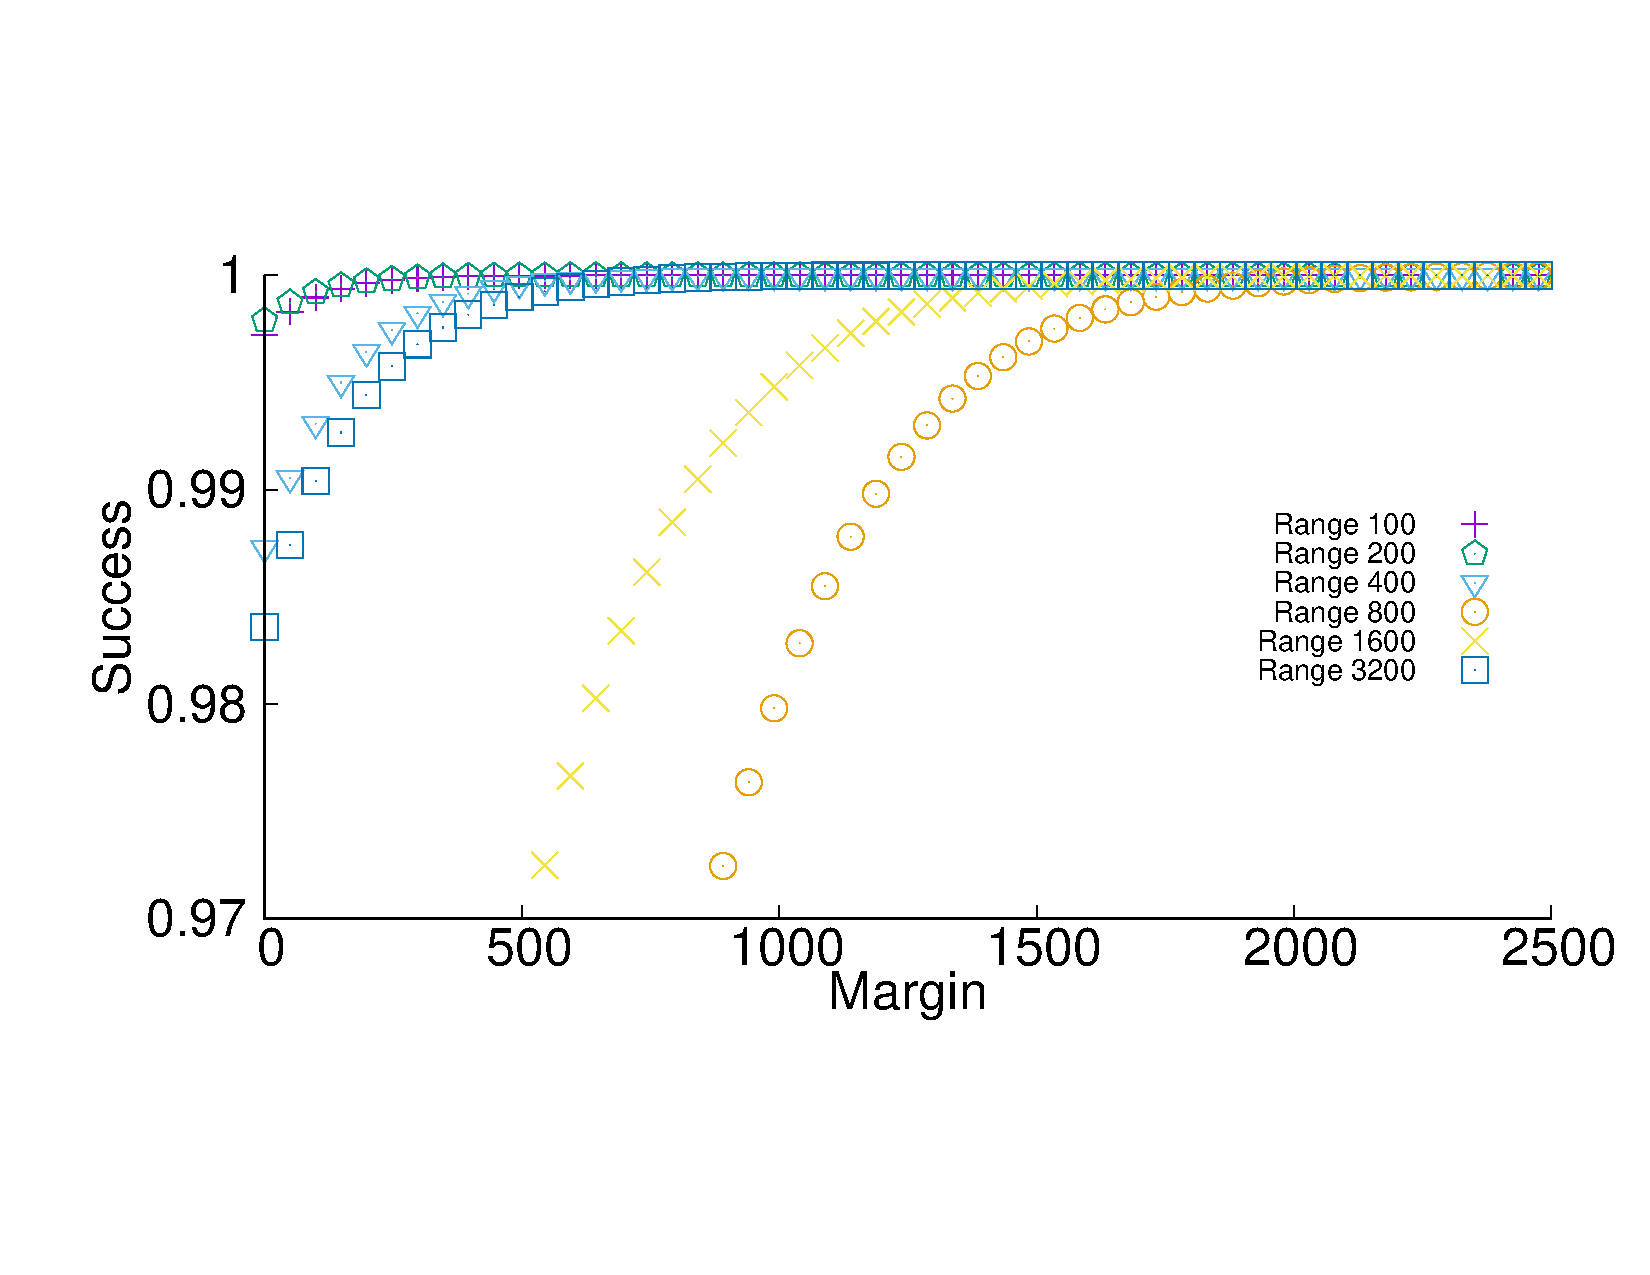
\includegraphics[width = 0.9\linewidth]{departs_distrib1Grp.pdf}
     
     
     
 %\end{center}
   %\end{minipage}\hfill
%\begin{minipage}{0.48\linewidth}   
         
      % \begin{center}
      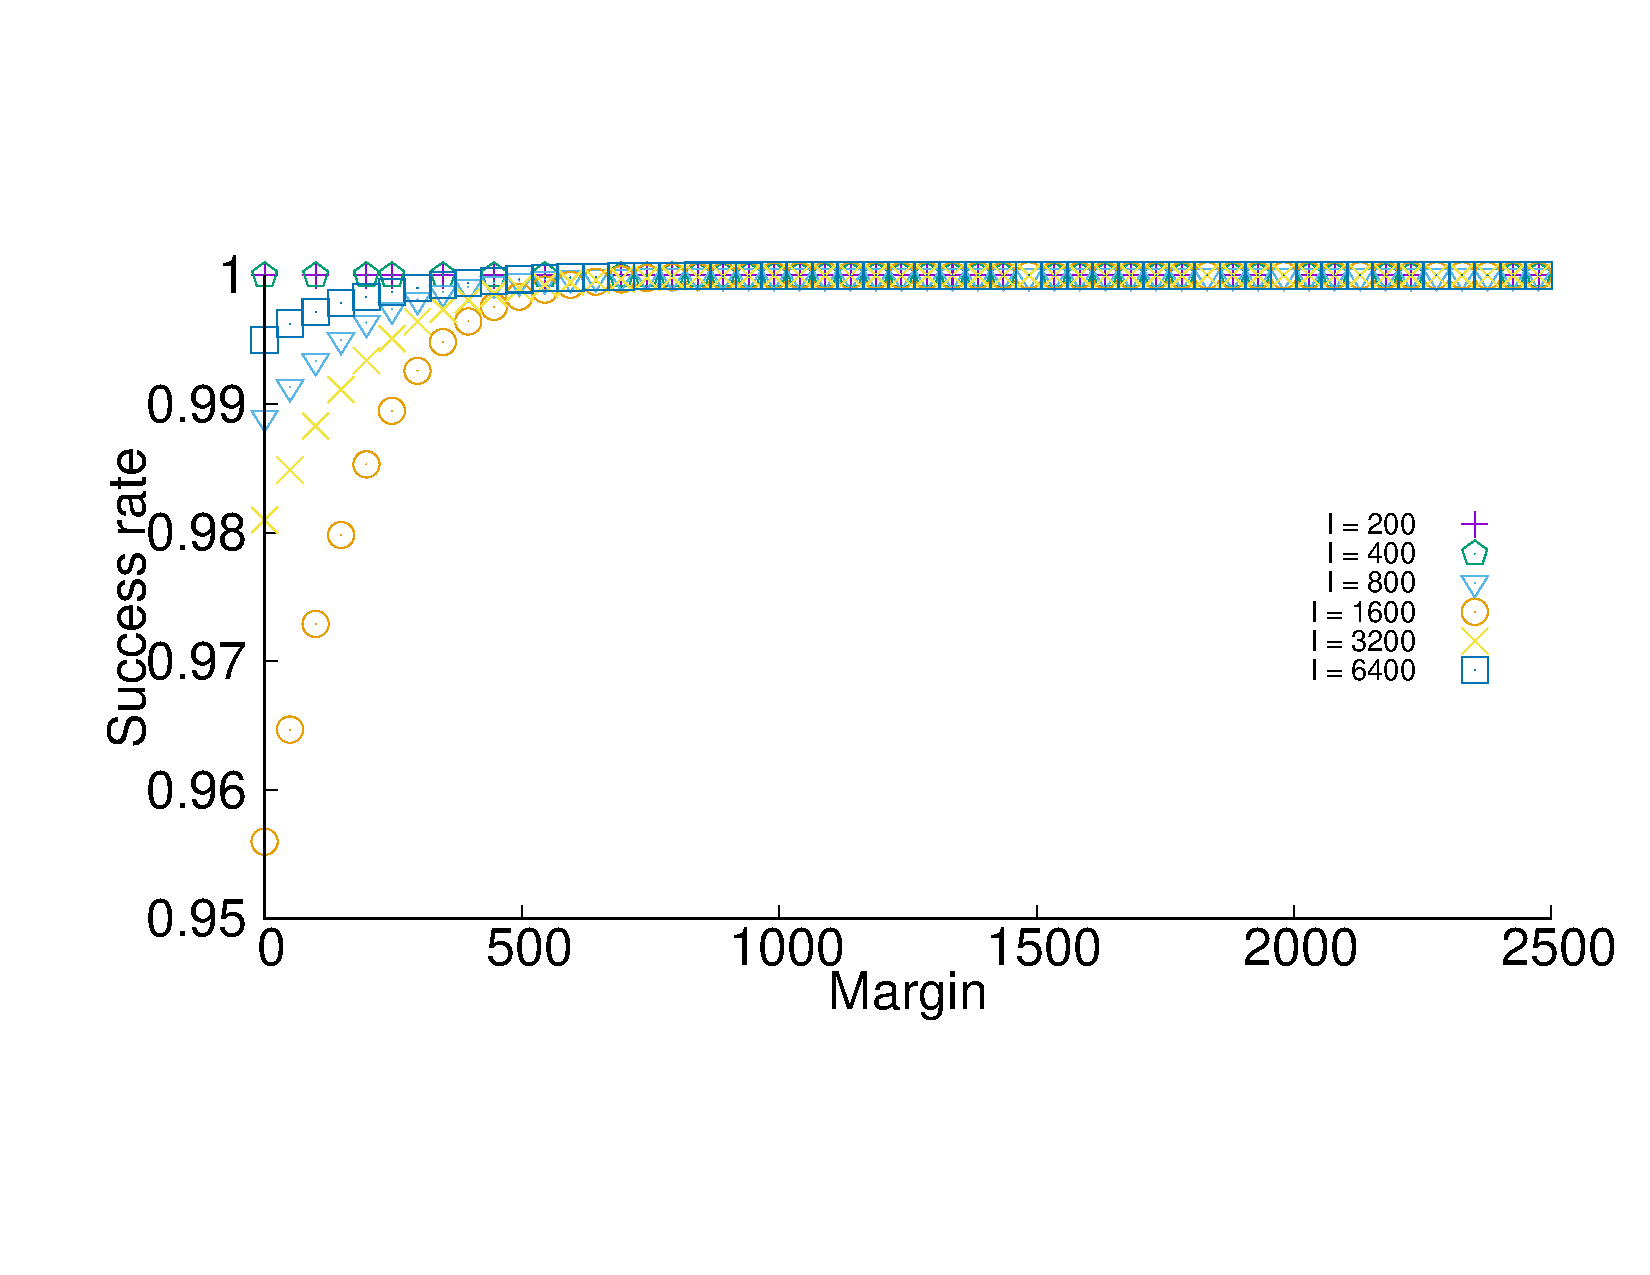
\includegraphics[width = 0.9\linewidth]{departs_distrib2Grp.pdf}
   
  
         \end{center}
      %\end{minipage}\hfill
         \caption{Success rate of \PMLS, with length of arcs drawn either in $[I]$ (top) or in $[I]$ or $[P/2,P/2 + I[$ (bottom).}
      \label{fig:2grp} 
  \end{figure}
\section{Deterministic Assignments vs Statistical Multiplexing}\label{sec:comparison}

    \subsection{Performance of Statistical Multiplexing}


  %    \subsubsection{Description of statistical multiplexing}
      Now that we have designed and tuned \PMLS to solve \pall efficiently, we compare its performances against the actual way to manage the messages in a network:  \emph{statistical multiplexing}, with a \FIFO buffer in each node of the network to resolve collisions. For statistical multiplexing, the time at which the datagrams are sent in the network is not managed by the user as in our approach, thus we assume the offset of each route is fixed to some random value, and stays the same over time.
      We consider a second policy to manage buffers called \critdead. In a buffer with several datagrams, this policy sends the one with the smallest remaining margin, which is the time it can wait before missing its deadline.


    We have implemented a statistical multiplexing simulator, to evaluate the performance of these two policies. We compare them to our solution, finding an assignment with the smallest possible margin using \PMLS. 
    For statistical multiplexing, both contention points have a buffer. The process is not periodic:
    even if the offset of a route is the same each period, it is possible that some datagram does not arrive at the same time in a contention point in two consecutive periods because of buffering. Therefore, we must measure the process time of each route over several periods if we want to compute the maximum latency of the network. We choose to simulate it for $1,000$ periods but we have observed that the process time usually stabilizes in less than $10$ periods. The \textbf{margin}, for statistical multiplexing, is defined as the maximum process time, computed as explained, minus the size of the longest route of the star routed network. 

%In the network we study here, two kinds of traffic are present: the Cloud Ran traffic, the one we studied in this paper, and another traffic, less critical, for which there is no needed guarantee, the Best Effort (BE) traffic. We propose three policies to manage the traffics in the nodes.

      %Even if this policy seems to work in practice when the network is not too loaded, it does not give any guarantee on the latency. 

     In Figure~\ref{fig:sto}, we represent the probability of success of statistical multiplexing and \PMLS for different margins. The success rates are computed from $10,000$ star routed networks for each margin. On the top of Figure~\ref{fig:sto}, the arcs of the network are uniformly drawn in $[P]$, while on the bottom of Figure~\ref{fig:sto}, the arcs of the network are uniformly drawn in $[1600]$ (the hardest settings of the previous section). The other parameters of the experiences are the same as previously and the load is $0.95$. 
     
    \begin{figure}


%\begin{minipage}{0.49\linewidth}
       \begin{center}
      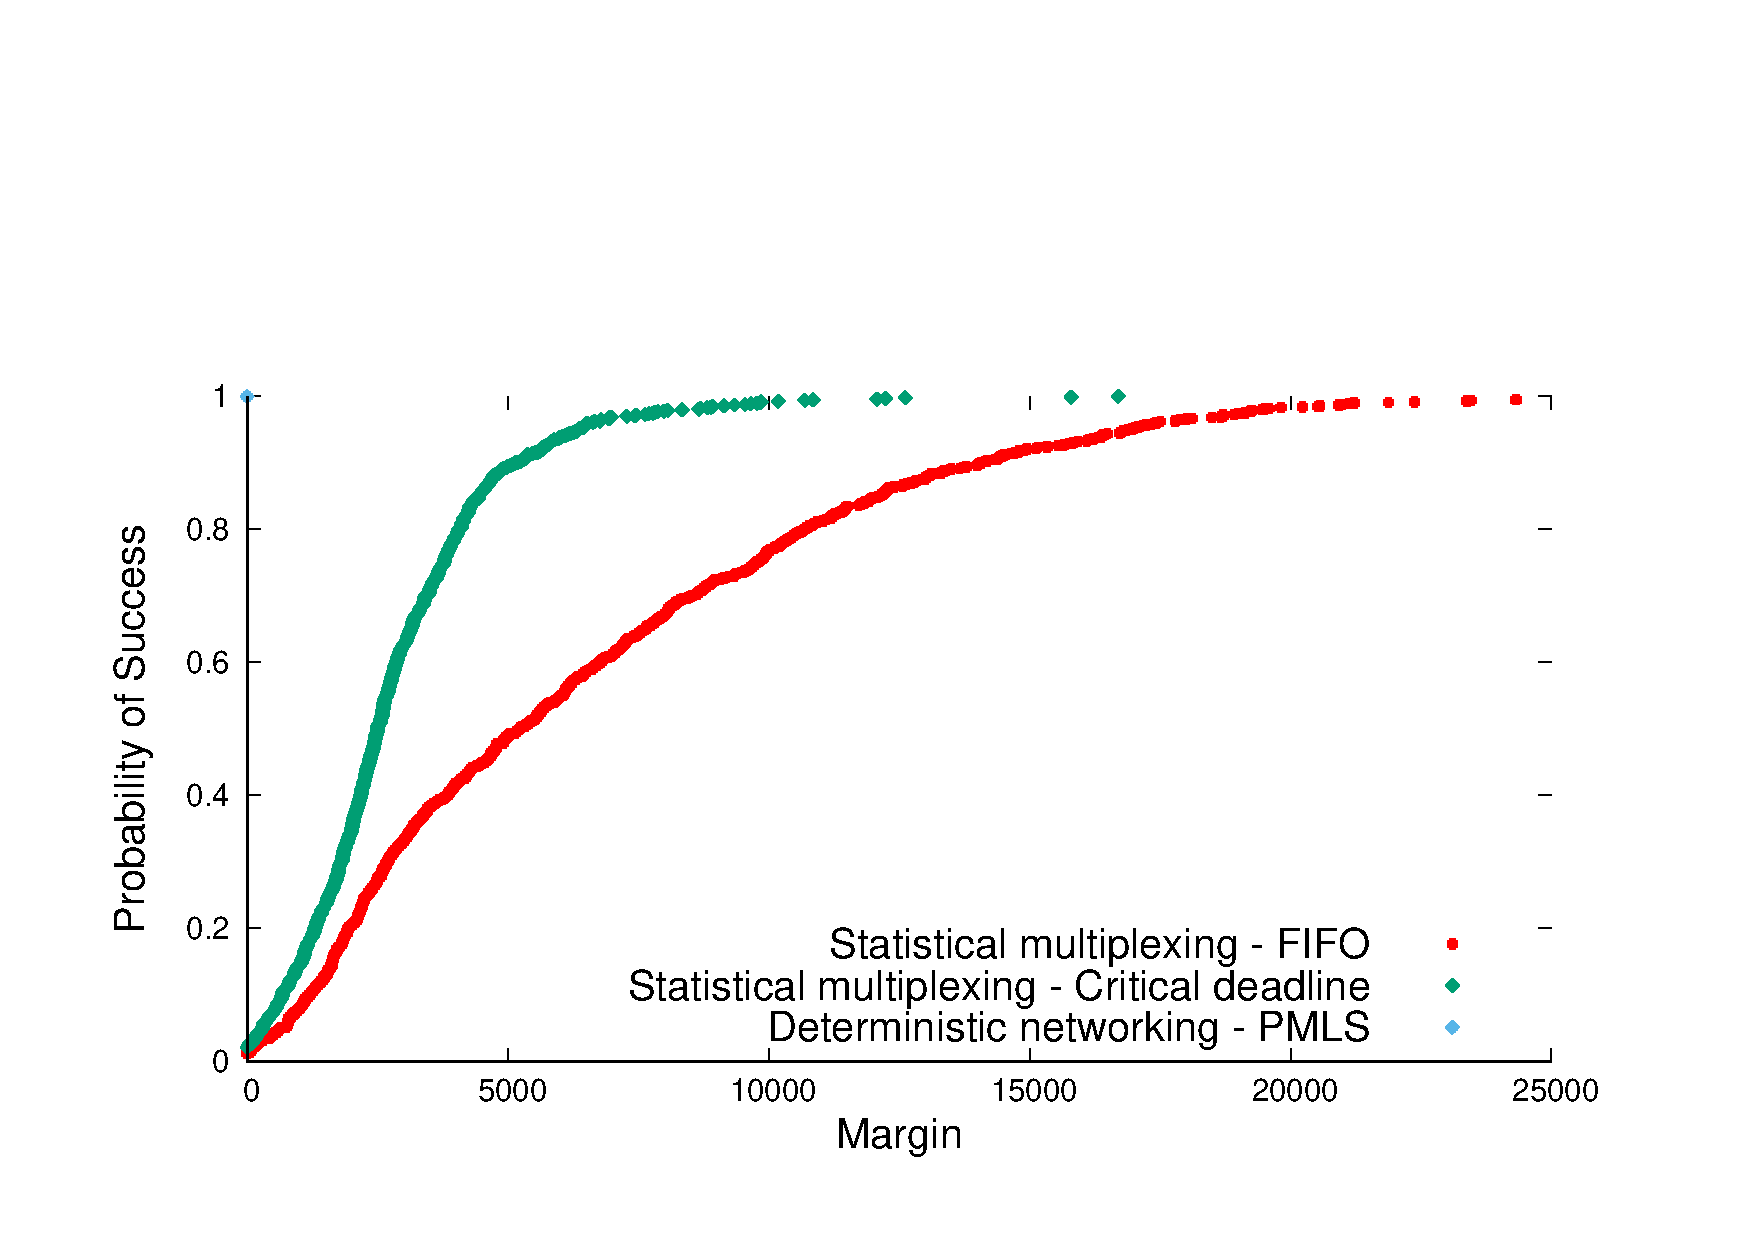
\includegraphics[width = 0.9\linewidth]{stochasticdistrib.pdf}
     % \end{center}
   %\end{minipage}\hfill
%\begin{minipage}{0.49\linewidth}   

     %  \begin{center}
     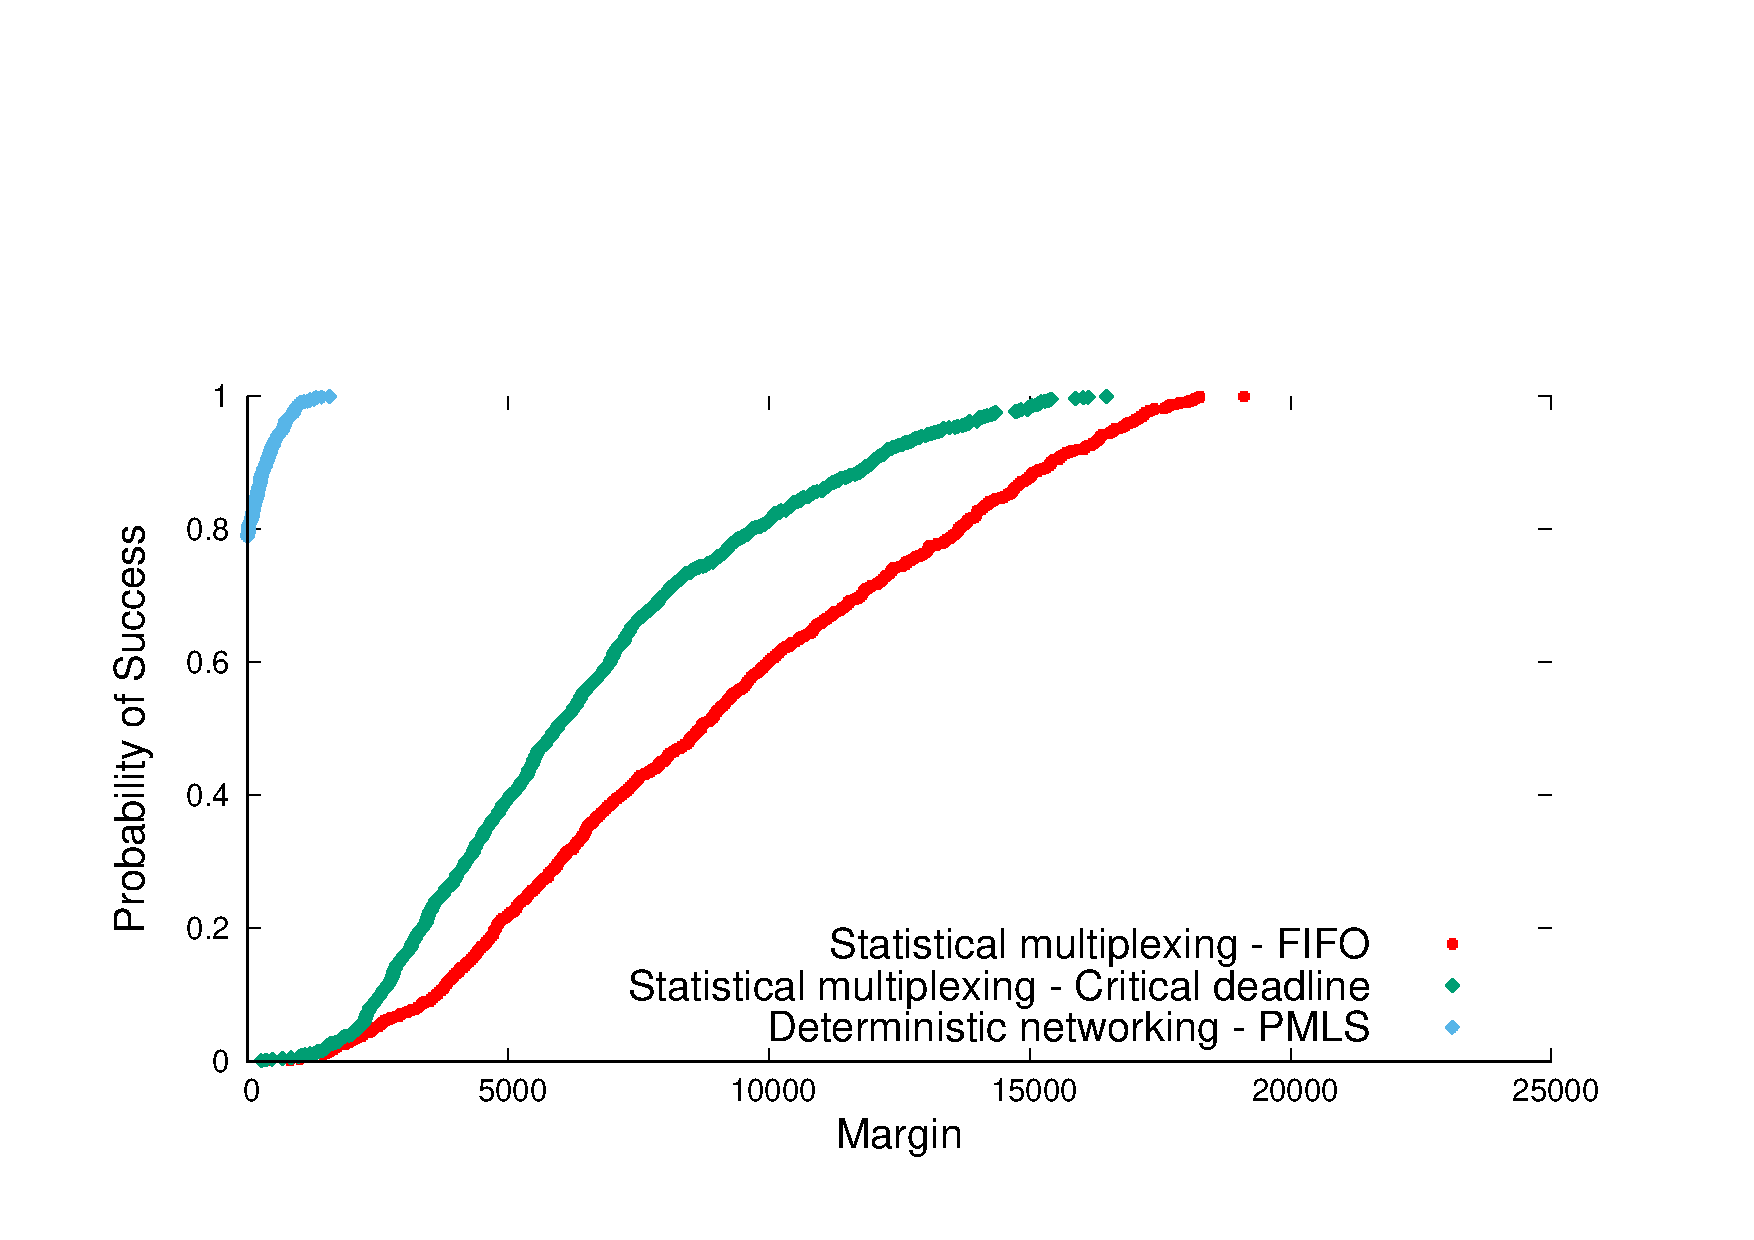
\includegraphics[width = 0.9\linewidth]{stochastic.pdf}

       \end{center}
    %  \end{minipage}\hfill
      
      
  \caption{Probability of success of statistical multiplexing and \PMLS for several margins on random topologies when the size of the routes are distributed either on $P$ (top) or on a small range of values (bottom).}
      \label{fig:sto} 
      \end{figure}

   The experiment shows that statistical multiplexing cannot ensure a small enough latency. 
    For random topologies, the latency is extremely high when using FIFO ($6538$ tics on average), with a margin of about $10,000$ for the worst $30\%$ of instances, which corresponds to half the period ($0.5$ms). Even when the messages are managed with \critdead, $20\%$ of the instances have a margin of more than $4,000$ ($2838$ tics on average) while PMLS finds an assignment with $0$ margin $99\%$ of the time! 
    
    For hard topologies (right figure), the average margin of statistical multiplexing ($9052$ tics for FIFO, $6574$ tics for \critdead) is worst than for random topologies. The worst case of \critdead  remains the same ($\simeq 16500$ tics) while the worst case of FIFO fall from $30828$ tics for random topologies to $19105$ tics on hard topologies. The settings are stressful for \PMLS, and we find an assignment with margin $0$ in only $78\%$ of the instances, and it needs a margin of $2,000$ tics to be sure to find an assignment. However, \PMLS still vastly outperforms the statistical multiplexing both for the average margin and for the worst margin. 
    
    Even under a light load of $0.4$, for which we can always find bufferless assignment, statistical multiplexing has a very high average margin ($1290$ tics for FIFO and $1052$ tics for \critdead) and worst case margin ($10963$ tics for FIFO and $6938$ tics for \critdead).

    For each $1,000$ tics of latency we save from the periodic process, we are able to lengthen the routes by $10$km, which has a huge economical impact. We feel that it strongly justifies the use of a deterministic sending scheme for latency-critical applications such as our C-RAN motivating problem.    
     
    \subsection{Periodic Assignment and Random Traffic}
    
    The algorithms proposed in this paper are designed to manage deterministic periodic flows in dedicated networks. In this section, the objective is to determine the effect of adding in the network non-deterministic flows (internet traffic, best-effort) managed by statistical multiplexing.

    The algorithms solving \pall are not designed to take into account additional best-effort traffic. In particular, they often build very compact assignments, with all datagrams following one another in a contention vertex, which is bad for the latency of best-efforts datagrams trying to go through the same contention point. Thus, we propose an adaptation of any algorithm solving \pall, to find assignments where the unused tics are as evenly spaced as possible in the period. Such assignments minimize the maximal latency of any random datagram trying to go through the contention points. A similar approach, to decrease the latency of best-effort datagrams while scheduling C-RAN datagrams on an optical ring, can be found in~\cite{DBLP:conf/ondm/BarthGS19}.
    
    
    \subsubsection{Spaced Assignments}

    Most algorithms for \pall, when determining the waiting times, send datagrams as early as possible
    and thus create long sequences of datagrams in $c_2$, without free tics between them. We propose to modify any algorithm solving \pall on an instance with datagram size $\tau$ as follows: compute a $(P,\tau')$ assignment using the algorithm, for the largest possible $\tau' \geq \tau$. 

    \begin{lemma}\label{lemma:smaller_tau}
    Let $I' = (N,P,\tau',d)$ be an instance of \pall, for which there is an assignment, and let 
    $\tau \leq \tau'$, then there is also an assignment for $I = (N,P,\tau,d)$.
    \end{lemma}  
    \begin{proof}
    Let $A$ be the assignment of $I'$, the absence of collision is the absence of 
    intersection between intervals $[r_i,c_1]_{P,\tau'}$ (and $[r_i,c_2]_{P,\tau'}$). 
    If we consider $A$ as an assignment of $I$, then the intervals of used tics are $[r_i,c_1]_{P,\tau}$ (resp. $[r_i,c_2]_{P,\tau}$). 
    These intervals are strictly included in $[r_i,c_1]_{P,\tau'}$ (resp. $[r_i,c_2]_{P,\tau'}$), hence they do not have intersection either. 
    \end{proof}


     Lemma~\ref{lemma:smaller_tau} gives a way to obtain a solution of an instance from the same instance with a larger message size, as illustrated in Figure~\ref{fig:space}. 
     This transformation guarantees that all datagrams are separated by at least $\tau' - \tau$ free tics in each contention point. We are interested in finding the maximal $\tau'$
    for which there is an assignment. Since the property of having an assignment is monotonous with regards to $\tau'$, we can do so by a dichotomous search on $\tau$.

           \begin{figure}
       \begin{center}
      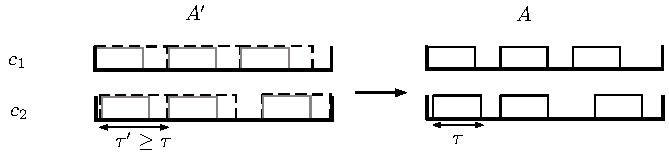
\includegraphics[width = 0.8\textwidth]{space.pdf}
       %% GNUPLOT: LaTeX picture
\setlength{\unitlength}{0.240900pt}
\ifx\plotpoint\undefined\newsavebox{\plotpoint}\fi
\sbox{\plotpoint}{\rule[-0.200pt]{0.400pt}{0.400pt}}%
\begin{picture}(1500,900)(0,0)
\sbox{\plotpoint}{\rule[-0.200pt]{0.400pt}{0.400pt}}%
\put(171.0,131.0){\rule[-0.200pt]{4.818pt}{0.400pt}}
\put(151,131){\makebox(0,0)[r]{$0$}}
\put(1279.0,131.0){\rule[-0.200pt]{4.818pt}{0.400pt}}
\put(171.0,212.0){\rule[-0.200pt]{4.818pt}{0.400pt}}
\put(151,212){\makebox(0,0)[r]{$1000$}}
\put(1279.0,212.0){\rule[-0.200pt]{4.818pt}{0.400pt}}
\put(171.0,293.0){\rule[-0.200pt]{4.818pt}{0.400pt}}
\put(151,293){\makebox(0,0)[r]{$2000$}}
\put(1279.0,293.0){\rule[-0.200pt]{4.818pt}{0.400pt}}
\put(171.0,374.0){\rule[-0.200pt]{4.818pt}{0.400pt}}
\put(151,374){\makebox(0,0)[r]{$3000$}}
\put(1279.0,374.0){\rule[-0.200pt]{4.818pt}{0.400pt}}
\put(171.0,455.0){\rule[-0.200pt]{4.818pt}{0.400pt}}
\put(151,455){\makebox(0,0)[r]{$4000$}}
\put(1279.0,455.0){\rule[-0.200pt]{4.818pt}{0.400pt}}
\put(171.0,535.0){\rule[-0.200pt]{4.818pt}{0.400pt}}
\put(151,535){\makebox(0,0)[r]{$5000$}}
\put(1279.0,535.0){\rule[-0.200pt]{4.818pt}{0.400pt}}
\put(171.0,616.0){\rule[-0.200pt]{4.818pt}{0.400pt}}
\put(151,616){\makebox(0,0)[r]{$6000$}}
\put(1279.0,616.0){\rule[-0.200pt]{4.818pt}{0.400pt}}
\put(171.0,697.0){\rule[-0.200pt]{4.818pt}{0.400pt}}
\put(151,697){\makebox(0,0)[r]{$7000$}}
\put(1279.0,697.0){\rule[-0.200pt]{4.818pt}{0.400pt}}
\put(171.0,778.0){\rule[-0.200pt]{4.818pt}{0.400pt}}
\put(151,778){\makebox(0,0)[r]{$8000$}}
\put(1279.0,778.0){\rule[-0.200pt]{4.818pt}{0.400pt}}
\put(171.0,859.0){\rule[-0.200pt]{4.818pt}{0.400pt}}
\put(151,859){\makebox(0,0)[r]{$9000$}}
\put(1279.0,859.0){\rule[-0.200pt]{4.818pt}{0.400pt}}
\put(171.0,131.0){\rule[-0.200pt]{0.400pt}{4.818pt}}
\put(171,90){\makebox(0,0){$20000$}}
\put(171.0,839.0){\rule[-0.200pt]{0.400pt}{4.818pt}}
\put(359.0,131.0){\rule[-0.200pt]{0.400pt}{4.818pt}}
\put(359,90){\makebox(0,0){$25000$}}
\put(359.0,839.0){\rule[-0.200pt]{0.400pt}{4.818pt}}
\put(547.0,131.0){\rule[-0.200pt]{0.400pt}{4.818pt}}
\put(547,90){\makebox(0,0){$30000$}}
\put(547.0,839.0){\rule[-0.200pt]{0.400pt}{4.818pt}}
\put(735.0,131.0){\rule[-0.200pt]{0.400pt}{4.818pt}}
\put(735,90){\makebox(0,0){$35000$}}
\put(735.0,839.0){\rule[-0.200pt]{0.400pt}{4.818pt}}
\put(923.0,131.0){\rule[-0.200pt]{0.400pt}{4.818pt}}
\put(923,90){\makebox(0,0){$40000$}}
\put(923.0,839.0){\rule[-0.200pt]{0.400pt}{4.818pt}}
\put(1111.0,131.0){\rule[-0.200pt]{0.400pt}{4.818pt}}
\put(1111,90){\makebox(0,0){$45000$}}
\put(1111.0,839.0){\rule[-0.200pt]{0.400pt}{4.818pt}}
\put(1299.0,131.0){\rule[-0.200pt]{0.400pt}{4.818pt}}
\put(1299,90){\makebox(0,0){$50000$}}
\put(1299.0,839.0){\rule[-0.200pt]{0.400pt}{4.818pt}}
\put(171.0,131.0){\rule[-0.200pt]{0.400pt}{175.375pt}}
\put(171.0,131.0){\rule[-0.200pt]{271.735pt}{0.400pt}}
\put(30,495){\makebox(0,0){Needed Flexibility}}
\put(735,29){\makebox(0,0){Period}}
\put(171.0,455.0){\rule[-0.200pt]{0.400pt}{81.183pt}}
\put(171.0,455.0){\rule[-0.200pt]{2.409pt}{0.400pt}}
\put(171.0,792.0){\rule[-0.200pt]{2.409pt}{0.400pt}}
\put(209.0,412.0){\rule[-0.200pt]{0.400pt}{73.715pt}}
\put(199.0,412.0){\rule[-0.200pt]{4.818pt}{0.400pt}}
\put(199.0,718.0){\rule[-0.200pt]{4.818pt}{0.400pt}}
\put(246.0,353.0){\rule[-0.200pt]{0.400pt}{79.497pt}}
\put(236.0,353.0){\rule[-0.200pt]{4.818pt}{0.400pt}}
\put(236.0,683.0){\rule[-0.200pt]{4.818pt}{0.400pt}}
\put(284.0,336.0){\rule[-0.200pt]{0.400pt}{75.883pt}}
\put(274.0,336.0){\rule[-0.200pt]{4.818pt}{0.400pt}}
\put(274.0,651.0){\rule[-0.200pt]{4.818pt}{0.400pt}}
\put(321.0,306.0){\rule[-0.200pt]{0.400pt}{70.343pt}}
\put(311.0,306.0){\rule[-0.200pt]{4.818pt}{0.400pt}}
\put(311.0,598.0){\rule[-0.200pt]{4.818pt}{0.400pt}}
\put(359.0,297.0){\rule[-0.200pt]{0.400pt}{73.715pt}}
\put(349.0,297.0){\rule[-0.200pt]{4.818pt}{0.400pt}}
\put(349.0,603.0){\rule[-0.200pt]{4.818pt}{0.400pt}}
\put(397.0,270.0){\rule[-0.200pt]{0.400pt}{63.598pt}}
\put(387.0,270.0){\rule[-0.200pt]{4.818pt}{0.400pt}}
\put(387.0,534.0){\rule[-0.200pt]{4.818pt}{0.400pt}}
\put(434.0,269.0){\rule[-0.200pt]{0.400pt}{64.561pt}}
\put(424.0,269.0){\rule[-0.200pt]{4.818pt}{0.400pt}}
\put(424.0,537.0){\rule[-0.200pt]{4.818pt}{0.400pt}}
\put(472.0,238.0){\rule[-0.200pt]{0.400pt}{69.138pt}}
\put(462.0,238.0){\rule[-0.200pt]{4.818pt}{0.400pt}}
\put(462.0,525.0){\rule[-0.200pt]{4.818pt}{0.400pt}}
\put(509.0,226.0){\rule[-0.200pt]{0.400pt}{62.393pt}}
\put(499.0,226.0){\rule[-0.200pt]{4.818pt}{0.400pt}}
\put(499.0,485.0){\rule[-0.200pt]{4.818pt}{0.400pt}}
\put(547.0,222.0){\rule[-0.200pt]{0.400pt}{60.225pt}}
\put(537.0,222.0){\rule[-0.200pt]{4.818pt}{0.400pt}}
\put(537.0,472.0){\rule[-0.200pt]{4.818pt}{0.400pt}}
\put(585.0,195.0){\rule[-0.200pt]{0.400pt}{60.225pt}}
\put(575.0,195.0){\rule[-0.200pt]{4.818pt}{0.400pt}}
\put(575.0,445.0){\rule[-0.200pt]{4.818pt}{0.400pt}}
\put(622.0,185.0){\rule[-0.200pt]{0.400pt}{58.780pt}}
\put(612.0,185.0){\rule[-0.200pt]{4.818pt}{0.400pt}}
\put(612.0,429.0){\rule[-0.200pt]{4.818pt}{0.400pt}}
\put(660.0,178.0){\rule[-0.200pt]{0.400pt}{59.743pt}}
\put(650.0,178.0){\rule[-0.200pt]{4.818pt}{0.400pt}}
\put(650.0,426.0){\rule[-0.200pt]{4.818pt}{0.400pt}}
\put(697.0,188.0){\rule[-0.200pt]{0.400pt}{59.020pt}}
\put(687.0,188.0){\rule[-0.200pt]{4.818pt}{0.400pt}}
\put(687.0,433.0){\rule[-0.200pt]{4.818pt}{0.400pt}}
\put(735.0,152.0){\rule[-0.200pt]{0.400pt}{55.889pt}}
\put(725.0,152.0){\rule[-0.200pt]{4.818pt}{0.400pt}}
\put(725.0,384.0){\rule[-0.200pt]{4.818pt}{0.400pt}}
\put(773.0,146.0){\rule[-0.200pt]{0.400pt}{57.575pt}}
\put(763.0,146.0){\rule[-0.200pt]{4.818pt}{0.400pt}}
\put(763.0,385.0){\rule[-0.200pt]{4.818pt}{0.400pt}}
\put(810.0,146.0){\rule[-0.200pt]{0.400pt}{54.925pt}}
\put(800.0,146.0){\rule[-0.200pt]{4.818pt}{0.400pt}}
\put(800.0,374.0){\rule[-0.200pt]{4.818pt}{0.400pt}}
\put(848.0,143.0){\rule[-0.200pt]{0.400pt}{56.371pt}}
\put(838.0,143.0){\rule[-0.200pt]{4.818pt}{0.400pt}}
\put(838.0,377.0){\rule[-0.200pt]{4.818pt}{0.400pt}}
\put(885.0,140.0){\rule[-0.200pt]{0.400pt}{56.371pt}}
\put(875.0,140.0){\rule[-0.200pt]{4.818pt}{0.400pt}}
\put(875.0,374.0){\rule[-0.200pt]{4.818pt}{0.400pt}}
\put(923.0,133.0){\rule[-0.200pt]{0.400pt}{54.202pt}}
\put(913.0,133.0){\rule[-0.200pt]{4.818pt}{0.400pt}}
\put(913.0,358.0){\rule[-0.200pt]{4.818pt}{0.400pt}}
\put(961.0,131.0){\rule[-0.200pt]{0.400pt}{55.166pt}}
\put(951.0,131.0){\rule[-0.200pt]{4.818pt}{0.400pt}}
\put(951.0,360.0){\rule[-0.200pt]{4.818pt}{0.400pt}}
\put(998.0,131.0){\rule[-0.200pt]{0.400pt}{49.384pt}}
\put(988.0,131.0){\rule[-0.200pt]{4.818pt}{0.400pt}}
\put(988.0,336.0){\rule[-0.200pt]{4.818pt}{0.400pt}}
\put(1036.0,131.0){\rule[-0.200pt]{0.400pt}{48.180pt}}
\put(1026.0,131.0){\rule[-0.200pt]{4.818pt}{0.400pt}}
\put(1026.0,331.0){\rule[-0.200pt]{4.818pt}{0.400pt}}
\put(1073.0,131.0){\rule[-0.200pt]{0.400pt}{47.216pt}}
\put(1063.0,131.0){\rule[-0.200pt]{4.818pt}{0.400pt}}
\put(1063.0,327.0){\rule[-0.200pt]{4.818pt}{0.400pt}}
\put(1111.0,131.0){\rule[-0.200pt]{0.400pt}{46.975pt}}
\put(1101.0,131.0){\rule[-0.200pt]{4.818pt}{0.400pt}}
\put(1101.0,326.0){\rule[-0.200pt]{4.818pt}{0.400pt}}
\put(1149.0,131.0){\rule[-0.200pt]{0.400pt}{45.048pt}}
\put(1139.0,131.0){\rule[-0.200pt]{4.818pt}{0.400pt}}
\put(1139.0,318.0){\rule[-0.200pt]{4.818pt}{0.400pt}}
\put(1186.0,131.0){\rule[-0.200pt]{0.400pt}{46.494pt}}
\put(1176.0,131.0){\rule[-0.200pt]{4.818pt}{0.400pt}}
\put(1176.0,324.0){\rule[-0.200pt]{4.818pt}{0.400pt}}
\put(1224.0,131.0){\rule[-0.200pt]{0.400pt}{45.048pt}}
\put(1214.0,131.0){\rule[-0.200pt]{4.818pt}{0.400pt}}
\put(1214.0,318.0){\rule[-0.200pt]{4.818pt}{0.400pt}}
\put(1261.0,131.0){\rule[-0.200pt]{0.400pt}{41.194pt}}
\put(1251.0,131.0){\rule[-0.200pt]{4.818pt}{0.400pt}}
\put(171,608){\makebox(0,0){$+$}}
\put(209,562){\makebox(0,0){$+$}}
\put(246,503){\makebox(0,0){$+$}}
\put(284,479){\makebox(0,0){$+$}}
\put(321,431){\makebox(0,0){$+$}}
\put(359,429){\makebox(0,0){$+$}}
\put(397,390){\makebox(0,0){$+$}}
\put(434,382){\makebox(0,0){$+$}}
\put(472,367){\makebox(0,0){$+$}}
\put(509,340){\makebox(0,0){$+$}}
\put(547,327){\makebox(0,0){$+$}}
\put(585,317){\makebox(0,0){$+$}}
\put(622,307){\makebox(0,0){$+$}}
\put(660,302){\makebox(0,0){$+$}}
\put(697,300){\makebox(0,0){$+$}}
\put(735,278){\makebox(0,0){$+$}}
\put(773,273){\makebox(0,0){$+$}}
\put(810,268){\makebox(0,0){$+$}}
\put(848,267){\makebox(0,0){$+$}}
\put(885,254){\makebox(0,0){$+$}}
\put(923,248){\makebox(0,0){$+$}}
\put(961,259){\makebox(0,0){$+$}}
\put(998,234){\makebox(0,0){$+$}}
\put(1036,234){\makebox(0,0){$+$}}
\put(1073,232){\makebox(0,0){$+$}}
\put(1111,228){\makebox(0,0){$+$}}
\put(1149,216){\makebox(0,0){$+$}}
\put(1186,212){\makebox(0,0){$+$}}
\put(1224,227){\makebox(0,0){$+$}}
\put(1261,203){\makebox(0,0){$+$}}
\put(1251.0,302.0){\rule[-0.200pt]{4.818pt}{0.400pt}}
\put(171.0,131.0){\rule[-0.200pt]{0.400pt}{175.375pt}}
\put(171.0,131.0){\rule[-0.200pt]{271.735pt}{0.400pt}}
\end{picture}

      \end{center} 
      \caption{A $(P,\tau')$-assignment interpreted as a $(P,\tau)$ assignment}
      \label{fig:space}   
     \end{figure}   


    We call \SPMLS, for \textbf{S}paced \PMLS, the adaptation of \PMLS which finds an assignment for the largest possible $\tau$ by dichotomous search on $\tau$. We experimentally investigate how large can be $\tau'$ so that \SPMLS finds a $(P,\tau')$ assignment. In Figure~\ref{fig:spacetau}, we represent the probability to find a $(P,\tau')$ assignment function of $\tau'$. The star routed networks are generated as in Section~\ref{sec:resultsPALL}, with $8$ routes and length of the arcs drawn in $[P]$. The network has a load of $0.6$ of C-RAN traffic, hence the period is set to $33,333$ for $\tau = 2500$. The network is less loaded with C-RAN traffic than in the previous sections because it will also support stochastic traffic, incurring an additional load.

    \begin{figure}
       \begin{center}
      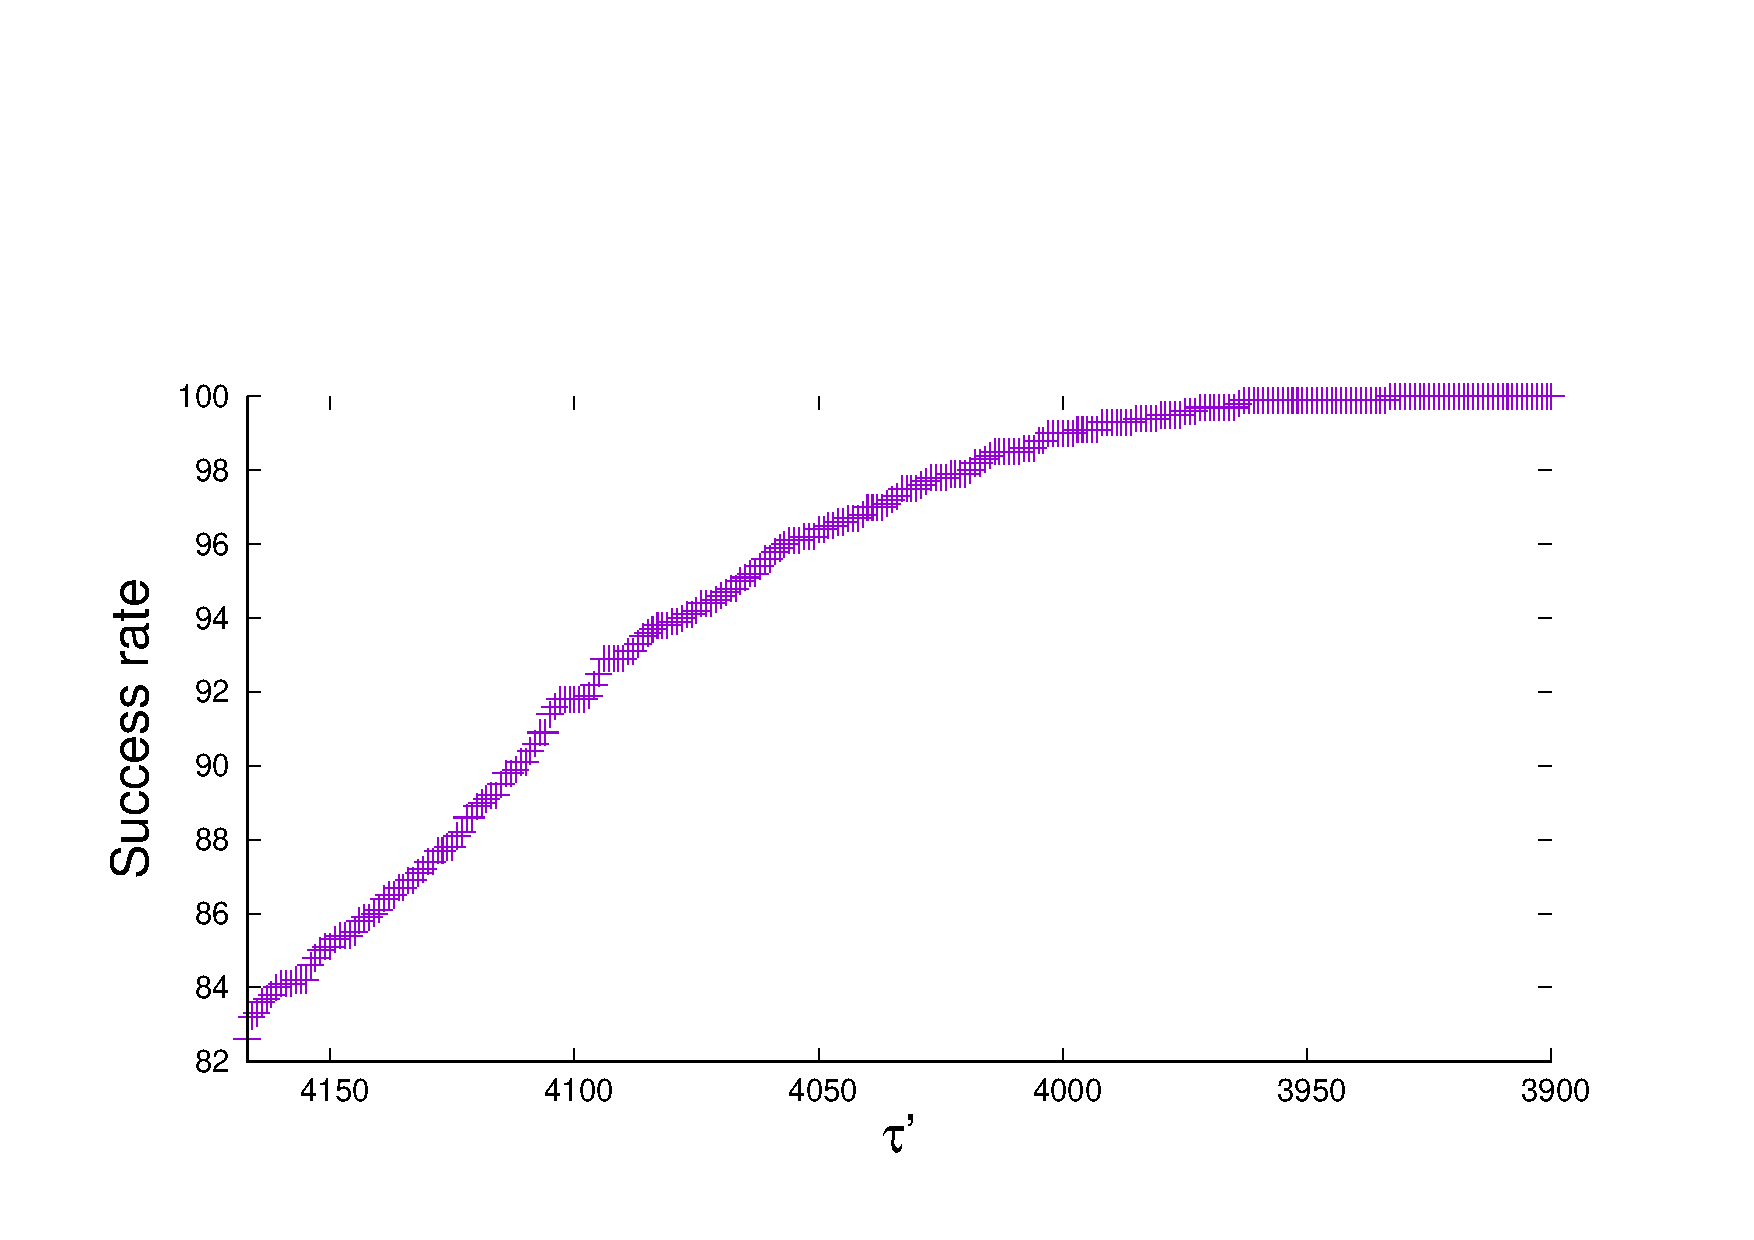
\includegraphics[width = 0.8\textwidth]{distribtau.pdf}
       %% GNUPLOT: LaTeX picture
\setlength{\unitlength}{0.240900pt}
\ifx\plotpoint\undefined\newsavebox{\plotpoint}\fi
\sbox{\plotpoint}{\rule[-0.200pt]{0.400pt}{0.400pt}}%
\begin{picture}(1500,900)(0,0)
\sbox{\plotpoint}{\rule[-0.200pt]{0.400pt}{0.400pt}}%
\put(171.0,131.0){\rule[-0.200pt]{4.818pt}{0.400pt}}
\put(151,131){\makebox(0,0)[r]{$0$}}
\put(1279.0,131.0){\rule[-0.200pt]{4.818pt}{0.400pt}}
\put(171.0,212.0){\rule[-0.200pt]{4.818pt}{0.400pt}}
\put(151,212){\makebox(0,0)[r]{$1000$}}
\put(1279.0,212.0){\rule[-0.200pt]{4.818pt}{0.400pt}}
\put(171.0,293.0){\rule[-0.200pt]{4.818pt}{0.400pt}}
\put(151,293){\makebox(0,0)[r]{$2000$}}
\put(1279.0,293.0){\rule[-0.200pt]{4.818pt}{0.400pt}}
\put(171.0,374.0){\rule[-0.200pt]{4.818pt}{0.400pt}}
\put(151,374){\makebox(0,0)[r]{$3000$}}
\put(1279.0,374.0){\rule[-0.200pt]{4.818pt}{0.400pt}}
\put(171.0,455.0){\rule[-0.200pt]{4.818pt}{0.400pt}}
\put(151,455){\makebox(0,0)[r]{$4000$}}
\put(1279.0,455.0){\rule[-0.200pt]{4.818pt}{0.400pt}}
\put(171.0,535.0){\rule[-0.200pt]{4.818pt}{0.400pt}}
\put(151,535){\makebox(0,0)[r]{$5000$}}
\put(1279.0,535.0){\rule[-0.200pt]{4.818pt}{0.400pt}}
\put(171.0,616.0){\rule[-0.200pt]{4.818pt}{0.400pt}}
\put(151,616){\makebox(0,0)[r]{$6000$}}
\put(1279.0,616.0){\rule[-0.200pt]{4.818pt}{0.400pt}}
\put(171.0,697.0){\rule[-0.200pt]{4.818pt}{0.400pt}}
\put(151,697){\makebox(0,0)[r]{$7000$}}
\put(1279.0,697.0){\rule[-0.200pt]{4.818pt}{0.400pt}}
\put(171.0,778.0){\rule[-0.200pt]{4.818pt}{0.400pt}}
\put(151,778){\makebox(0,0)[r]{$8000$}}
\put(1279.0,778.0){\rule[-0.200pt]{4.818pt}{0.400pt}}
\put(171.0,859.0){\rule[-0.200pt]{4.818pt}{0.400pt}}
\put(151,859){\makebox(0,0)[r]{$9000$}}
\put(1279.0,859.0){\rule[-0.200pt]{4.818pt}{0.400pt}}
\put(171.0,131.0){\rule[-0.200pt]{0.400pt}{4.818pt}}
\put(171,90){\makebox(0,0){$20000$}}
\put(171.0,839.0){\rule[-0.200pt]{0.400pt}{4.818pt}}
\put(359.0,131.0){\rule[-0.200pt]{0.400pt}{4.818pt}}
\put(359,90){\makebox(0,0){$25000$}}
\put(359.0,839.0){\rule[-0.200pt]{0.400pt}{4.818pt}}
\put(547.0,131.0){\rule[-0.200pt]{0.400pt}{4.818pt}}
\put(547,90){\makebox(0,0){$30000$}}
\put(547.0,839.0){\rule[-0.200pt]{0.400pt}{4.818pt}}
\put(735.0,131.0){\rule[-0.200pt]{0.400pt}{4.818pt}}
\put(735,90){\makebox(0,0){$35000$}}
\put(735.0,839.0){\rule[-0.200pt]{0.400pt}{4.818pt}}
\put(923.0,131.0){\rule[-0.200pt]{0.400pt}{4.818pt}}
\put(923,90){\makebox(0,0){$40000$}}
\put(923.0,839.0){\rule[-0.200pt]{0.400pt}{4.818pt}}
\put(1111.0,131.0){\rule[-0.200pt]{0.400pt}{4.818pt}}
\put(1111,90){\makebox(0,0){$45000$}}
\put(1111.0,839.0){\rule[-0.200pt]{0.400pt}{4.818pt}}
\put(1299.0,131.0){\rule[-0.200pt]{0.400pt}{4.818pt}}
\put(1299,90){\makebox(0,0){$50000$}}
\put(1299.0,839.0){\rule[-0.200pt]{0.400pt}{4.818pt}}
\put(171.0,131.0){\rule[-0.200pt]{0.400pt}{175.375pt}}
\put(171.0,131.0){\rule[-0.200pt]{271.735pt}{0.400pt}}
\put(30,495){\makebox(0,0){Needed Flexibility}}
\put(735,29){\makebox(0,0){Period}}
\put(171.0,455.0){\rule[-0.200pt]{0.400pt}{81.183pt}}
\put(171.0,455.0){\rule[-0.200pt]{2.409pt}{0.400pt}}
\put(171.0,792.0){\rule[-0.200pt]{2.409pt}{0.400pt}}
\put(209.0,412.0){\rule[-0.200pt]{0.400pt}{73.715pt}}
\put(199.0,412.0){\rule[-0.200pt]{4.818pt}{0.400pt}}
\put(199.0,718.0){\rule[-0.200pt]{4.818pt}{0.400pt}}
\put(246.0,353.0){\rule[-0.200pt]{0.400pt}{79.497pt}}
\put(236.0,353.0){\rule[-0.200pt]{4.818pt}{0.400pt}}
\put(236.0,683.0){\rule[-0.200pt]{4.818pt}{0.400pt}}
\put(284.0,336.0){\rule[-0.200pt]{0.400pt}{75.883pt}}
\put(274.0,336.0){\rule[-0.200pt]{4.818pt}{0.400pt}}
\put(274.0,651.0){\rule[-0.200pt]{4.818pt}{0.400pt}}
\put(321.0,306.0){\rule[-0.200pt]{0.400pt}{70.343pt}}
\put(311.0,306.0){\rule[-0.200pt]{4.818pt}{0.400pt}}
\put(311.0,598.0){\rule[-0.200pt]{4.818pt}{0.400pt}}
\put(359.0,297.0){\rule[-0.200pt]{0.400pt}{73.715pt}}
\put(349.0,297.0){\rule[-0.200pt]{4.818pt}{0.400pt}}
\put(349.0,603.0){\rule[-0.200pt]{4.818pt}{0.400pt}}
\put(397.0,270.0){\rule[-0.200pt]{0.400pt}{63.598pt}}
\put(387.0,270.0){\rule[-0.200pt]{4.818pt}{0.400pt}}
\put(387.0,534.0){\rule[-0.200pt]{4.818pt}{0.400pt}}
\put(434.0,269.0){\rule[-0.200pt]{0.400pt}{64.561pt}}
\put(424.0,269.0){\rule[-0.200pt]{4.818pt}{0.400pt}}
\put(424.0,537.0){\rule[-0.200pt]{4.818pt}{0.400pt}}
\put(472.0,238.0){\rule[-0.200pt]{0.400pt}{69.138pt}}
\put(462.0,238.0){\rule[-0.200pt]{4.818pt}{0.400pt}}
\put(462.0,525.0){\rule[-0.200pt]{4.818pt}{0.400pt}}
\put(509.0,226.0){\rule[-0.200pt]{0.400pt}{62.393pt}}
\put(499.0,226.0){\rule[-0.200pt]{4.818pt}{0.400pt}}
\put(499.0,485.0){\rule[-0.200pt]{4.818pt}{0.400pt}}
\put(547.0,222.0){\rule[-0.200pt]{0.400pt}{60.225pt}}
\put(537.0,222.0){\rule[-0.200pt]{4.818pt}{0.400pt}}
\put(537.0,472.0){\rule[-0.200pt]{4.818pt}{0.400pt}}
\put(585.0,195.0){\rule[-0.200pt]{0.400pt}{60.225pt}}
\put(575.0,195.0){\rule[-0.200pt]{4.818pt}{0.400pt}}
\put(575.0,445.0){\rule[-0.200pt]{4.818pt}{0.400pt}}
\put(622.0,185.0){\rule[-0.200pt]{0.400pt}{58.780pt}}
\put(612.0,185.0){\rule[-0.200pt]{4.818pt}{0.400pt}}
\put(612.0,429.0){\rule[-0.200pt]{4.818pt}{0.400pt}}
\put(660.0,178.0){\rule[-0.200pt]{0.400pt}{59.743pt}}
\put(650.0,178.0){\rule[-0.200pt]{4.818pt}{0.400pt}}
\put(650.0,426.0){\rule[-0.200pt]{4.818pt}{0.400pt}}
\put(697.0,188.0){\rule[-0.200pt]{0.400pt}{59.020pt}}
\put(687.0,188.0){\rule[-0.200pt]{4.818pt}{0.400pt}}
\put(687.0,433.0){\rule[-0.200pt]{4.818pt}{0.400pt}}
\put(735.0,152.0){\rule[-0.200pt]{0.400pt}{55.889pt}}
\put(725.0,152.0){\rule[-0.200pt]{4.818pt}{0.400pt}}
\put(725.0,384.0){\rule[-0.200pt]{4.818pt}{0.400pt}}
\put(773.0,146.0){\rule[-0.200pt]{0.400pt}{57.575pt}}
\put(763.0,146.0){\rule[-0.200pt]{4.818pt}{0.400pt}}
\put(763.0,385.0){\rule[-0.200pt]{4.818pt}{0.400pt}}
\put(810.0,146.0){\rule[-0.200pt]{0.400pt}{54.925pt}}
\put(800.0,146.0){\rule[-0.200pt]{4.818pt}{0.400pt}}
\put(800.0,374.0){\rule[-0.200pt]{4.818pt}{0.400pt}}
\put(848.0,143.0){\rule[-0.200pt]{0.400pt}{56.371pt}}
\put(838.0,143.0){\rule[-0.200pt]{4.818pt}{0.400pt}}
\put(838.0,377.0){\rule[-0.200pt]{4.818pt}{0.400pt}}
\put(885.0,140.0){\rule[-0.200pt]{0.400pt}{56.371pt}}
\put(875.0,140.0){\rule[-0.200pt]{4.818pt}{0.400pt}}
\put(875.0,374.0){\rule[-0.200pt]{4.818pt}{0.400pt}}
\put(923.0,133.0){\rule[-0.200pt]{0.400pt}{54.202pt}}
\put(913.0,133.0){\rule[-0.200pt]{4.818pt}{0.400pt}}
\put(913.0,358.0){\rule[-0.200pt]{4.818pt}{0.400pt}}
\put(961.0,131.0){\rule[-0.200pt]{0.400pt}{55.166pt}}
\put(951.0,131.0){\rule[-0.200pt]{4.818pt}{0.400pt}}
\put(951.0,360.0){\rule[-0.200pt]{4.818pt}{0.400pt}}
\put(998.0,131.0){\rule[-0.200pt]{0.400pt}{49.384pt}}
\put(988.0,131.0){\rule[-0.200pt]{4.818pt}{0.400pt}}
\put(988.0,336.0){\rule[-0.200pt]{4.818pt}{0.400pt}}
\put(1036.0,131.0){\rule[-0.200pt]{0.400pt}{48.180pt}}
\put(1026.0,131.0){\rule[-0.200pt]{4.818pt}{0.400pt}}
\put(1026.0,331.0){\rule[-0.200pt]{4.818pt}{0.400pt}}
\put(1073.0,131.0){\rule[-0.200pt]{0.400pt}{47.216pt}}
\put(1063.0,131.0){\rule[-0.200pt]{4.818pt}{0.400pt}}
\put(1063.0,327.0){\rule[-0.200pt]{4.818pt}{0.400pt}}
\put(1111.0,131.0){\rule[-0.200pt]{0.400pt}{46.975pt}}
\put(1101.0,131.0){\rule[-0.200pt]{4.818pt}{0.400pt}}
\put(1101.0,326.0){\rule[-0.200pt]{4.818pt}{0.400pt}}
\put(1149.0,131.0){\rule[-0.200pt]{0.400pt}{45.048pt}}
\put(1139.0,131.0){\rule[-0.200pt]{4.818pt}{0.400pt}}
\put(1139.0,318.0){\rule[-0.200pt]{4.818pt}{0.400pt}}
\put(1186.0,131.0){\rule[-0.200pt]{0.400pt}{46.494pt}}
\put(1176.0,131.0){\rule[-0.200pt]{4.818pt}{0.400pt}}
\put(1176.0,324.0){\rule[-0.200pt]{4.818pt}{0.400pt}}
\put(1224.0,131.0){\rule[-0.200pt]{0.400pt}{45.048pt}}
\put(1214.0,131.0){\rule[-0.200pt]{4.818pt}{0.400pt}}
\put(1214.0,318.0){\rule[-0.200pt]{4.818pt}{0.400pt}}
\put(1261.0,131.0){\rule[-0.200pt]{0.400pt}{41.194pt}}
\put(1251.0,131.0){\rule[-0.200pt]{4.818pt}{0.400pt}}
\put(171,608){\makebox(0,0){$+$}}
\put(209,562){\makebox(0,0){$+$}}
\put(246,503){\makebox(0,0){$+$}}
\put(284,479){\makebox(0,0){$+$}}
\put(321,431){\makebox(0,0){$+$}}
\put(359,429){\makebox(0,0){$+$}}
\put(397,390){\makebox(0,0){$+$}}
\put(434,382){\makebox(0,0){$+$}}
\put(472,367){\makebox(0,0){$+$}}
\put(509,340){\makebox(0,0){$+$}}
\put(547,327){\makebox(0,0){$+$}}
\put(585,317){\makebox(0,0){$+$}}
\put(622,307){\makebox(0,0){$+$}}
\put(660,302){\makebox(0,0){$+$}}
\put(697,300){\makebox(0,0){$+$}}
\put(735,278){\makebox(0,0){$+$}}
\put(773,273){\makebox(0,0){$+$}}
\put(810,268){\makebox(0,0){$+$}}
\put(848,267){\makebox(0,0){$+$}}
\put(885,254){\makebox(0,0){$+$}}
\put(923,248){\makebox(0,0){$+$}}
\put(961,259){\makebox(0,0){$+$}}
\put(998,234){\makebox(0,0){$+$}}
\put(1036,234){\makebox(0,0){$+$}}
\put(1073,232){\makebox(0,0){$+$}}
\put(1111,228){\makebox(0,0){$+$}}
\put(1149,216){\makebox(0,0){$+$}}
\put(1186,212){\makebox(0,0){$+$}}
\put(1224,227){\makebox(0,0){$+$}}
\put(1261,203){\makebox(0,0){$+$}}
\put(1251.0,302.0){\rule[-0.200pt]{4.818pt}{0.400pt}}
\put(171.0,131.0){\rule[-0.200pt]{0.400pt}{175.375pt}}
\put(171.0,131.0){\rule[-0.200pt]{271.735pt}{0.400pt}}
\end{picture}

      \end{center}
      \caption{Probability of finding a $(P,\tau')$-assignment over $10,000$ instances}
      \label{fig:spacetau}   
     \end{figure}   

	For more than $80\%$ of the instances, there is an assignment for the maximal size of a datagram $\tau' = \frac{P}{n} = 4166$. This means that \SPMLS perfectly balances the free tics in the period. In the worst case, a solution with $\tau' = 3925$ is found, which still yields at least $3925 - 2500 = 1425$ unused tics between datagrams. Hence, we expect \SPMLS to work well in conjunction with random traffic. 	The excellent performance of \PMLS when the load is high explains this result and further justifies the work we have done to solve \pall efficiently under high load rather than just requiring mild load in applications. 


    \subsubsection{Performance Evaluation}
    
    We evaluate in this section different ways to manage statistical and deterministic traffics together in the same network.
 
    \paragraph{Best-effort datagrams generation}
   Let us denote best-effort by BE. The BE traffic is generated as follows. The size of a BE datagram is small in practice, and set to $50$ tics in our experiments. We generate a random BE traffic in our experiment, such that on average it adds $0.2$ to the load load to obtain a total load of $0.8$. The BE datagrams do not make a round trip in the network as the C-RAN datagrams, they go through a single contention point. 
    We simulate that, by generating independently BE datagrams for each of the two contention points $c_1$ and $c_2$. The \textbf{latency} of a BE datagram is defined as the time it must wait before going through its contention points.

    On each contention point, the generation is split into two exponential distributions which give the time before the next arrival of datagrams~\cite{el2018performance}. The first one models background traffic, corresponding to an average load of $0.15$,  it generates one BE datagram every $333$ tics on average. The second models a burst of BE datagrams, it corresponds to an average load of $0.05$, it generates \emph{ten} BE datagrams at the same time every $10,000$ tics on average. 
    
   	\paragraph{Statistical multiplexing policy}

    We test several policies to deal with all traffics using statistical multiplexing.
   	The BE traffic is managed using \FIFO, and we propose two policies to deal with C-RAN. First, all datagrams, BE or C-RAN, are stored in the same buffer and dealt with the \FIFO policy regardless of their type. We call this policy \FIFO.

    To minimize the latency of C-RAN traffic, we can store the two types of datagrams in two different buffers, managed each with \FIFO, but we prioritize the C-RAN datagrams which are always sent first. It can be technically implemented using TSN 802.1Qbu~\cite{ieee802}, which allows defining priority class in the traffic to schedule first the traffic with the highest priority, here the C-RAN traffic. We call this policy \framepre.
   
   We also consider C-RAN traffic scheduled by \PMLS or \SPMLS. In that case, we need to forbid the transit of a BE datagram that collides with a C-RAN datagram. Thus, in each contention point, we reserve $50$ tics (the size of a BE datagram) before the arrival of a C-RAN message. Observe that it wastes some resources and thus slightly decreases the maximal throughput and may worsen the latency of BE datagrams.
    
    Figure~\ref{fig:belatency} shows the cumulative distribution of the logical latency of BE datagrams, that is the probability that a BE datagram has a latency less than some value.
    The distribution is computed over $1000$ random instances, and for each instance, the traffic is simulated for ten periods.

     \begin{figure}
       \begin{center}
      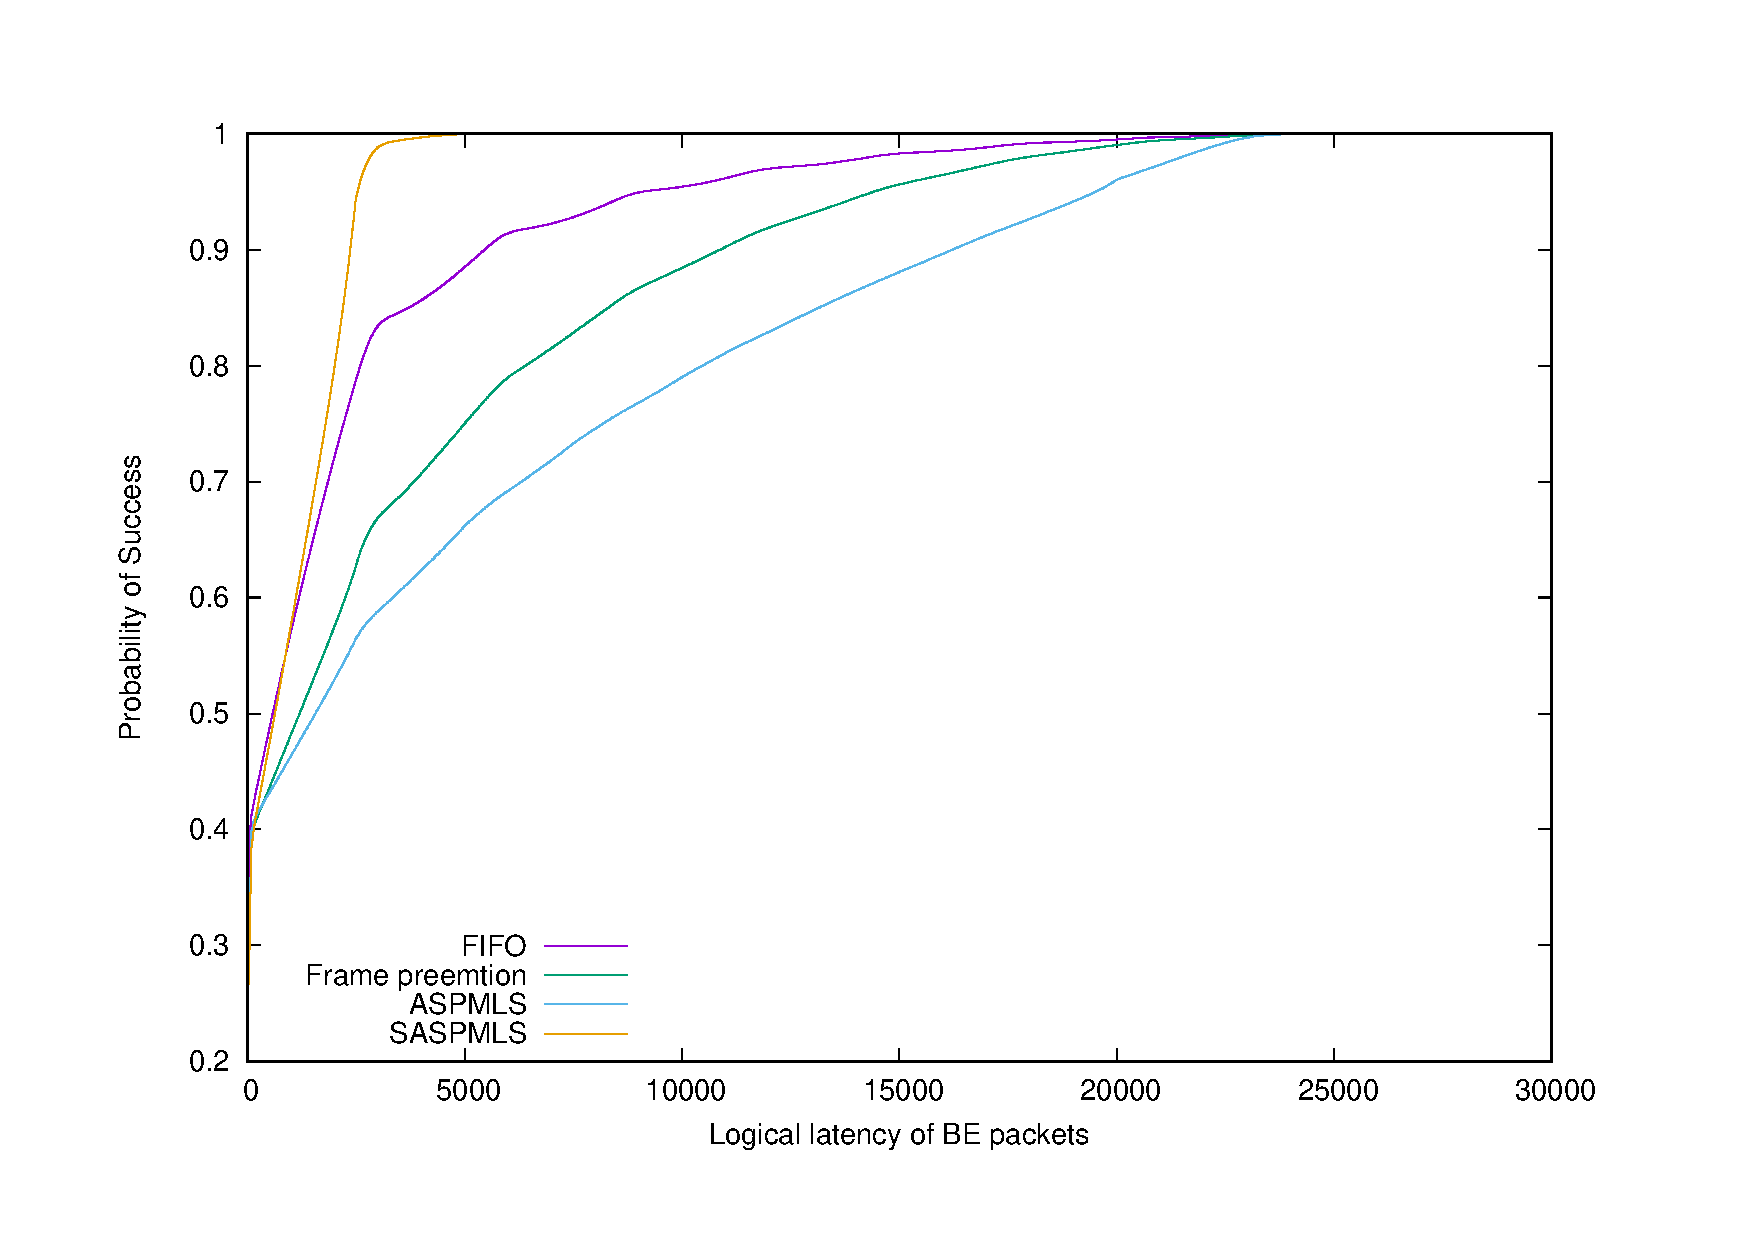
\includegraphics[width = 1\textwidth]{res.pdf}
       %% GNUPLOT: LaTeX picture
\setlength{\unitlength}{0.240900pt}
\ifx\plotpoint\undefined\newsavebox{\plotpoint}\fi
\sbox{\plotpoint}{\rule[-0.200pt]{0.400pt}{0.400pt}}%
\begin{picture}(1500,900)(0,0)
\sbox{\plotpoint}{\rule[-0.200pt]{0.400pt}{0.400pt}}%
\put(171.0,131.0){\rule[-0.200pt]{4.818pt}{0.400pt}}
\put(151,131){\makebox(0,0)[r]{$0$}}
\put(1279.0,131.0){\rule[-0.200pt]{4.818pt}{0.400pt}}
\put(171.0,212.0){\rule[-0.200pt]{4.818pt}{0.400pt}}
\put(151,212){\makebox(0,0)[r]{$1000$}}
\put(1279.0,212.0){\rule[-0.200pt]{4.818pt}{0.400pt}}
\put(171.0,293.0){\rule[-0.200pt]{4.818pt}{0.400pt}}
\put(151,293){\makebox(0,0)[r]{$2000$}}
\put(1279.0,293.0){\rule[-0.200pt]{4.818pt}{0.400pt}}
\put(171.0,374.0){\rule[-0.200pt]{4.818pt}{0.400pt}}
\put(151,374){\makebox(0,0)[r]{$3000$}}
\put(1279.0,374.0){\rule[-0.200pt]{4.818pt}{0.400pt}}
\put(171.0,455.0){\rule[-0.200pt]{4.818pt}{0.400pt}}
\put(151,455){\makebox(0,0)[r]{$4000$}}
\put(1279.0,455.0){\rule[-0.200pt]{4.818pt}{0.400pt}}
\put(171.0,535.0){\rule[-0.200pt]{4.818pt}{0.400pt}}
\put(151,535){\makebox(0,0)[r]{$5000$}}
\put(1279.0,535.0){\rule[-0.200pt]{4.818pt}{0.400pt}}
\put(171.0,616.0){\rule[-0.200pt]{4.818pt}{0.400pt}}
\put(151,616){\makebox(0,0)[r]{$6000$}}
\put(1279.0,616.0){\rule[-0.200pt]{4.818pt}{0.400pt}}
\put(171.0,697.0){\rule[-0.200pt]{4.818pt}{0.400pt}}
\put(151,697){\makebox(0,0)[r]{$7000$}}
\put(1279.0,697.0){\rule[-0.200pt]{4.818pt}{0.400pt}}
\put(171.0,778.0){\rule[-0.200pt]{4.818pt}{0.400pt}}
\put(151,778){\makebox(0,0)[r]{$8000$}}
\put(1279.0,778.0){\rule[-0.200pt]{4.818pt}{0.400pt}}
\put(171.0,859.0){\rule[-0.200pt]{4.818pt}{0.400pt}}
\put(151,859){\makebox(0,0)[r]{$9000$}}
\put(1279.0,859.0){\rule[-0.200pt]{4.818pt}{0.400pt}}
\put(171.0,131.0){\rule[-0.200pt]{0.400pt}{4.818pt}}
\put(171,90){\makebox(0,0){$20000$}}
\put(171.0,839.0){\rule[-0.200pt]{0.400pt}{4.818pt}}
\put(359.0,131.0){\rule[-0.200pt]{0.400pt}{4.818pt}}
\put(359,90){\makebox(0,0){$25000$}}
\put(359.0,839.0){\rule[-0.200pt]{0.400pt}{4.818pt}}
\put(547.0,131.0){\rule[-0.200pt]{0.400pt}{4.818pt}}
\put(547,90){\makebox(0,0){$30000$}}
\put(547.0,839.0){\rule[-0.200pt]{0.400pt}{4.818pt}}
\put(735.0,131.0){\rule[-0.200pt]{0.400pt}{4.818pt}}
\put(735,90){\makebox(0,0){$35000$}}
\put(735.0,839.0){\rule[-0.200pt]{0.400pt}{4.818pt}}
\put(923.0,131.0){\rule[-0.200pt]{0.400pt}{4.818pt}}
\put(923,90){\makebox(0,0){$40000$}}
\put(923.0,839.0){\rule[-0.200pt]{0.400pt}{4.818pt}}
\put(1111.0,131.0){\rule[-0.200pt]{0.400pt}{4.818pt}}
\put(1111,90){\makebox(0,0){$45000$}}
\put(1111.0,839.0){\rule[-0.200pt]{0.400pt}{4.818pt}}
\put(1299.0,131.0){\rule[-0.200pt]{0.400pt}{4.818pt}}
\put(1299,90){\makebox(0,0){$50000$}}
\put(1299.0,839.0){\rule[-0.200pt]{0.400pt}{4.818pt}}
\put(171.0,131.0){\rule[-0.200pt]{0.400pt}{175.375pt}}
\put(171.0,131.0){\rule[-0.200pt]{271.735pt}{0.400pt}}
\put(30,495){\makebox(0,0){Needed Flexibility}}
\put(735,29){\makebox(0,0){Period}}
\put(171.0,455.0){\rule[-0.200pt]{0.400pt}{81.183pt}}
\put(171.0,455.0){\rule[-0.200pt]{2.409pt}{0.400pt}}
\put(171.0,792.0){\rule[-0.200pt]{2.409pt}{0.400pt}}
\put(209.0,412.0){\rule[-0.200pt]{0.400pt}{73.715pt}}
\put(199.0,412.0){\rule[-0.200pt]{4.818pt}{0.400pt}}
\put(199.0,718.0){\rule[-0.200pt]{4.818pt}{0.400pt}}
\put(246.0,353.0){\rule[-0.200pt]{0.400pt}{79.497pt}}
\put(236.0,353.0){\rule[-0.200pt]{4.818pt}{0.400pt}}
\put(236.0,683.0){\rule[-0.200pt]{4.818pt}{0.400pt}}
\put(284.0,336.0){\rule[-0.200pt]{0.400pt}{75.883pt}}
\put(274.0,336.0){\rule[-0.200pt]{4.818pt}{0.400pt}}
\put(274.0,651.0){\rule[-0.200pt]{4.818pt}{0.400pt}}
\put(321.0,306.0){\rule[-0.200pt]{0.400pt}{70.343pt}}
\put(311.0,306.0){\rule[-0.200pt]{4.818pt}{0.400pt}}
\put(311.0,598.0){\rule[-0.200pt]{4.818pt}{0.400pt}}
\put(359.0,297.0){\rule[-0.200pt]{0.400pt}{73.715pt}}
\put(349.0,297.0){\rule[-0.200pt]{4.818pt}{0.400pt}}
\put(349.0,603.0){\rule[-0.200pt]{4.818pt}{0.400pt}}
\put(397.0,270.0){\rule[-0.200pt]{0.400pt}{63.598pt}}
\put(387.0,270.0){\rule[-0.200pt]{4.818pt}{0.400pt}}
\put(387.0,534.0){\rule[-0.200pt]{4.818pt}{0.400pt}}
\put(434.0,269.0){\rule[-0.200pt]{0.400pt}{64.561pt}}
\put(424.0,269.0){\rule[-0.200pt]{4.818pt}{0.400pt}}
\put(424.0,537.0){\rule[-0.200pt]{4.818pt}{0.400pt}}
\put(472.0,238.0){\rule[-0.200pt]{0.400pt}{69.138pt}}
\put(462.0,238.0){\rule[-0.200pt]{4.818pt}{0.400pt}}
\put(462.0,525.0){\rule[-0.200pt]{4.818pt}{0.400pt}}
\put(509.0,226.0){\rule[-0.200pt]{0.400pt}{62.393pt}}
\put(499.0,226.0){\rule[-0.200pt]{4.818pt}{0.400pt}}
\put(499.0,485.0){\rule[-0.200pt]{4.818pt}{0.400pt}}
\put(547.0,222.0){\rule[-0.200pt]{0.400pt}{60.225pt}}
\put(537.0,222.0){\rule[-0.200pt]{4.818pt}{0.400pt}}
\put(537.0,472.0){\rule[-0.200pt]{4.818pt}{0.400pt}}
\put(585.0,195.0){\rule[-0.200pt]{0.400pt}{60.225pt}}
\put(575.0,195.0){\rule[-0.200pt]{4.818pt}{0.400pt}}
\put(575.0,445.0){\rule[-0.200pt]{4.818pt}{0.400pt}}
\put(622.0,185.0){\rule[-0.200pt]{0.400pt}{58.780pt}}
\put(612.0,185.0){\rule[-0.200pt]{4.818pt}{0.400pt}}
\put(612.0,429.0){\rule[-0.200pt]{4.818pt}{0.400pt}}
\put(660.0,178.0){\rule[-0.200pt]{0.400pt}{59.743pt}}
\put(650.0,178.0){\rule[-0.200pt]{4.818pt}{0.400pt}}
\put(650.0,426.0){\rule[-0.200pt]{4.818pt}{0.400pt}}
\put(697.0,188.0){\rule[-0.200pt]{0.400pt}{59.020pt}}
\put(687.0,188.0){\rule[-0.200pt]{4.818pt}{0.400pt}}
\put(687.0,433.0){\rule[-0.200pt]{4.818pt}{0.400pt}}
\put(735.0,152.0){\rule[-0.200pt]{0.400pt}{55.889pt}}
\put(725.0,152.0){\rule[-0.200pt]{4.818pt}{0.400pt}}
\put(725.0,384.0){\rule[-0.200pt]{4.818pt}{0.400pt}}
\put(773.0,146.0){\rule[-0.200pt]{0.400pt}{57.575pt}}
\put(763.0,146.0){\rule[-0.200pt]{4.818pt}{0.400pt}}
\put(763.0,385.0){\rule[-0.200pt]{4.818pt}{0.400pt}}
\put(810.0,146.0){\rule[-0.200pt]{0.400pt}{54.925pt}}
\put(800.0,146.0){\rule[-0.200pt]{4.818pt}{0.400pt}}
\put(800.0,374.0){\rule[-0.200pt]{4.818pt}{0.400pt}}
\put(848.0,143.0){\rule[-0.200pt]{0.400pt}{56.371pt}}
\put(838.0,143.0){\rule[-0.200pt]{4.818pt}{0.400pt}}
\put(838.0,377.0){\rule[-0.200pt]{4.818pt}{0.400pt}}
\put(885.0,140.0){\rule[-0.200pt]{0.400pt}{56.371pt}}
\put(875.0,140.0){\rule[-0.200pt]{4.818pt}{0.400pt}}
\put(875.0,374.0){\rule[-0.200pt]{4.818pt}{0.400pt}}
\put(923.0,133.0){\rule[-0.200pt]{0.400pt}{54.202pt}}
\put(913.0,133.0){\rule[-0.200pt]{4.818pt}{0.400pt}}
\put(913.0,358.0){\rule[-0.200pt]{4.818pt}{0.400pt}}
\put(961.0,131.0){\rule[-0.200pt]{0.400pt}{55.166pt}}
\put(951.0,131.0){\rule[-0.200pt]{4.818pt}{0.400pt}}
\put(951.0,360.0){\rule[-0.200pt]{4.818pt}{0.400pt}}
\put(998.0,131.0){\rule[-0.200pt]{0.400pt}{49.384pt}}
\put(988.0,131.0){\rule[-0.200pt]{4.818pt}{0.400pt}}
\put(988.0,336.0){\rule[-0.200pt]{4.818pt}{0.400pt}}
\put(1036.0,131.0){\rule[-0.200pt]{0.400pt}{48.180pt}}
\put(1026.0,131.0){\rule[-0.200pt]{4.818pt}{0.400pt}}
\put(1026.0,331.0){\rule[-0.200pt]{4.818pt}{0.400pt}}
\put(1073.0,131.0){\rule[-0.200pt]{0.400pt}{47.216pt}}
\put(1063.0,131.0){\rule[-0.200pt]{4.818pt}{0.400pt}}
\put(1063.0,327.0){\rule[-0.200pt]{4.818pt}{0.400pt}}
\put(1111.0,131.0){\rule[-0.200pt]{0.400pt}{46.975pt}}
\put(1101.0,131.0){\rule[-0.200pt]{4.818pt}{0.400pt}}
\put(1101.0,326.0){\rule[-0.200pt]{4.818pt}{0.400pt}}
\put(1149.0,131.0){\rule[-0.200pt]{0.400pt}{45.048pt}}
\put(1139.0,131.0){\rule[-0.200pt]{4.818pt}{0.400pt}}
\put(1139.0,318.0){\rule[-0.200pt]{4.818pt}{0.400pt}}
\put(1186.0,131.0){\rule[-0.200pt]{0.400pt}{46.494pt}}
\put(1176.0,131.0){\rule[-0.200pt]{4.818pt}{0.400pt}}
\put(1176.0,324.0){\rule[-0.200pt]{4.818pt}{0.400pt}}
\put(1224.0,131.0){\rule[-0.200pt]{0.400pt}{45.048pt}}
\put(1214.0,131.0){\rule[-0.200pt]{4.818pt}{0.400pt}}
\put(1214.0,318.0){\rule[-0.200pt]{4.818pt}{0.400pt}}
\put(1261.0,131.0){\rule[-0.200pt]{0.400pt}{41.194pt}}
\put(1251.0,131.0){\rule[-0.200pt]{4.818pt}{0.400pt}}
\put(171,608){\makebox(0,0){$+$}}
\put(209,562){\makebox(0,0){$+$}}
\put(246,503){\makebox(0,0){$+$}}
\put(284,479){\makebox(0,0){$+$}}
\put(321,431){\makebox(0,0){$+$}}
\put(359,429){\makebox(0,0){$+$}}
\put(397,390){\makebox(0,0){$+$}}
\put(434,382){\makebox(0,0){$+$}}
\put(472,367){\makebox(0,0){$+$}}
\put(509,340){\makebox(0,0){$+$}}
\put(547,327){\makebox(0,0){$+$}}
\put(585,317){\makebox(0,0){$+$}}
\put(622,307){\makebox(0,0){$+$}}
\put(660,302){\makebox(0,0){$+$}}
\put(697,300){\makebox(0,0){$+$}}
\put(735,278){\makebox(0,0){$+$}}
\put(773,273){\makebox(0,0){$+$}}
\put(810,268){\makebox(0,0){$+$}}
\put(848,267){\makebox(0,0){$+$}}
\put(885,254){\makebox(0,0){$+$}}
\put(923,248){\makebox(0,0){$+$}}
\put(961,259){\makebox(0,0){$+$}}
\put(998,234){\makebox(0,0){$+$}}
\put(1036,234){\makebox(0,0){$+$}}
\put(1073,232){\makebox(0,0){$+$}}
\put(1111,228){\makebox(0,0){$+$}}
\put(1149,216){\makebox(0,0){$+$}}
\put(1186,212){\makebox(0,0){$+$}}
\put(1224,227){\makebox(0,0){$+$}}
\put(1261,203){\makebox(0,0){$+$}}
\put(1251.0,302.0){\rule[-0.200pt]{4.818pt}{0.400pt}}
\put(171.0,131.0){\rule[-0.200pt]{0.400pt}{175.375pt}}
\put(171.0,131.0){\rule[-0.200pt]{271.735pt}{0.400pt}}
\end{picture}

      \end{center}
      \caption{Cumulative distribution of the latency of BE datagrams for several network management schemes}
      \label{fig:belatency}   
     \end{figure}    
     

     If we compare \FIFO and \framepre, we see that the latency of BE datagrams is better ($1977$ tics on average) with \FIFO. It is expected since in \framepre the C-RAN datagrams are prioritized and thus 
     the latency of the BE datagrams is strictly worse, $3256$ tics on average. However, this is a trade-off with the margin of the C-RAN datagrams, which is strictly better for \framepre: $1919$ tics on average versus $5265$ tics for \FIFO. 

     Using a deterministic approach for C-RAN with \PMLS, the trade-off is even stronger:
      the C-RAN margin is down to $0$, but the BE traffic is more impacted, with a latency of $4909$ tics on average. This can be explained by both reservation of tics to deal with the periodic sending scheme and the long sequences of C-RAN datagrams without free time in contention points.
     
     Using \SPMLS, the C-RAN traffic is smoothed over the period, to regularly leave some free tics for BE traffic. By construction, we still have C-RAN margin of $0$ but it improves the latency of BE datagrams to $949$ tics on average, which is even better than with \FIFO. 
     
      This result shows that managing deterministic traffic deterministically is also good for the stochastic sources of traffic in the network. We have already observed such a phenomenon in~\cite{DBLP:conf/ondm/BarthGS19}, a similar problem on an optical ring.
     


 \section{Conclusion}
 
	In this article, we proposed two kinds of deterministic sending schemes to establish low latency periodic communication between BBUs and RRHs in a fronthaul network. We have shown 
    that finding these schemes is $\NP$-complete even for simple networks of width $2$ or depth $2$. Hence, we focus on solving them on star routed networks, which are even simpler, 
    but model practical fronthaul networks.
    
    The first kind of sending scheme uses no buffering and has no latency overhead. Such schemes exist and can be found when the routes are short (using algorithm \shortestlongest) or when the load is less than $0.8$ and the number of routes is at most $20$ (using algorithm \ESCA).  
	When the load is higher, buffering is allowed in the BBUs and we propose the algorithm \PMLS to find a deterministic communication scheme with almost no additional logical latency.
    We have compared algorithm \PMLS to other alternatives and in particular we show it is on par with \ASPMLS, which uses an FPT optimal subroutine instead of an almost linear time heuristic.

 	Our deterministic approach is vastly superior to the classical statistical multiplexing for all loads of the network, even when sources of random traffic are present. Indeed, even with an oversized network (small load), the latency of statistical multiplexing is an order of magnitude larger than what is required, while our solution requires zero logical latency for most instances even in the harshest settings. This emphasizes that \emph{deterministic sources} of traffic are always best \emph{dealt with deterministically}.  
    
 	There are still several challenges to tackle so that our work can be easily used in a real fronthaul network for C-RAN. 
  	From a theoretical perspective, we need to prove that \pazl and \pall are $\NP$-hard on star routed networks. Then, we should design a better \FPT algorithm for \pall on star routed networks, as efficient as the one for \pazl. This would help us understand if any performance is lost by using \PMLS as a heuristic in practice. Then, we must generalize our study of the \pall problem to other common fronthaul topologies, such as caterpillars, trees, cycles, or bounded treewidth graphs. Some elements on cycle topologies are given in~\cite{DBLP:conf/ondm/BarthGS19} and on routed networks of bounded contention depth, for synchronized RRHs in~\cite{guiraud2020synchronized}.


   	Several variations of our model are relevant to capture more use cases than C-RAN. 
   	We may consider routes periodically emitting datagrams of \emph{different sizes} to represent different payloads transmitted in the network. In that case, we cannot rely on \PMLS since the corresponding scheduling problem is already $\NP$-hard. 
   	We could also allow for links of different speeds in the fronthaul network, but we must then model
   	the interface between links more precisely, which is tedious but could be solved using scheduling over several parallel machines using~\cite{simons1989fast}.
	Instead of minimizing the worst transmission time, we may want to minimize the average transmission time. This objective is linear, and it makes the size of the route irrelevant to the objective. Hence, it should be \emph{easier} to solve, for instance using linear programming. We could allow preemption, that is the datagrams may be cut into pieces, which would certainly change the complexity of the problem and help with the latency.  
   	Instead of computing periodic sending schemes, we could try to organize communications with pseudo-periodic schemes (periodic over several periods). Finally, the routes may not be fixed but computed from the network to minimize $TR(A)$, which makes the problem even more difficult to solve. 





 	\paragraph*{Acknowledgments} 
 	We thank Olivier Marcé and Brice Leclerc who have introduced us to the problem, from a practical perspective. We also thank Christian Cad\'er\'e and David Auger for friendly discussions on the subject and insightful remarks. This work has been partially supported by the french ANR project N-GREEN.

\bibliographystyle{ieeetr}
\bibliography{Sources}

\end{document}
